\documentclass{article}

\usepackage[utf8]{inputenc}
\usepackage{xcolor}
\usepackage{graphicx}
\usepackage{float}
\usepackage[margin=0.8in]{geometry}
\usepackage[italian]{babel}
\usepackage{hyperref}
\usepackage{minted}

\graphicspath{{./images/}}

\title{Relazione Progetto Basi di Dati \\ A.A. 2021 - 2022}
\author{Antonutti Marco (142426),
        \and Candolo Vittorio Giorgio (141879),
        \and Pipan Martin (151699),
        \and Pozzana Matteo (142250)}
\date{Ottobre 2022}
\begin{document}
\maketitle

\newpage
\renewcommand{\contentsname}{Indice}
\tableofcontents

\newpage

\section{Introduzione}
L'elaborato tratta l'attività di progettazione e di implementazione di una base di dati relazionale per il sistema informativo di un'azienda.
\newline
\newline
Vengono analizzate in particolare le fasi di raccolta e analisi dei requisiti, progettazione concettuale, progettazione logica, progettazione fisica, implementazione e analisi dei dati.

\newpage

\section{Analisi dei requisiti}

\subsection{Requisiti forniti}
Si è acquisita la descrizione del sistema e del dominio dalla consegna.
\newline
\newline
\setlength{\fboxsep}{1em}
\fbox{
    \parbox{\textwidth}{
        Vogliamo modellare le seguenti informazioni riguardanti gli impiegati di un’azienda, i dipartimenti a cui afferiscono, le competenze che possiedono e i progetti a cui partecipano.
        \newline
        \newline
        Ogni impiegato ha una matricola, assegnatagli dalla società, che lo identifica univocamente. Di ogni impiegato interessano il nome e il cognome, la data di nascita e la data di assunzione. Se un impiegato è coniugato con un altro impiegato della stessa società, interessano la data del matrimonio e il coniuge. Ogni impiegato ha una qualifica (ad esempio, segretario, impiegato, programmatore, analista, progettista, ecc.). Dei laureati e dei segretari interessano anche altre informazioni. Dei laureati interessa il tipo di laurea e dei segretari le lingue conosciute.
        \newline
        \newline
        La società è organizzata in dipartimenti. Ciascun dipartimento è identificato univocamente dal nome e possiede un recapito telefonico. Dipartimenti distinti hanno un diverso recapito telefonico. Ogni impiegato afferisce ad un unico dipartimento. Ogni dipartimento viene rifornito da vari fornitori e un fornitore può rifornire vari dipartimenti. Di ogni fornitore interessano il nome e l’indirizzo.
        \newline
        \newline
        I progetti sono identificati da un numero e sono caratterizzati da una città e da un budget. Più impiegati possono essere coinvolti in uno stesso progetto. Un impiegato può partecipare a più progetti, ma può essere assegnato ad un unico progetto per città. Di ogni città con almeno un progetto, interessano il numero di residenti e la regione di appartenenza. Un impiegato può avere più competenze, ma usarne solo alcune per un particolare progetto. Un impiegato usa ogni sua competenza in almeno un progetto. Ad ogni competenza è assegnato un codice, che la identifica univocamente e una descrizione.
    }
}

\subsection{Glossario}
Pur essendo le specifiche iniziali sostanzialmente univoche nell'uso dei termini, si è deciso di redigere comunque un glossario al fine di meglio analizzare le entità e le relazioni fra esse.
\begin{table}[h]
\renewcommand{\arraystretch}{1.5}
\centering
\begin{tabular}{|p{0.11\textwidth}|p{0.45\textwidth}|p{0.1\textwidth}|p{0.25\textwidth}|}
\hline
\textbf{Termine} & \textbf{Descrizione} & \textbf{Sinonimi} & \textbf{Relazioni}        
\\ \hline
Impiegato & Persona che svolge la propria attività professionale presso l'azienda &   & Dipartimento, Progetto, Competenza
\\ \hline
Dipartimento & Struttura organizzativa interna all'azienda che svolge un determinato compito per l'azienda &  & Fornitore, Impiegato
\\ \hline
Fornitore & Azienda esterna, rifornisce i dipartimenti &  & Dipartimento
\\ \hline
Progetto & Serie di attività svolte dagli impiegati dell'azienda al fine di raggiungere un determinato obiettivo aziendale &    & Città, Competenza, Impiegato
\\ \hline
Città & Centro abitato dove l'azienda svolge i suoi progetti &   & Progetto
\\ \hline
Competenza & Abilità di un impiegato, viene usata per svolgere determinati compiti aziendali &   & Progetto, Impiegato 
\\ \hline
Laureato & Impiegato in possesso di una o più lauree &  & Impiegato (\textit{Specializzazione})
\\ \hline
Segretario & Impiegato che svolge compiti amministrativi o di segreteria & & Impiegato (\textit{Specializzazione})
\\ \hline
\end{tabular}
\end{table}

\newpage

\subsection{Strutturazione dei requisiti}
Eventuali integrazioni alla descrizione fornita o assunzioni fatte sono indicate in \textit{corsivo}.
\begin{table}[H]
\renewcommand{\arraystretch}{1.4}
\centering
\begin{tabular}{|p{1\textwidth}|}
\hline
\multicolumn{1}{|c|}{\textbf{Impiegato}}
\\ \hline
\begin{itemize}
\item Identificato univocamente da una matricola e caratterizzato da nome, cognome, data di nascita, data di assunzione e qualifica.
\newline
\item Se coniugato con altro impiegato è ulteriormente caratterizzato dalla data di matrimonio col coniuge.
\newline
\item Se segretario è ulteriormente caratterizzato dalle lingue conosciute.
\newline
\item Se laureato è ulteriormente caratterizzato dal tipo di laurea.
\newline
\item Ogni impiegato afferisce ad un unico dipartimento.
\newline
\item Ogni impiegato può partecipare a più progetti ma ad uno solo per città.
\newline
\item Ogni impiegato usa ogni sua competenza in almeno un progetto.
\end{itemize}
\\ \hline
\multicolumn{1}{|c|}{\textbf{Dipartimento}}
\\ \hline
\begin{itemize}
\item Identificato univocamente dal nome e caratterizzato da un recapito telefonico univoco.
\end{itemize}
\\ \hline
\multicolumn{1}{|c|}{\textbf{Fornitore}}
\\ \hline
\begin{itemize}
\item \textit{Identificato univocamente dalla partita IVA} e caratterizzato dal nome e dall'indirizzo.
\newline
\item Ogni fornitore può rifornire diversi dipartimenti.
\end{itemize}
\\ \hline
\multicolumn{1}{|c|}{\textbf{Progetto}}
\\ \hline
\begin{itemize}
\item Identificato univocamente da un numero e caratterizzato dalla città dove si svolge e da un budget.
\end{itemize}
\\ \hline
\multicolumn{1}{|c|}{\textbf{Città}}
\\ \hline
\begin{itemize}
\item \textit{Identificata univocamente dal nome e dalla regione} e caratterizzata da numero di residenti e regione di appartenenza.
\end{itemize}
\\ \hline
\multicolumn{1}{|c|}{\textbf{Competenza}}
\\ \hline
\begin{itemize}
\item Identificata univocamente da un codice e caratterizzata da una descrizione.
\end{itemize}
\\ \hline
\end{tabular}
\end{table}

\newpage

\subsection{Rappresentazione dei concetti}
Ogni {\color{red} impiegato} ha una {\color{magenta}matricola}, assegnatagli dalla società, che lo identifica univocamente.
\newline
Di ogni impiegato interessano il {\color{magenta}nome} e il {\color{magenta}cognome}, la {\color{magenta}data di nascita} e la {\color{magenta}data di assunzione}.
\newline
Se un impiegato è {\color{blue}coniugato} con un altro impiegato della stessa società, interessano la {\color{teal}data del matrimonio} e il coniuge.
\newline
Ogni impiegato ha una {\color{magenta}qualifica} (ad esempio, segretario, impiegato, programmatore, analista, progettista, ecc.).
\newline
Dei {\color{orange}laureati} e dei {\color{orange}segretari} interessano anche altre informazioni.
\newline
Dei laureati interessa il {\color{magenta}tipo di laurea} e dei segretari le {\color{magenta}lingue conosciute}.
\newline
\newline
La società è organizzata in {\color{red} dipartimenti}.
\newline
Ciascun dipartimento è identificato univocamente dal {\color{magenta}nome} e possiede uno {\color{magenta}recapito telefonico}.
\newline
Dipartimenti distinti hanno un diverso recapito telefonico.
\newline
Ogni impiegato {\color{blue}afferisce} ad un unico dipartimento. 
\newline
Ogni dipartimento viene {\color{blue}rifornito} da vari {\color{red} fornitori} e un fornitore può rifornire vari dipartimenti.
\newline
Di ogni fornitore interessano il {\color{magenta}nome} e l’{\color{magenta}indirizzo}.
\newline
\newline
I {\color{red} progetti} sono identificati da un {\color{magenta}numero} e sono caratterizzati da una {\color{blue}città} e da un {\color{magenta}budget}.
\newline
Più impiegati possono essere coinvolti in uno stesso progetto.
\newline
Un impiegato può {\color{blue}partecipare} a più progetti, ma può essere assegnato ad un unico progetto per {\color{red} città}.
\newline
Di ogni città con almeno un progetto, interessano il {\color{magenta}numero} di residenti e la {\color{magenta}regione} di appartenenza.
\newline
Un impiegato può {\color{blue}avere} più {\color{red} competenze}, ma usarne solo alcune per un particolare progetto.
\newline
Un impiegato usa ogni sua competenza in almeno un progetto.
\newline
Ad ogni competenza è assegnato un {\color{magenta}codice}, che la identifica univocamente, e una {\color{magenta}descrizione}.

\subsubsection*{Legenda}
{\color{red}Entità}
\newline
{\color{orange}Specializzazione}
\newline
{\color{magenta}Attributo}
\newline
{\color{blue}Relazione}
\newline
{\color{teal}Attributo di relazione}

\subsection{Integrazioni e riepilogo delle assunzioni fatte}
In conclusione della fase di analisi dei requisiti si è provveduto ad integrare la consegna di due attributi derivati, al fine di poter svolgere le opportune analisi e modellazioni nelle fasi successive del progetto:
\newline
\newline
Dipartimento - numero fornitori.
\newline
Impiegato - numero progetti.
\newline
\newline
Si vogliono inoltre ricapitolare le assunzioni e le scelte fatte per escludere eventuali ambiguità:
\newline
\newline
Le competenze degli impiegati costituiscono un'entità e sono da intendersi come applicazioni delle qualifiche.
\newline
Le qualifiche invece rimangono attributo degli impiegati come richiesto dalla consegna.
\newline
\newline
Laureati e segretari sono specializzazioni dell'entità Impiegato.
\newline
Tipo di laurea e lingue conosciute sono, rispettivamente, attributi della prima e della seconda specializzazione.
\newline

\newpage

\section{Progettazione Concettuale}

\subsection{Diagramma ER}
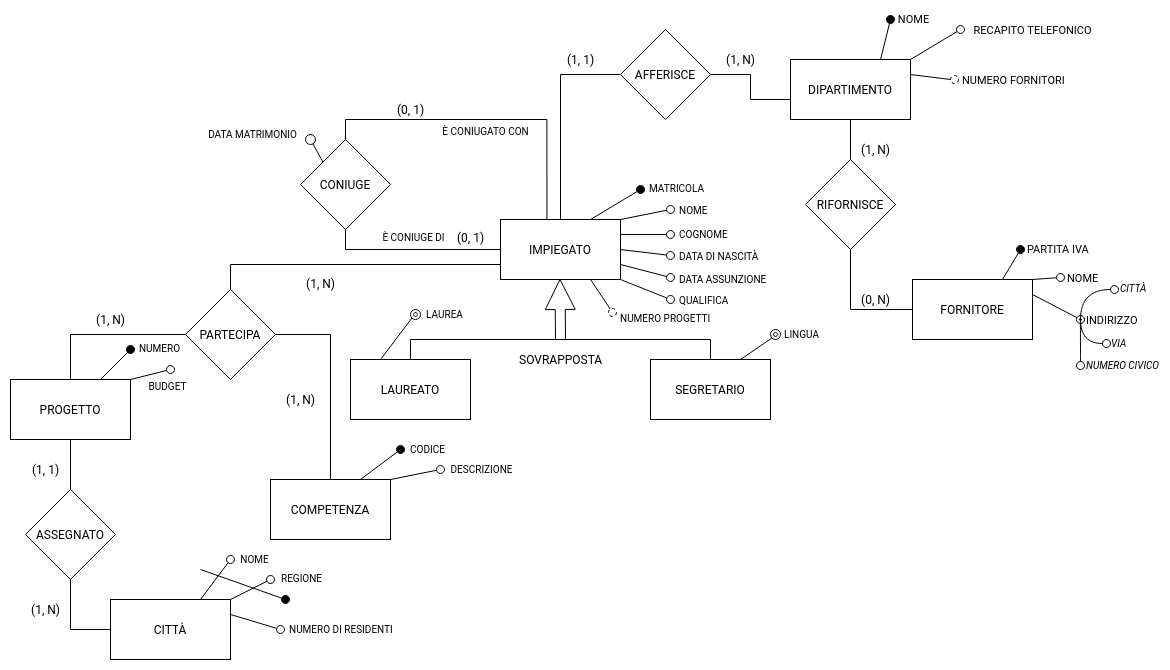
\includegraphics[width=\textwidth]{er.png}

\subsubsection*{Legenda}
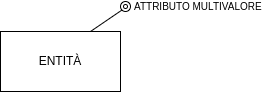
\includegraphics[width=.2\textwidth]{multivalore.png}
\newline
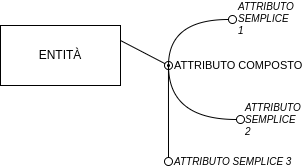
\includegraphics[width=.2\textwidth]{composto.png}

\newpage

\subsection{Vincoli aziendali}
Al fine di codificare i vincoli imposti dai requisiti del progetto si è definito il seguente vincolo aziendale:
\newline
\newline
Un impiegato può partecipare a più progetti, ma non a più di uno per città.

\subsection{Regole di derivazione}
Si esplicitano poi le regole di derivazione per gli attributi derivati introdotti:
\newline
\newline
\textbf{Dipendenti: numero progetti}
\newline
Conta il numero di tuple della relazione partecipa in cui compare un l'impiegato
\newline
\newline
\textbf{Dipartimento: numero fornitori}
\newline
Conta il numero di tuple della relazione rifornisce in cui compare il dipartimento

\newpage

\section{Progettazione Logica}

\subsection{Analisi delle ridondanze}

\subsubsection{Analisi dei cicli}
Lo schema ER non presenta cicli.
\newline
Tuttavia la configurazione scelta prevede il vincolo aziendale descritto in \hyperlink{page.9}{precedenza}.

\subsubsection{Requisiti operazionali}
Partendo da quanto descritto nei requisiti e facendo delle assunzioni al fine di poter svolgere poi delle analisi significative, di seguito vengono formulate le principali operazioni, ciascuna con la rispettiva frequenza.
\begin{table}[H]
\renewcommand{\arraystretch}{1.5}
\centering
\begin{tabular}{|p{0.55\textwidth}|l|l|l|}
\cline{1-3}
Operazione & Tipo & Frequenza\\ \cline{1-3}
Ricerca dei fornitori di un dipartimento & Interattiva & 100/mese \\ \cline{1-3}
Ricerca dei segretari che conoscono una determinata lingua & Interattiva & 15/mese\\ \cline{1-3}
Ricerca degli impiegati con determinata competenza & Interattiva & 200/mese \\ \cline{1-3}
Inserimento di un nuovo progetto & Interattiva & 20/mese \\ \cline{1-3}
Ricerca delle competenze di un impiegato & Interattiva & 200/mese \\ \cline{1-3}
Ricerca di impiegati coniugati & Interattiva & 10/mese \\ \cline{1-3}
Ricerca di impiegati che partecipano ad un progetto nullo & Batch & 4/mese \\ \cline{1-3}
Assegnazione di un progetto ad un impiegato & Interattiva & 200/mese \\ \cline{1-3}
Assegnazione fornitore a dipartimento & Interattiva & 20/mese \\ \cline{1-3}
Ricerca tipo di laureato & Interattiva & 50/settimana \\ \cline{1-3}
Ricerca della città in cui l'azienda opera & Interattiva & 25/mese \\ \cline{1-3}
Ricerca del numero di dipendenti per una città & Interattiva & 2/settimana \\ \cline{1-3}
Ricerca del numero di progetti a cui lavora un impiegato & Batch & 50/mese \\ \cline{1-3}
Ricerca del numero di fornitori di un dipartimento & Batch & 30/mese \\ \cline{1-3}
\end{tabular}
\end{table}

\subsubsection{Tavola dei volumi}
Si definisce ora la tavola dei volumi al fine di determinare se mantenere o meno gli attributi derivati.
\newline
Si assume lo stato della base di dati dopo 5 anni di utilizzo.
\begin{table}[H]
\renewcommand{\arraystretch}{1.1}
\centering
\begin{tabular}{|p{0.15\textwidth}|l|l|l|}
\cline{1-3}
Concetto & Tipo & Volume \\ \cline{1-3}
Impiegato & E & 3000 \\ \cline{1-3}
Laureato & E & 1000 \\ \cline{1-3}
Segretario & E & 50 \\ \cline{1-3}
Dipartimento & E & 60 \\ \cline{1-3}
Fornitore & E & 100 \\ \cline{1-3}
Progetto & E & 100 \\ \cline{1-3}
Competenza & E & 30 \\ \cline{1-3}
Città & E & 15 \\ \cline{1-3}
Coniugato & R & 20 \\ \cline{1-3}
Afferisce & R & 3000 \\ \cline{1-3}
Rifornisce & R & 250 \\ \cline{1-3}
Partecipa & R & 9000 \\ \cline{1-3}
Assegnato & R & 100 \\ \cline{1-3}
\end{tabular}
\end{table}

\newpage

\subsubsection{Analisi attributi derivabili: Numero Progetti}
Le operazioni frequenti che coinvolgono questo attributo sono la ricerca del numero di progetti a cui lavora un impiegato e l'assegnazione di un progetto ad un impiegato.
\newline
\newline
\textbf{Lettura senza attributo derivato}
\begin{table}[H]
\renewcommand{\arraystretch}{1.2}
\centering
\begin{tabular}{|p{0.20\textwidth}|l|l|l|l|}
\cline{1-4}
Concetto & Tipo & Accessi & Tipo accesso\\ \cline{1-4}
Partecipa & R & 9000 & R \\ \cline{1-4}
\end{tabular}
\end{table}
\noindent
\textbf{Lettura con attributo derivato}
\begin{table}[H]
\renewcommand{\arraystretch}{1.2}
\centering
\begin{tabular}{|p{0.20\textwidth}|l|l|l|l|}
\cline{1-4}
Concetto & Tipo & Accessi & Tipo accesso\\ \cline{1-4}
Impiegato & E & 1 & R \\ \cline{1-4}
\end{tabular}
\end{table}
\noindent
\textbf{Scrittura senza attributo derivato}
\begin{table}[H]
\renewcommand{\arraystretch}{1.2}
\centering
\begin{tabular}{|p{0.20\textwidth}|l|l|l|l|}
\cline{1-4}
Concetto & Tipo & Accessi & Tipo accesso\\ \cline{1-4}
Partecipa & R & 3 & W \\ \cline{1-4}
\end{tabular}
\end{table}
\noindent
\textbf{Scrittura con attributo derivato}
\begin{table}[H]
\renewcommand{\arraystretch}{1.2}
\centering
\begin{tabular}{|p{0.20\textwidth}|l|l|l|l|}
\cline{1-4}
Concetto & Tipo & Accessi & Tipo accesso\\ \cline{1-4}
Partecipa & R & 3 & W \\ \cline{1-4}
Impiegato & E & 1 & W \\ \cline{1-4}
\end{tabular}
\end{table}
Applicando alle scritture un peso doppio rispetto alle letture, concludiamo di mantenere l'attributo derivato.
\begin{table}[H]
\renewcommand{\arraystretch}{1.2}
\centering
\begin{tabular}{|p{0.20\textwidth}|l|l|l|}
\cline{1-3}
& Costo \textbf{senza} attributo & Costo \textbf{con} attributo \\ \cline{1-3}
Costo lettura & 450000 & 50 \\ \cline{1-3}
Costo scrittura & 1200 & 1600 \\ \cline{1-3}
Costo totale & 45120 & 1650 \\ \cline{1-3}
\end{tabular}
\end{table}

\newpage

\subsubsection{Analisi attributi derivabili: Numero Fornitori}
Le operazioni frequenti che coinvolgono questo attributo sono la ricerca del numero di fornitori di un dipartimento e l'assegnazione di un fornitore ad un dipartimento.
\newline
\newline
\textbf{Lettura senza attributo derivato}
\begin{table}[H]
\renewcommand{\arraystretch}{1.2}
\centering
\begin{tabular}{|p{0.20\textwidth}|l|l|l|l|}
\cline{1-4}
Concetto & Tipo & Accessi & Tipo accesso\\ \cline{1-4}
Rifornisce & R & 250 & R \\ \cline{1-4}
\end{tabular}
\end{table}
\noindent
\textbf{Lettura con attributo derivato}
\begin{table}[H]
\renewcommand{\arraystretch}{1.2}
\centering
\begin{tabular}{|p{0.20\textwidth}|l|l|l|l|}
\cline{1-4}
Concetto & Tipo & Accessi & Tipo accesso\\ \cline{1-4}
Rifornisce & R & 1 & W \\ \cline{1-4}
Dipartimento & E & 1 & W \\ \cline{1-4}
\end{tabular}
\end{table}
\noindent
\textbf{Scrittura senza attributo derivato}
\begin{table}[H]
\renewcommand{\arraystretch}{1.2}
\centering
\begin{tabular}{|p{0.20\textwidth}|l|l|l|l|}
\cline{1-4}
Concetto & Tipo & Accessi & Tipo accesso\\ \cline{1-4}
Rifornisce & R & 1 & W \\ \cline{1-4}
\end{tabular}
\end{table}
\noindent
\textbf{Scrittura con attributo derivato}
\begin{table}[H]
\renewcommand{\arraystretch}{1.2}
\centering
\begin{tabular}{|p{0.20\textwidth}|l|l|l|l|}
\cline{1-4}
Concetto & Tipo & Accessi & Tipo accesso\\ \cline{1-4}
Dipartimento & E & 1 & R \\ \cline{1-4}
\end{tabular}
\end{table}
Applicando alle scritture un peso doppio rispetto a alle letture, concludiamo di mantenere l'attributo derivato.
\begin{table}[H]
\renewcommand{\arraystretch}{1.2}
\centering
\begin{tabular}{|p{0.20\textwidth}|l|l|l|}
\cline{1-3}
& Costo \textbf{senza} attributo & Costo \textbf{con} attributo \\ \cline{1-3}
Costo lettura & 7500 & 30 \\ \cline{1-3}
Costo scrittura & 40 & 80 \\ \cline{1-3}
Costo totale & 7540 & 110 \\ \cline{1-3}
\end{tabular}
\end{table}

\newpage

\subsection{Ristrutturazione del diagramma ER}

\subsubsection{Eliminazione delle generalizzazioni}
Il diagramma ER presenta due specializzazioni per l'entità impiegato:
\newline
\newline
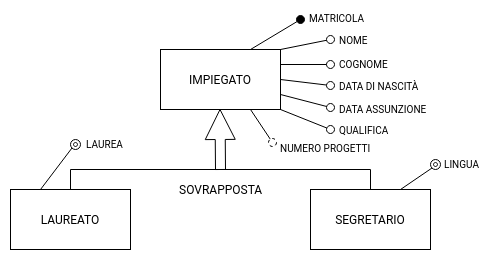
\includegraphics[width=0.5\textwidth]{er_R1.png}
\newline
\newline
Gli attributi caratteristici delle due classi di specializzazione vengono assegnati all'entità padre.
\newline
Si rinomina l'attributo laurea in tipo laurea.
\newline
\newline
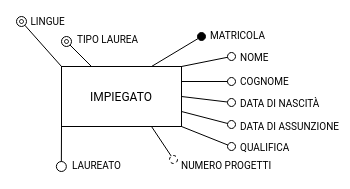
\includegraphics[width=0.5\textwidth]{er_R2.png}

\subsubsection{Eliminazione degli attributi multivalore}
É ora necessario eliminare gli attributi multivalore.
\newline
Gli unici presenti sono gli attributi "lingue" e "tipo laurea" di impiegato.
\newline
Si procede ad una reificazione.
\newline
\newline
Nel caso di tipo laurea si è deciso inoltre di separare la materia dal livello (tipo).
\newline
\newline
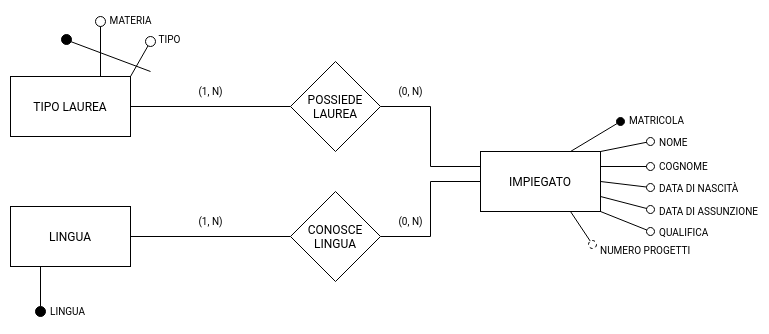
\includegraphics[width=0.5\textwidth]{er_R3.png}

\subsubsection{Eliminazione degli attributi composti}
L'unico attributo composto che compare nel diagramma ER è l'indirizzo dell'entità fornitore.
\newline
Si è scelto di scorporare il summenzionato attributo nei campi componenti.

\newpage

\subsection{Diagramma ER Ristrutturato}
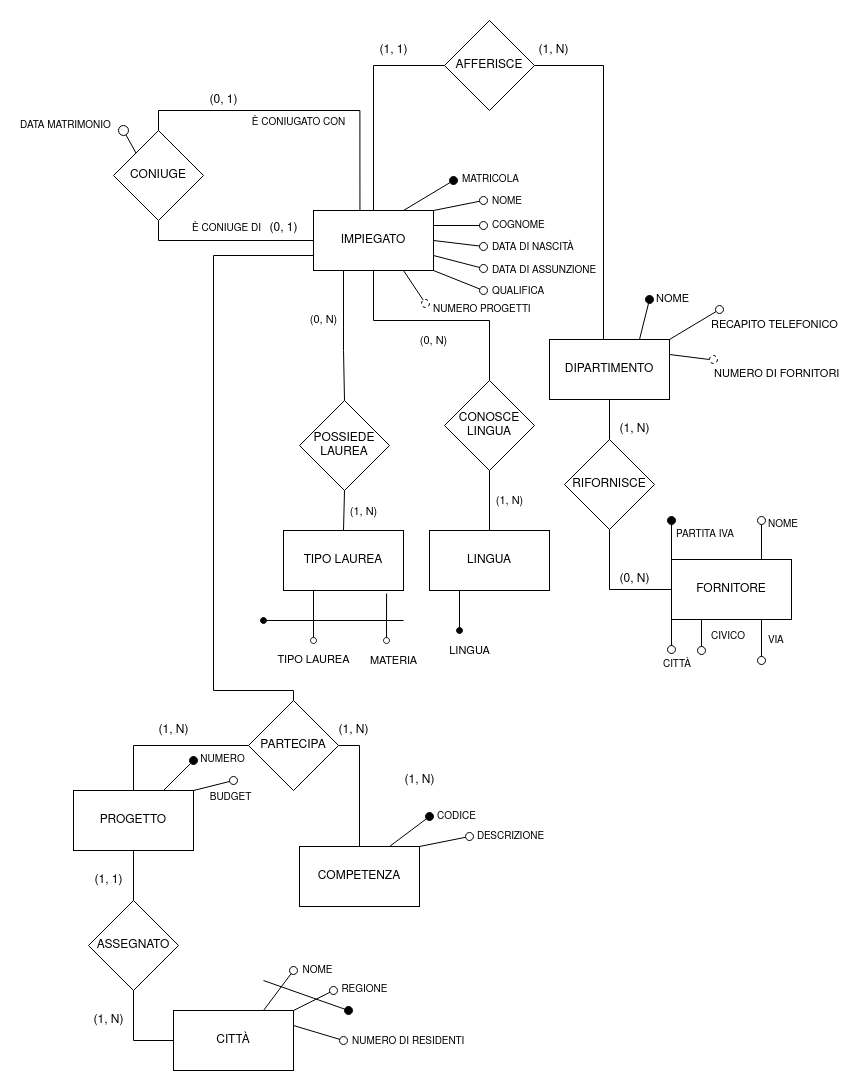
\includegraphics[width=\textwidth]{er_R.png}

\newpage

\subsection{Traduzione al modello relazionale}

\subsubsection{Traduzione delle entità}
\textbf{Fornitore} (\underline{PartitaIva}, Nome, Via, Civico, Città)
\newline
\newline
\textbf{Dipartimento} (\underline{Nome}, RecapitoTelefonico, NumeroFornitori)
\newline
- RecapitoTelefonico attributo dal valore unico
\newline
- NumeroFornitori attributo derivato
\newline
\newline
\textbf{Lingua} (\underline{Lingua})
\newline
\newline
\textbf{Impiegato} (\underline{Matricola}, Nome, Cognome, DataDiNascita, DataDiAssunzione, Dipartimento, Qualifica, NumeroProgetti)
\newline
- Dipartimento chiave esterna (riferimento alla chiave primaria dell'entità Dipartimento)
\newline
- NumeroProgetti attributo derivato
\newline
\newline
\textbf{Competenza} (\underline{Codice}, Descrizione)
\newline
- Descrizione unico
\newline
\newline
\textbf{Città} (\underline{Nome, Regione}, NumeroDiResidenti)
\newline
\newline
\textbf{Progetto} (\underline{Numero}, Budget, Città, Regione)
\newline
- Città chiave esterna (riferimento alla chiave primaria dell'entità Città)
\newline
- Regione chiave esterna (riferimento alla chiave primaria dell'entità Città)

\subsubsection{Traduzione delle relazioni}
\textbf{Rifornisce} (\underline{Dipartimento, Fornitore})
\newline
- Dipartimento chiave esterna (riferimento alla chiave primaria dell'entità Dipartimento)
\newline
- Fornitore chiave esterna (riferimento alla chiave primaria dell'entità Fornitore)
\newline
\newline
\textbf{Segretario} (\underline{Impiegato, Lingua}) [Rinomina di Conosce Lingua]
\newline
- Impiegato (riferimento alla chiave primaria dell'entità Impiegato)
\newline
- Lingua chiave esterna (riferimento alla chiave primaria dell'entità Lingua)
\newline
\newline
\textbf{Matrimonio} (\underline{Marito}, Moglie, DataDiMatrimonio) [Rinomina di Coniuge]
\newline
- Marito chieve esterna (riferimento alla chiave primaria dell'entità Impiegato)
\newline
- Moglie chieve esterna (riferimento alla chiave primaria dell'entità Impiegato)
\newline
- Moglie attributo dal valore unico
\newline
- Marito diverso da Moglie
\newline
\newline
\textbf{Laureato} (\underline{Impiegato, TipoLaurea, Materia}) [Rinomina di Possiede Laurea]
\newline
- Impiegato chiave esterna (riferimento alla chiave primaria dell'entità Impiegato)
\newline
\newline
\textbf{Partecipa} (\underline{Impiegato, Competenza, Progetto})
\newline
- Impiegato chiave esterna (riferimento alla chiave primaria dell'entità Impiegato)
\newline
- Competenza chiave esterna (riferimento alla chiave primaria dell'entità Competenza)
\newline
- Progetto chiave esterna (riferimento alla chiave primaria dell'entità Progetto)
\newline
\newline
\textbf{Afferisce}
\newline
Questa relazione uno a uno non è presente nello schema relazionale.
\newline
Si traduce nell'aggiunta dell'attributo Dipartimento all'entità Impiegato.

\newpage

\subsection{Diagramma relazionale}
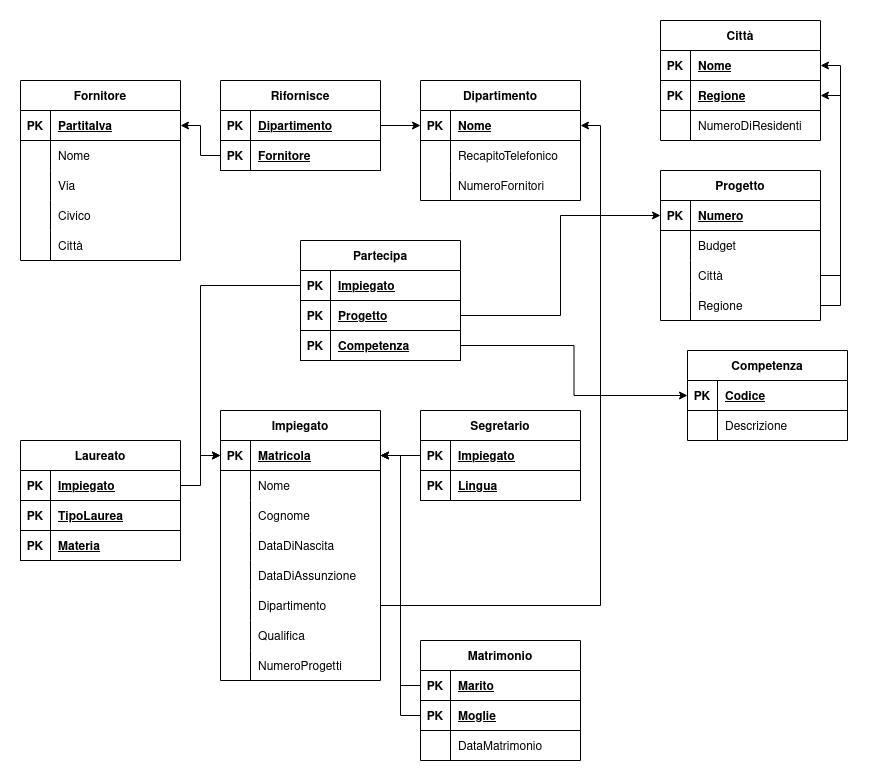
\includegraphics[width=1\textwidth]{r.png}

\subsection{Osservazioni}
Il \hyperlink{page.9}{vincolo aziendale} relativo a progetti, impiegati e città non è codificabile nello schema.
\newline
\newline
Dato che a differenza di quanto accade per gli impiegati laureati la consegna richiede che segretario sia uno dei possibili valori dell'attributo qualifica di impiegato è necessario implementare un ulteriore vincolo che garantisca che solo gli impiegati con qualifica di segretario compaiano nella tabella segretario.

\newpage

\section{Progettazione Fisica}

\subsection{Indici}
Si valuta in questa fase l'introduzione di indici per ottimizzare le prestazioni della base di dati.
\newline
\newline
Noto che le chiavi primarie e gli attributi unici delle tabelle sono già indicizzati dal DBMS PostreSQL si è ritenuto di studiare l'uso di indici sugli attributi \textbf{competenza} e \textbf{data di assunzione} della tabella \textit{\textbf{impiegato}} e sull'attributo \textbf{budget} della tabella \textit{\textbf{progetto}}.
\newline
\newline
Per valutare l'impatto degli indici sulle operazioni di lettura e scrittura si è fatto uso come tool di profiling delle interrogazioni del comando EXPLAIN ANALISE.
\newline
\newline
Tramite una semplice funzione vengono raccolti 50 tempi, con e senza indice.
\newline
Per motivi di presentazione nelle tabelle ne vengono mostrati 30 mentre tutti e 50 contribuiscono ai grafici.
\newline
A margine saranno presenti anche alcune valutazioni sulla dimensione delle tabelle.

\subsubsection{Valutazione dell'indicizzazione di qualifica di impiegato}
\textbf{Operazioni di selezione}
\begin{minted}{sql}
Interrogazione: explain analyse select * from impiegato where qualifica='Programmatore'
\end{minted}
\begin{table}[H]
\renewcommand{\arraystretch}{1.1}
\centering
\begin{tabular}{|p{4cm}|p{4cm}|p{0cm}|p{4cm}|p{4cm}|}
\cline{1-5}
Planning \textbf{senza} indice & Execution \textbf{senza} indice & & Planning \textbf{con} indice & Execution \textbf{con} indice \\ \cline{1-5}
0.048 & 0.449 & & 0.057 & 0.373 \\ \cline{1-5}
0.022 & 0.366 & & 0.029 & 0.342 \\ \cline{1-5}
0.017 & 0.299 & & 0.03 & 0.328 \\ \cline{1-5}
0.017 & 0.329 & & 0.021 & 0.285 \\ \cline{1-5}
0.017 & 0.324 & & 0.023 & 0.293 \\ \cline{1-5}
0.019 & 0.287 & & 0.028 & 0.31 \\ \cline{1-5}
0.02 & 0.318 & & 0.028 & 0.282 \\ \cline{1-5}
0.035 & 0.367 & & 0.02 & 0.285 \\ \cline{1-5}
0.019 & 0.299 & & 0.022 & 0.337 \\ \cline{1-5}
0.023 & 0.344 & & 0.03 & 0.287 \\ \cline{1-5}
0.018 & 0.304 & & 0.028 & 0.291 \\ \cline{1-5}
0.045 & 0.494 & & 0.029 & 0.288 \\ \cline{1-5}
0.023 & 0.344 & & 0.059 & 0.431 \\ \cline{1-5}
0.02 & 0.333 & & 0.033 & 0.312 \\ \cline{1-5}
0.02 & 0.313 & & 0.021 & 0.288 \\ \cline{1-5}
0.026 & 0.302 & & 0.02 & 0.292 \\ \cline{1-5}
0.025 & 0.317 & & 0.029 & 0.307 \\ \cline{1-5}
0.017 & 0.285 & & 0.028 & 0.28 \\ \cline{1-5}
0.017 & 0.283 & & 0.02 & 0.288 \\ \cline{1-5}
0.017 & 0.279 & & 0.023 & 0.31 \\ \cline{1-5}
0.016 & 0.278 & & 0.031 & 0.294 \\ \cline{1-5}
0.017 & 0.277 & & 0.02 & 0.29 \\ \cline{1-5}
0.017 & 0.311 & & 0.026 & 0.29 \\ \cline{1-5}
0.017 & 0.284 & & 0.029 & 0.285 \\ \cline{1-5}
0.016 & 0.277 & & 0.02 & 0.291 \\ \cline{1-5}
0.017 & 0.306 & & 0.02 & 0.288 \\ \cline{1-5}
0.023 & 0.27 & & 0.021 & 0.306 \\ \cline{1-5}
0.047 & 0.433 & & 0.02 & 0.293 \\ \cline{1-5}
0.029 & 0.365 & & 0.021 & 0.289 \\ \cline{1-5}
0.021 & 0.367 & & 0.027 & 0.303 \\ \cline{1-5}
\end{tabular}
\end{table}

\newpage
\noindent
\textbf{Operazioni di modifica}
\begin{minted}{sql}
Interrogazione:
explain analyse update impiegato set qualifica='Analista' where numero_progetti between 2 and 3
\end{minted}
\begin{table}[H]
\renewcommand{\arraystretch}{1.1}
\centering
\begin{tabular}{|p{4cm}|p{4cm}|p{0cm}|p{4cm}|p{4cm}|}
\cline{1-5}
Planning \textbf{senza} indice & Execution \textbf{senza} indice & & Planning \textbf{con} indice & Execution \textbf{con} indice \\ \cline{1-5}
0.07 & 5.044 & & 0.072 & 4.841 \\ \cline{1-5}
0.069 & 6.875 & & 0.074 & 4.988 \\ \cline{1-5}
0.064 & 5.414 & & 0.062 & 4.992 \\ \cline{1-5}
0.094 & 6.242 & & 0.065 & 4.801 \\ \cline{1-5}
0.067 & 4.806 & & 0.111 & 5.125 \\ \cline{1-5}
0.086 & 4.958 & & 0.055 & 5.225 \\ \cline{1-5}
0.058 & 4.586 & & 0.046 & 4.821 \\ \cline{1-5}
0.04 & 4.538 & & 0.143 & 5.447 \\ \cline{1-5}
0.077 & 5.114 & & 0.086 & 5.777 \\ \cline{1-5}
0.049 & 4.981 & & 0.077 & 5.946 \\ \cline{1-5}
0.065 & 4.731 & & 0.058 & 5.284 \\ \cline{1-5}
0.048 & 4.92 & & 0.051 & 5.815 \\ \cline{1-5}
0.065 & 4.819 & & 0.152 & 5.433 \\ \cline{1-5}
0.042 & 4.507 & & 0.071 & 5.827 \\ \cline{1-5}
0.043 & 4.755 & & 0.05 & 5.552 \\ \cline{1-5}
0.035 & 4.589 & & 0.041 & 5.236 \\ \cline{1-5}
0.039 & 4.669 & & 0.05 & 5.247 \\ \cline{1-5}
0.043 & 4.574 & & 0.049 & 5.308 \\ \cline{1-5}
0.032 & 4.493 & & 0.05 & 5.039 \\ \cline{1-5}
0.039 & 4.474 & & 0.045 & 5.247 \\ \cline{1-5}
0.04 & 4.771 & & 0.035 & 5.23 \\ \cline{1-5}
0.04 & 4.49 & & 0.059 & 5.107 \\ \cline{1-5}
0.031 & 4.547 & & 0.036 & 4.863 \\ \cline{1-5}
0.031 & 4.625 & & 0.033 & 5.094 \\ \cline{1-5}
0.031 & 4.571 & & 0.035 & 4.873 \\ \cline{1-5}
0.039 & 4.441 & & 0.033 & 4.976 \\ \cline{1-5}
0.04 & 4.622 & & 0.033 & 4.998 \\ \cline{1-5}
0.041 & 4.485 & & 0.033 & 4.88 \\ \cline{1-5}
0.032 & 4.657 & & 0.033 & 4.853 \\ \cline{1-5}
0.043 & 4.61 & & 0.044 & 5.175 \\ \cline{1-5}
\end{tabular}
\end{table}
\noindent
\newline
\textbf{Considerazioni sullo spazio occupato}
\newline
\newline
Sfruttando le seguenti interrogazioni è possibile conoscere lo spazio occupato dalla tabella e dagli indici:
\begin{minted}{sql}
SELECT pg_size_pretty(pg_total_relation_size ('impiegato'));
SELECT pg_size_pretty(pg_indexes_size ('impiegato'));
\end{minted}
Per impiegato il risultato è di \textbf{2128kB} prima dell'indicizzazione e \textbf{2224kB} a seguito di essa con una dimensione dell'indice di \textbf{96kB}.

\newpage
\noindent
\newline
Concludiamo visualizzando i risultati della profilazione tramite box plot realizzati in R:
\newline
\newline
\textbf{Operazioni di selezione}
\newline
\newline
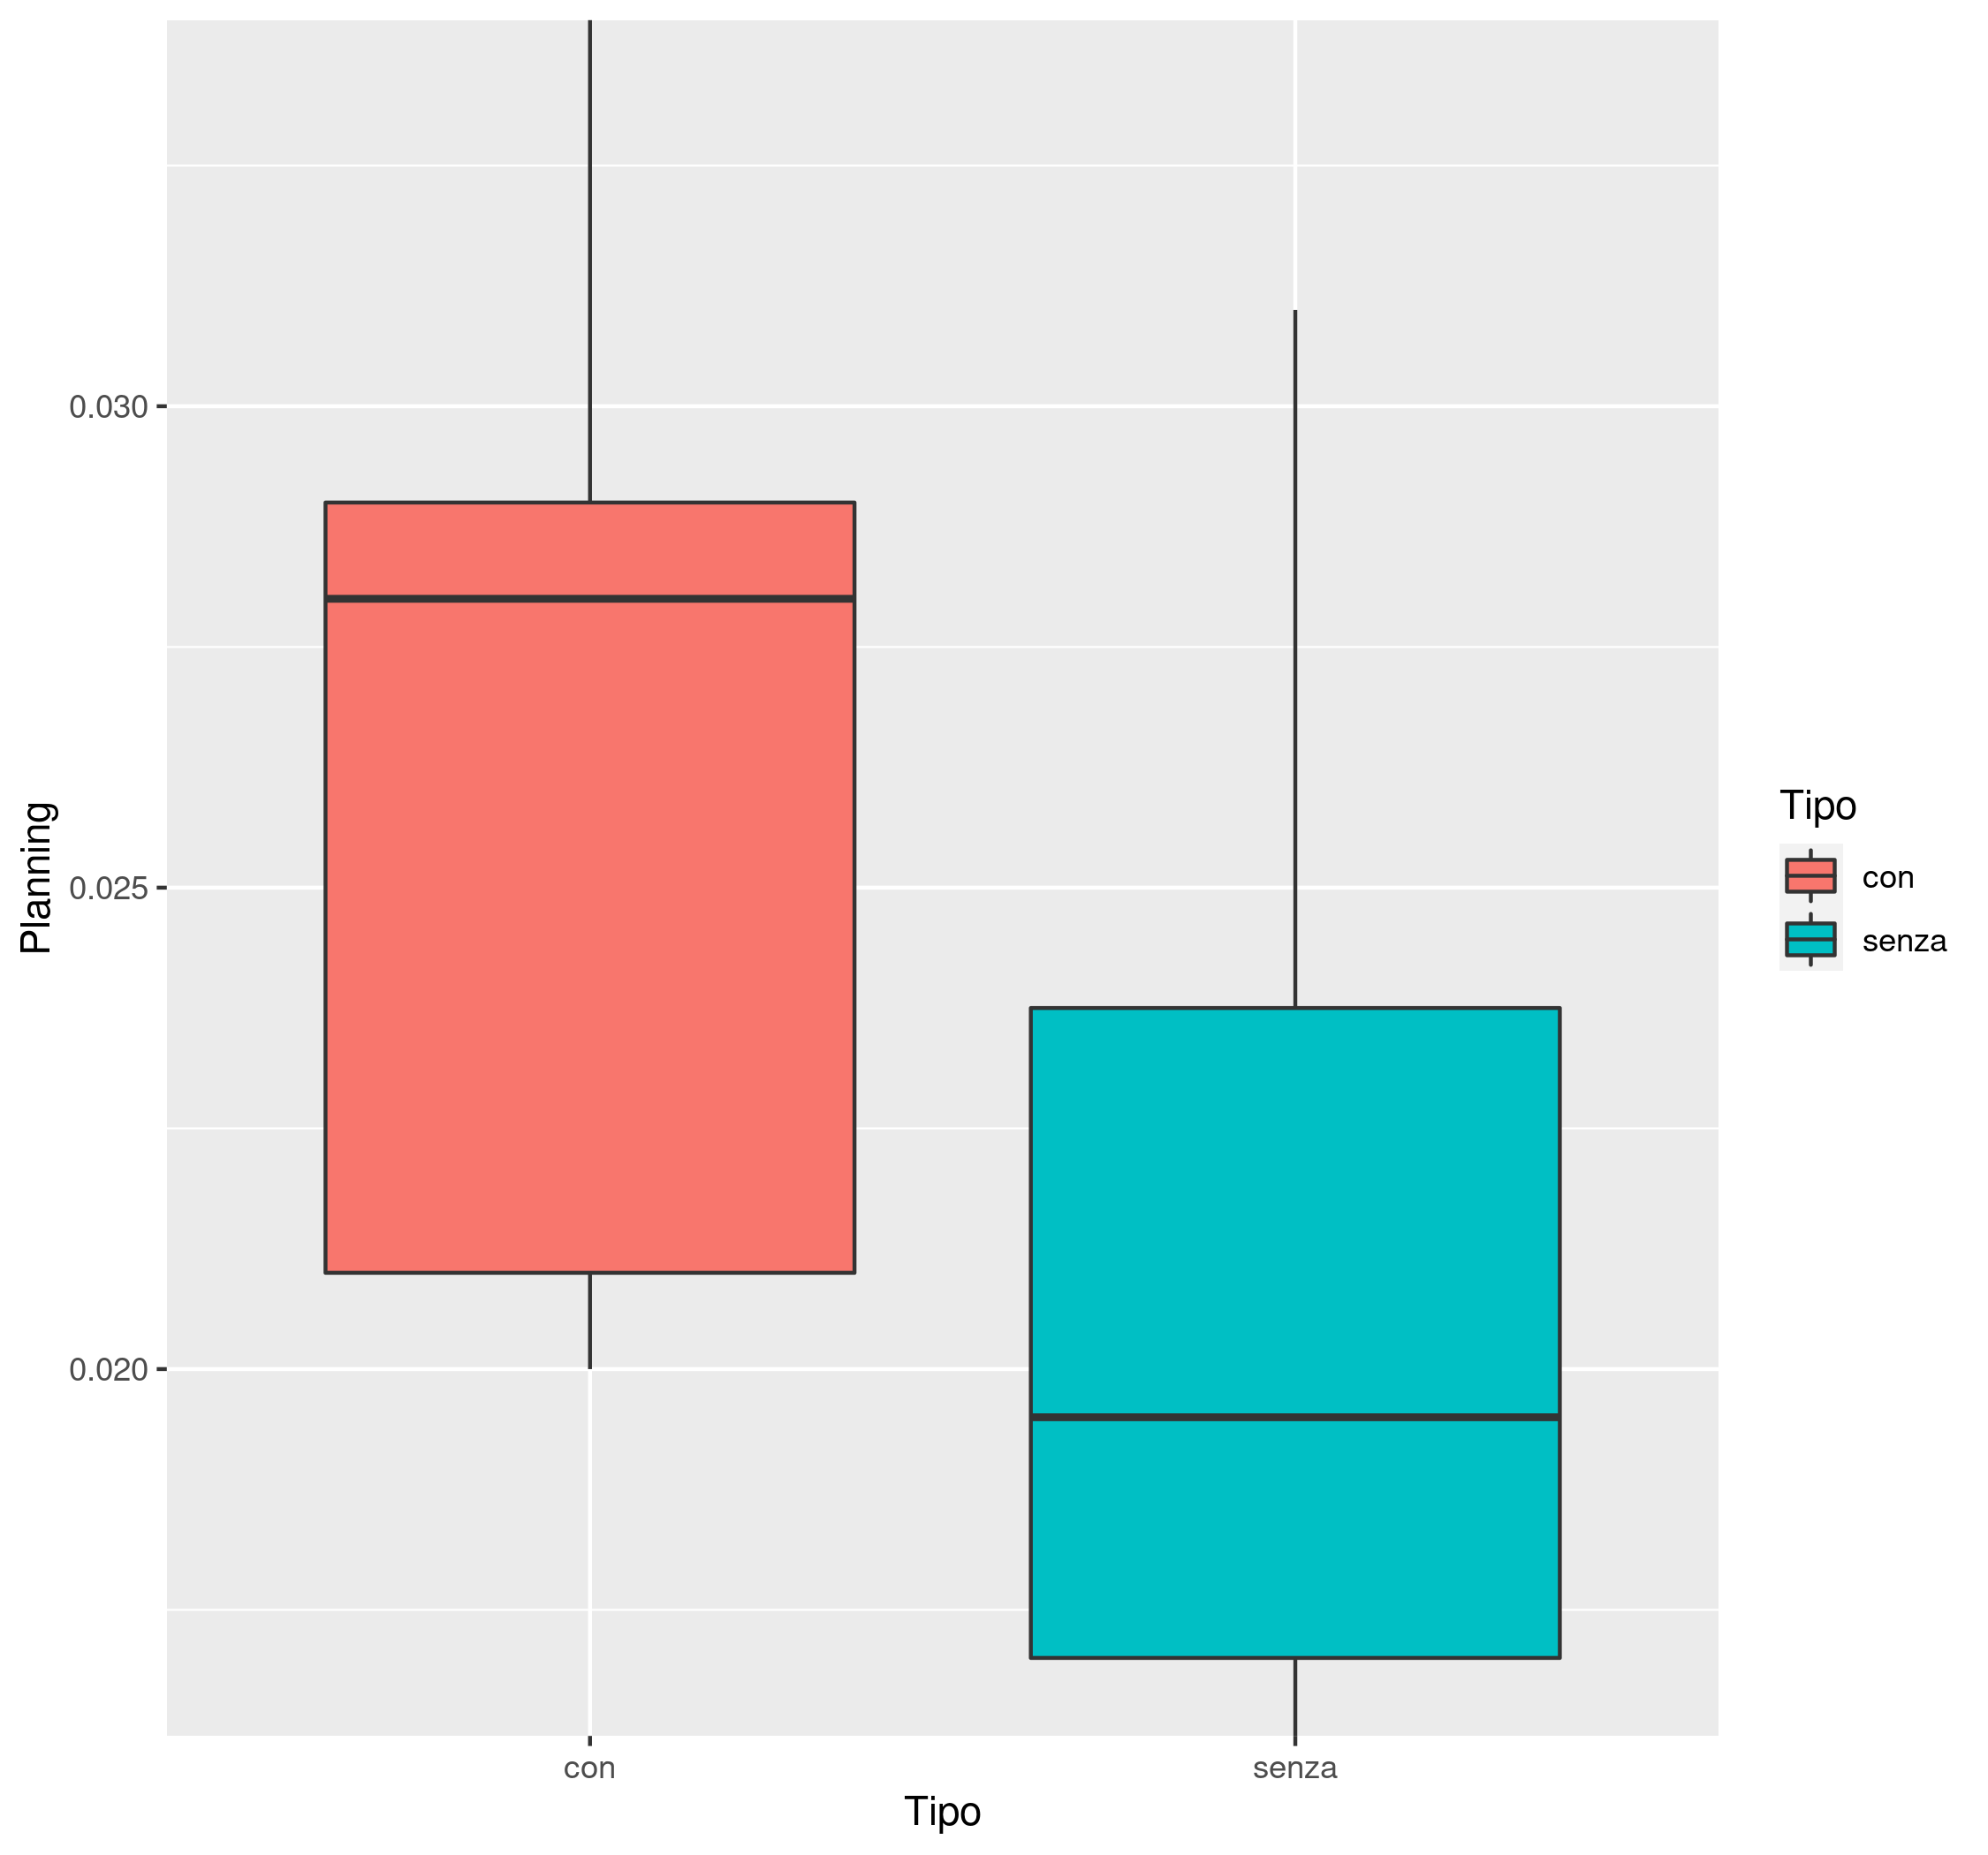
\includegraphics[width=0.5\textwidth]{planning_impiegato_qualifica_selezione.png}
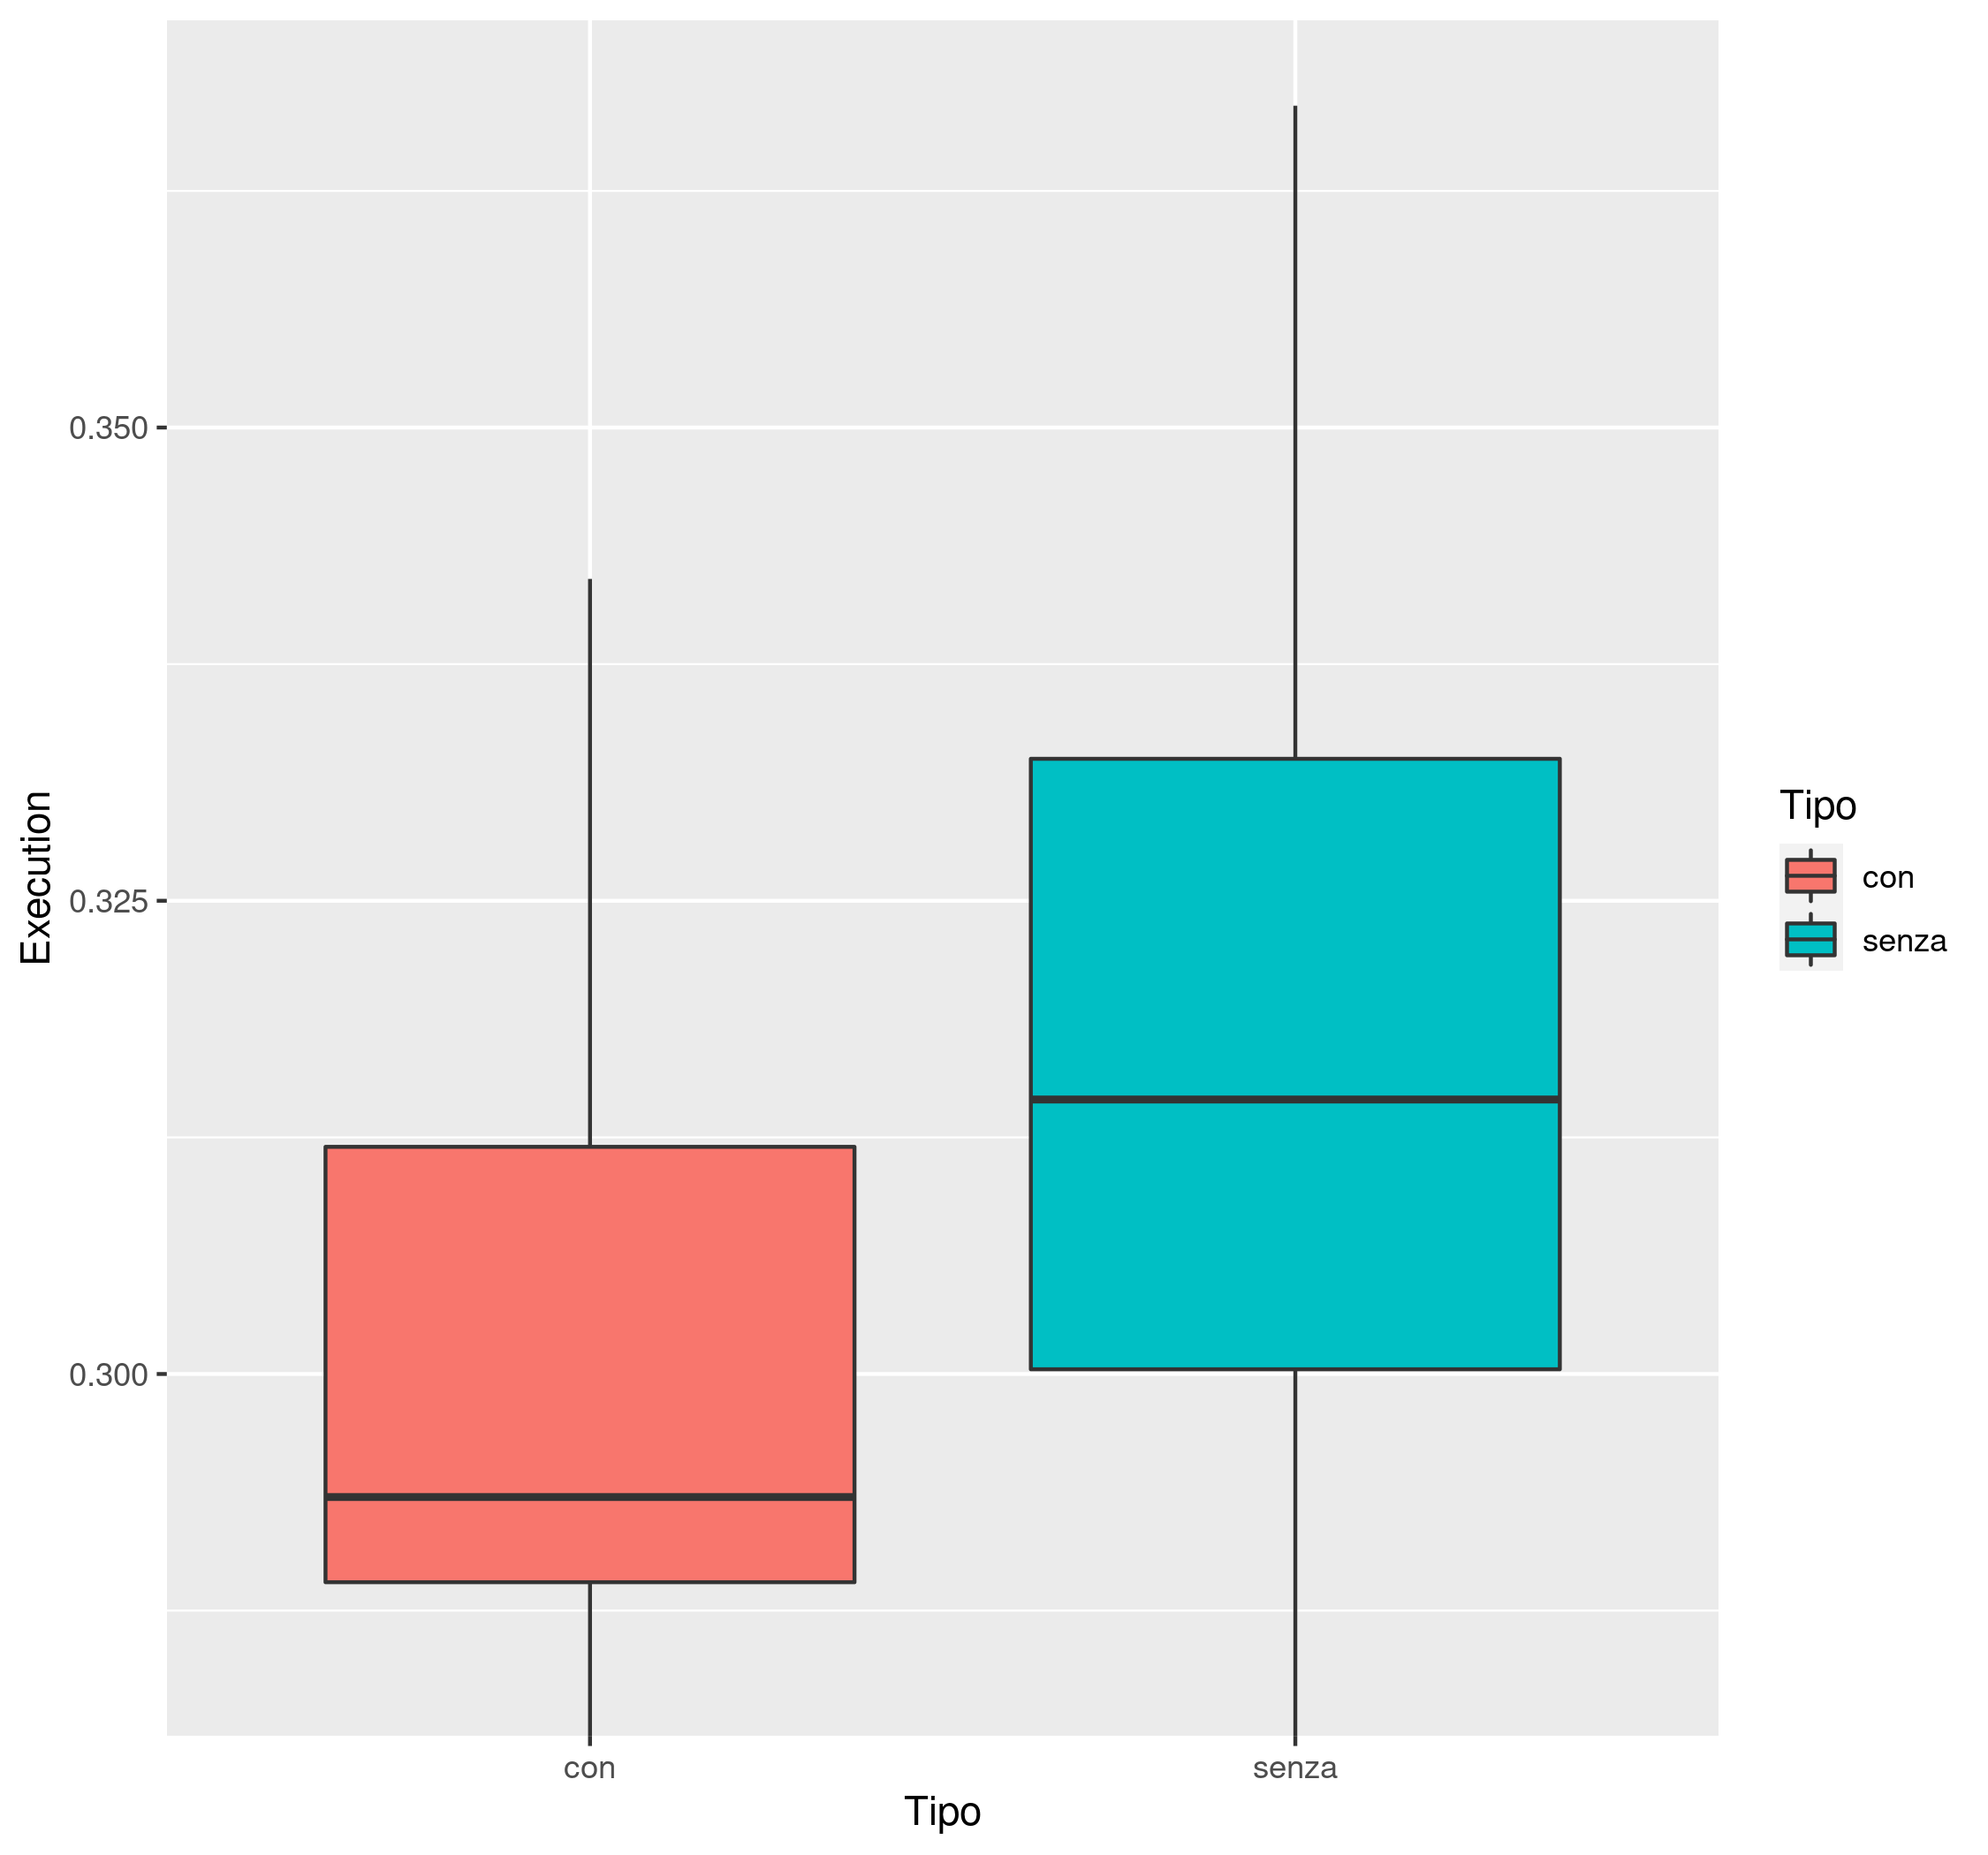
\includegraphics[width=0.5\textwidth]{execution_impiegato_qualifica_selezione.png}
\newline
\newline
\textbf{Operazioni di modifica}
\newline
\newline
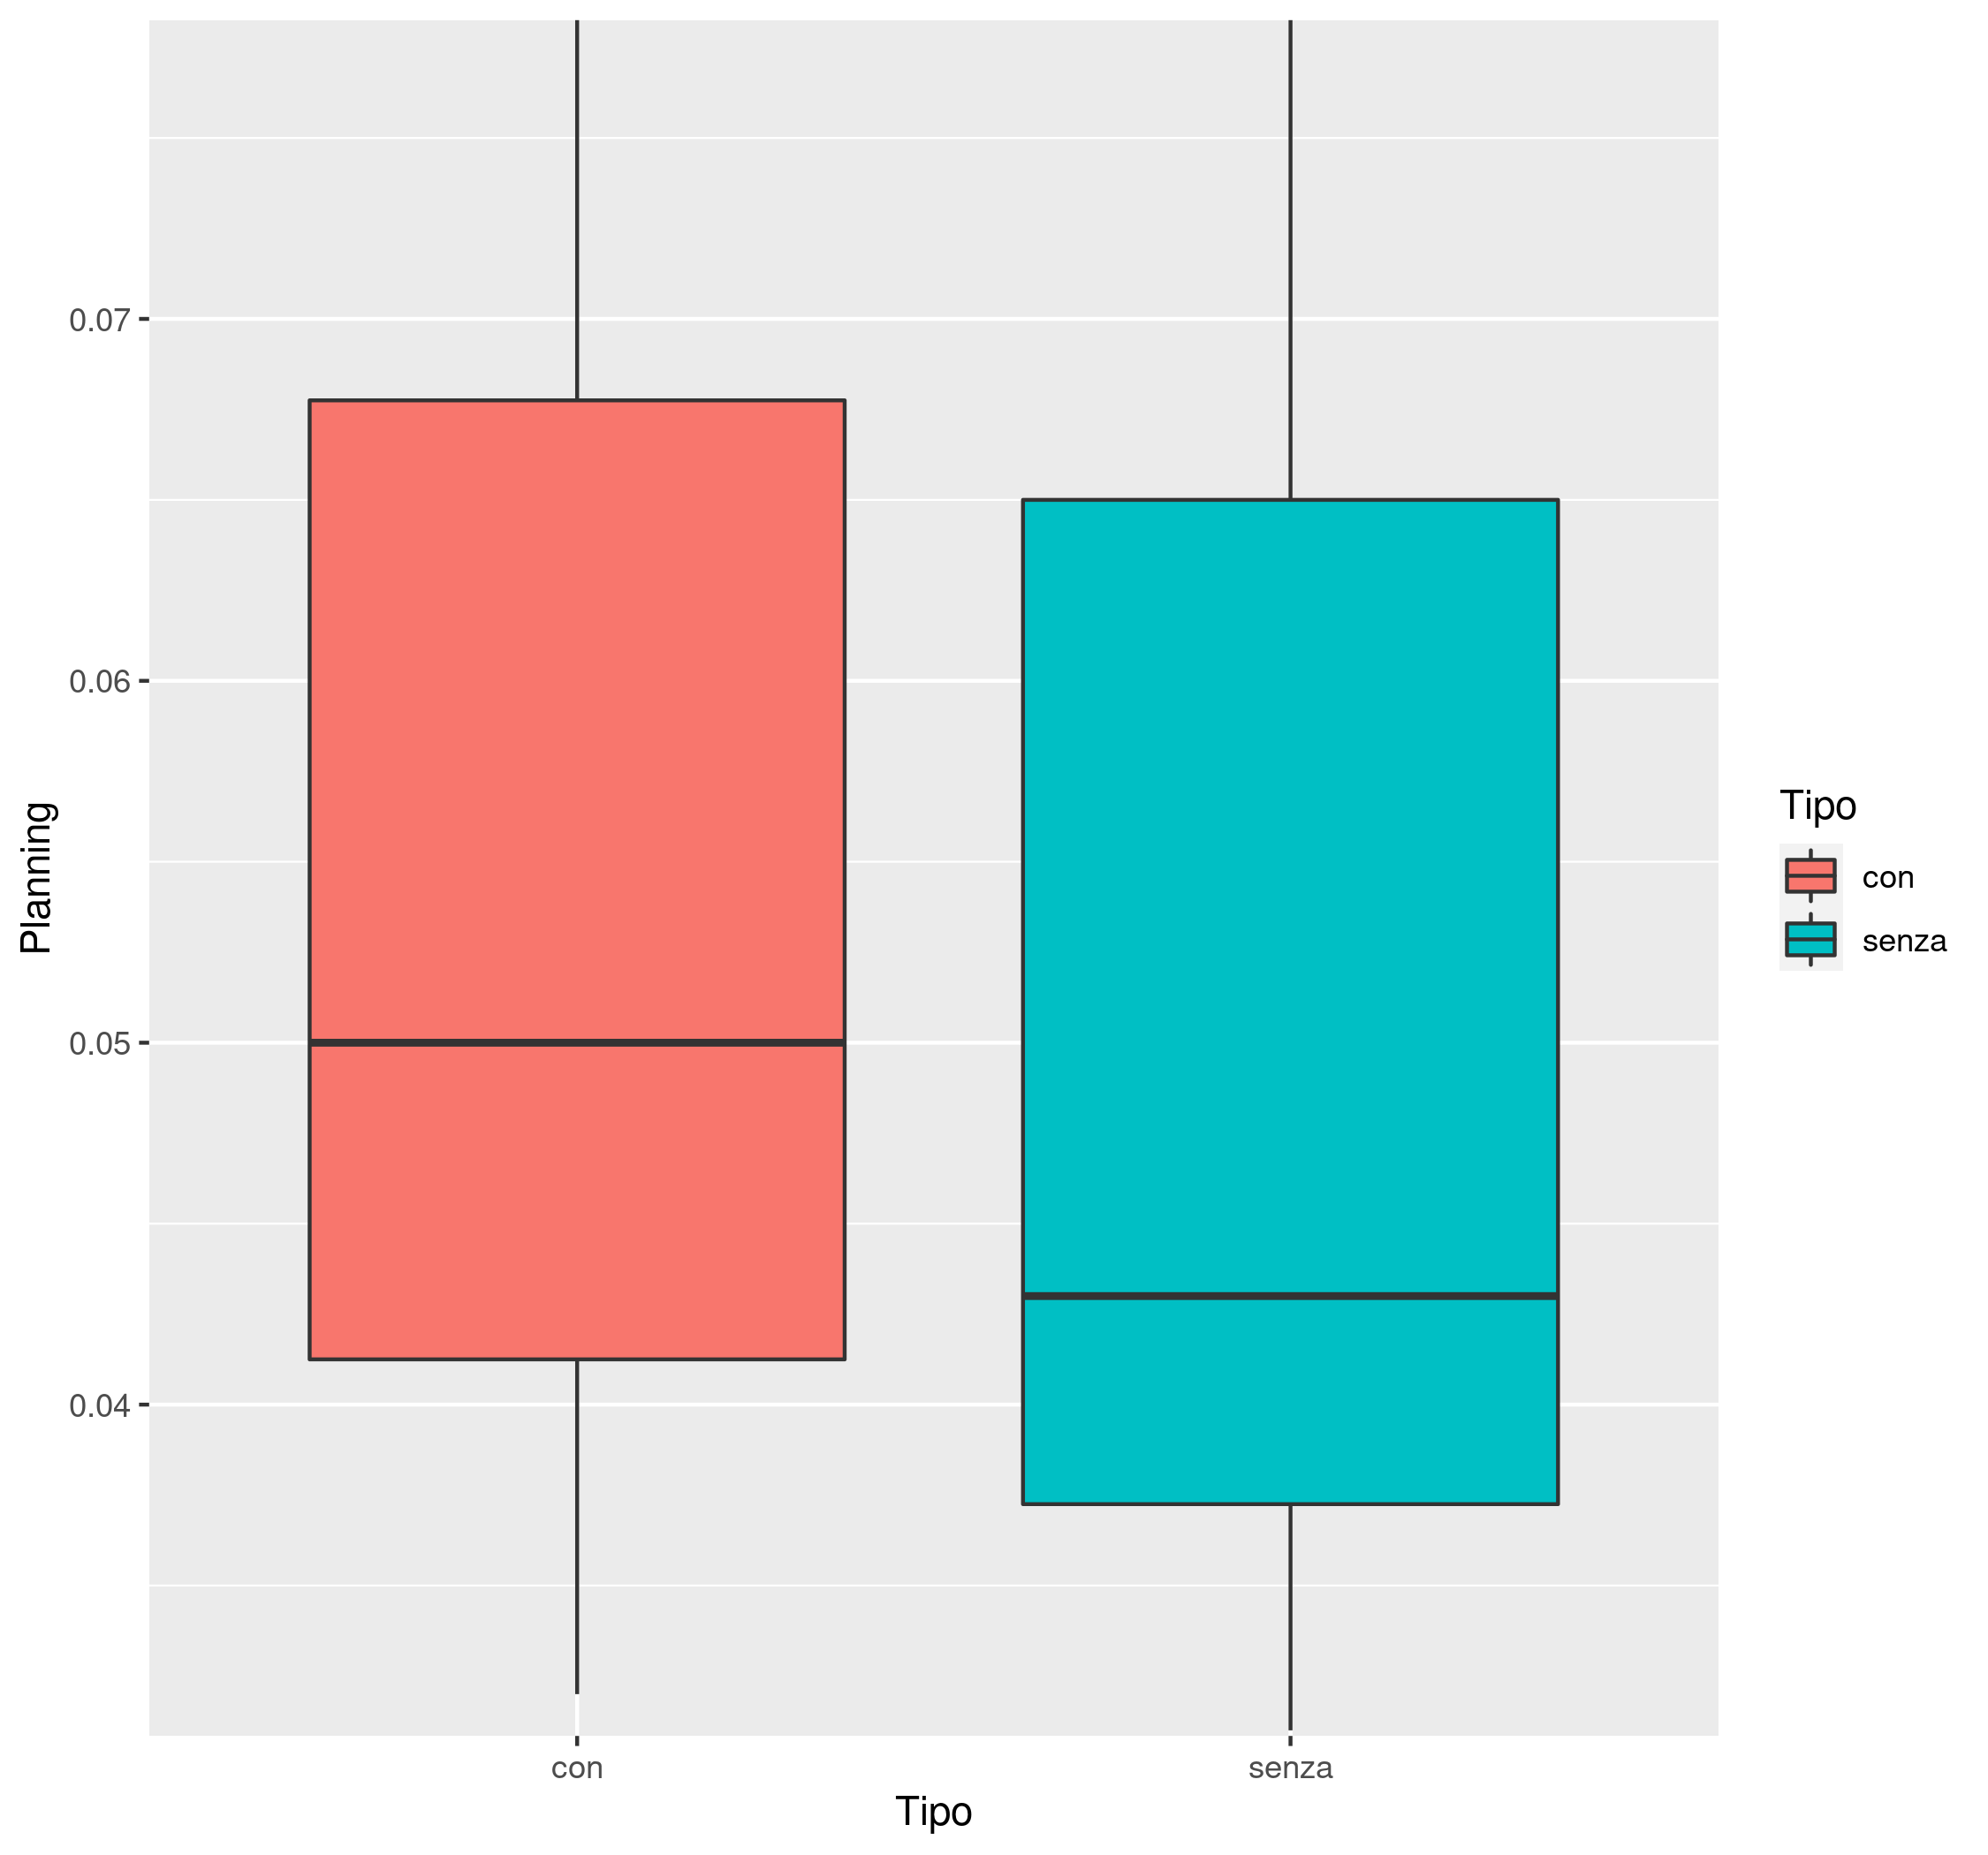
\includegraphics[width=0.5\textwidth]{planning_impiegato_qualifica_modifica.png}
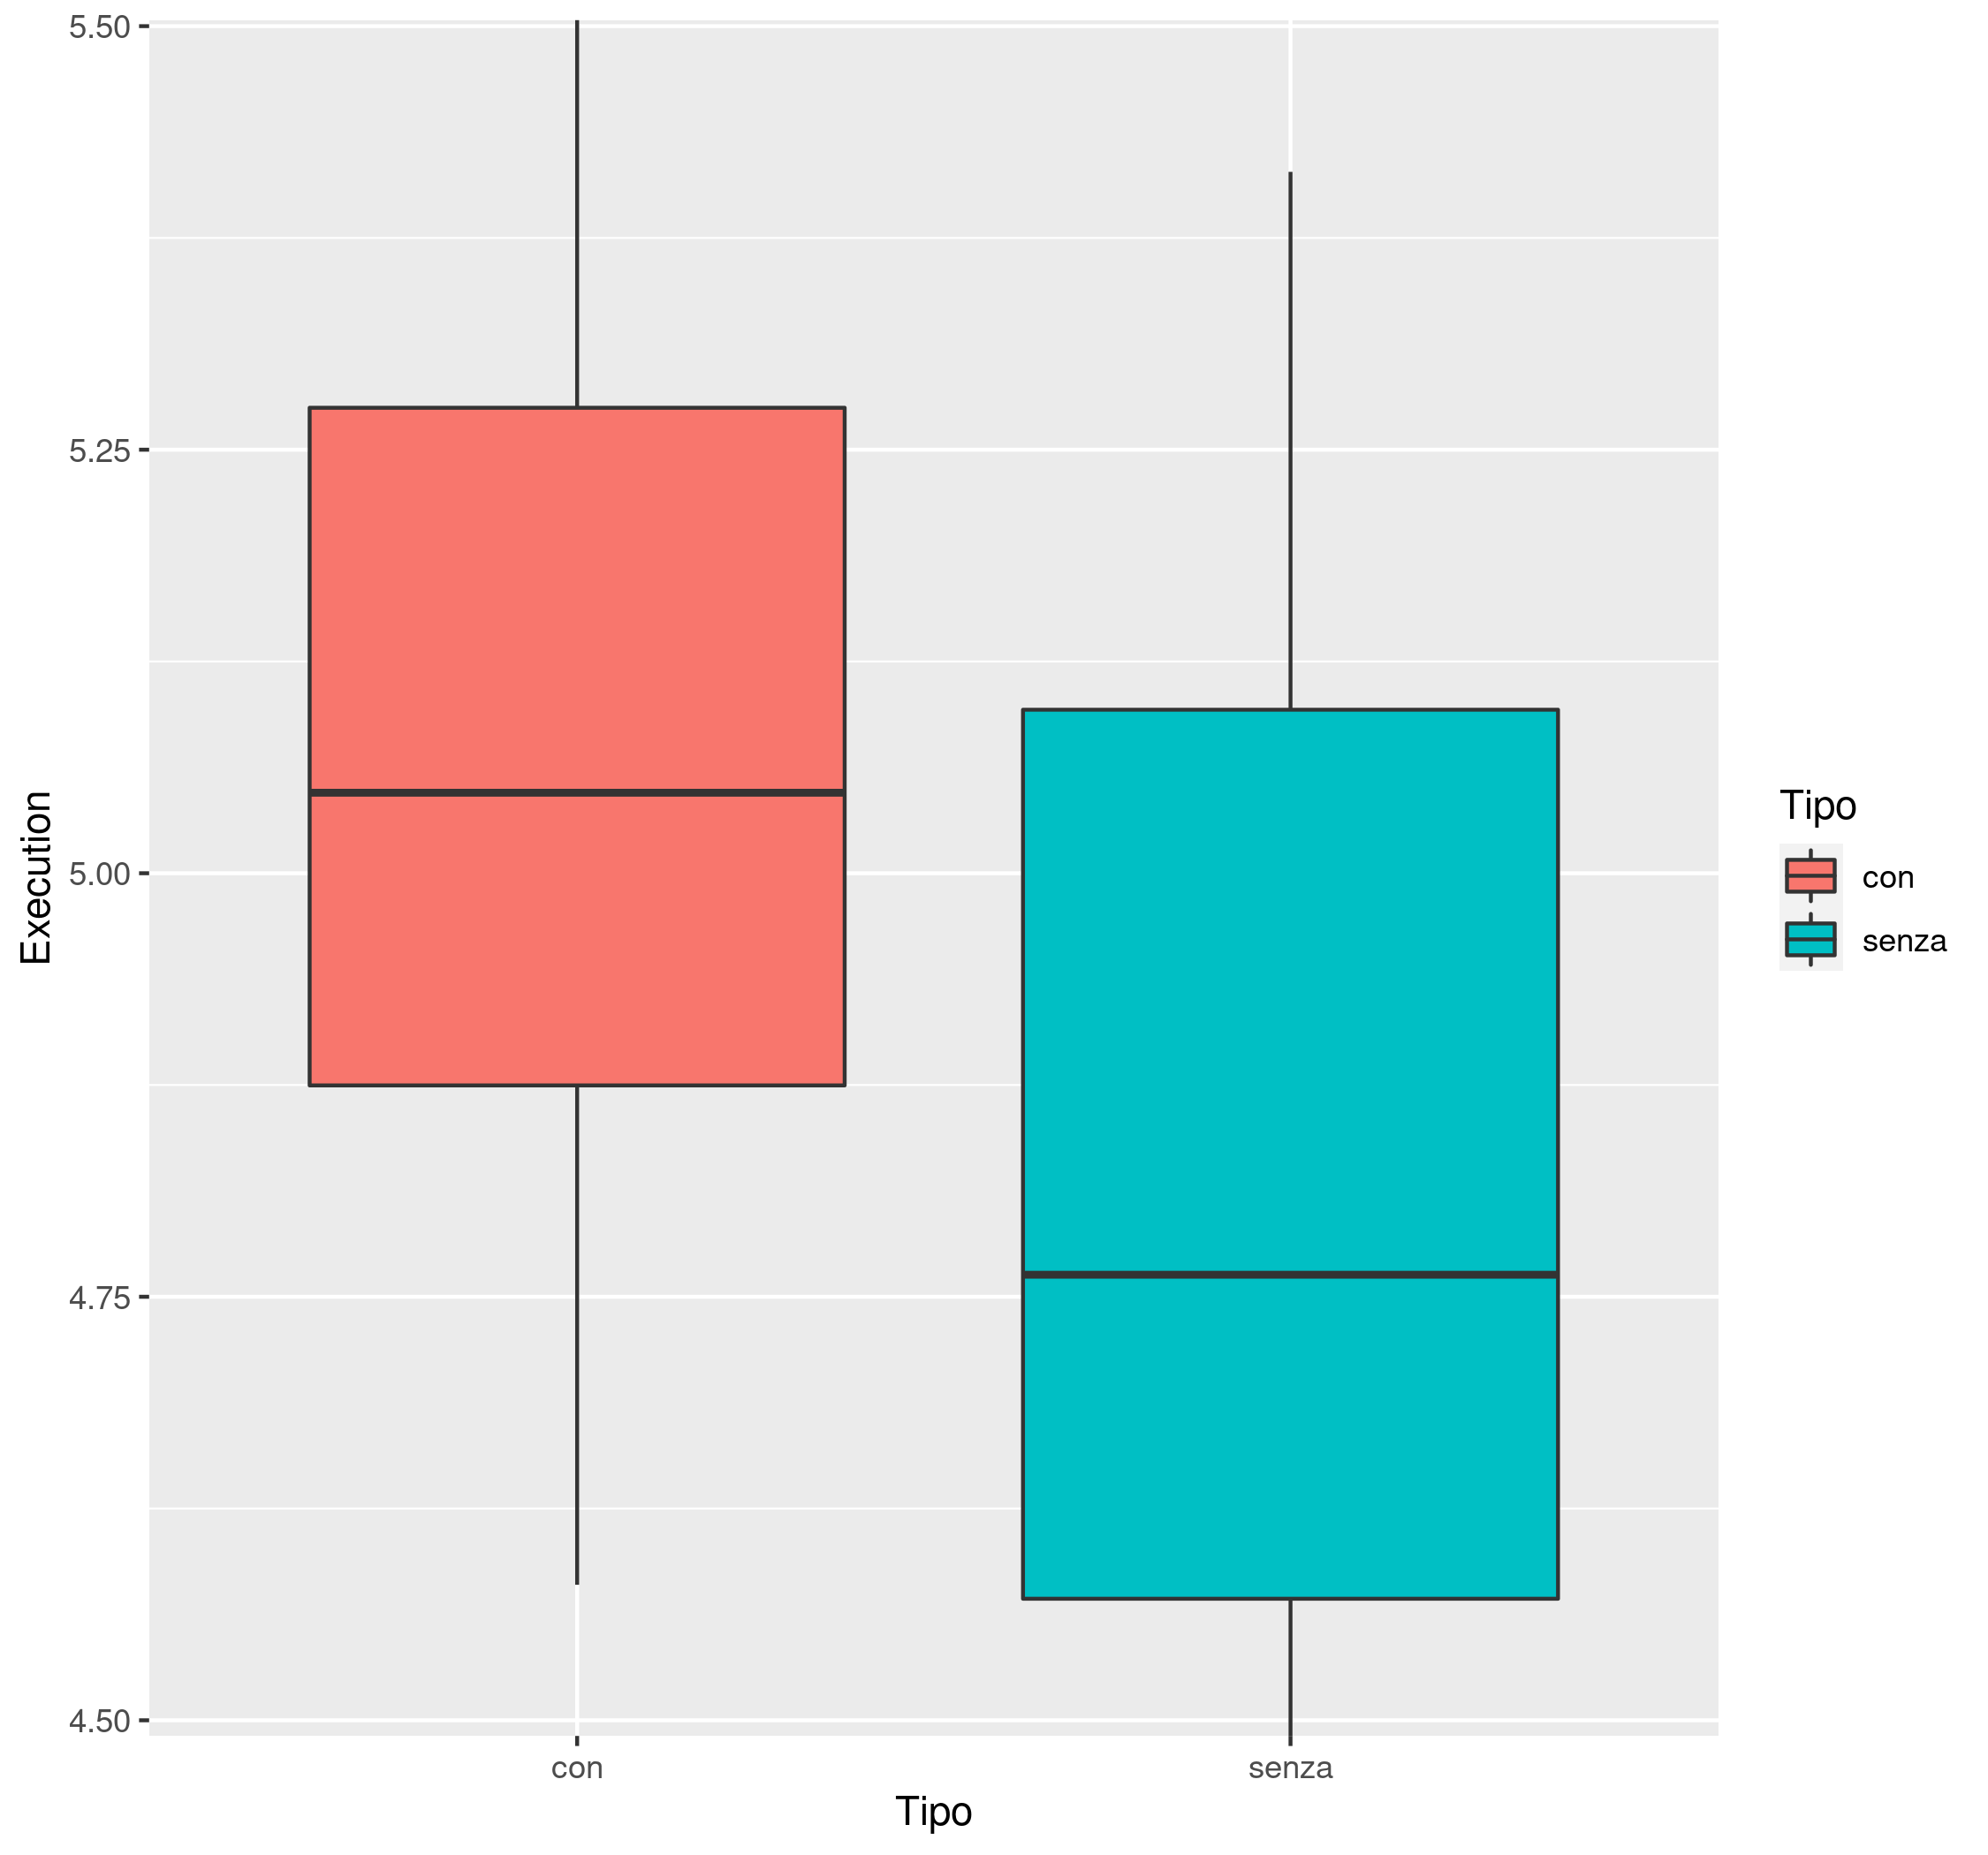
\includegraphics[width=0.5\textwidth]{execution_impiegato_qualifica_modifica.png}
\newline
\newline
Visto l'esito del profiling e data la natura dell'attributo su cui si è costruito l'indice si ritiene di implementarlo.

\newpage

\subsubsection{Valutazione dell'indicizzazione di data di assunzione di impiegato}
\textbf{Operazioni di selezione}
\begin{minted}{sql}
Interrogazione: explain analyse select * from impiegato where data_di_assunzione<='20000101'
\end{minted}
\begin{table}[H]
\renewcommand{\arraystretch}{1.1}
\centering
\begin{tabular}{|p{4cm}|p{4cm}|p{0cm}|p{4cm}|p{4cm}|}
\cline{1-5}
Planning \textbf{senza} indice & Execution \textbf{senza} indice & & Planning \textbf{con} indice & Execution \textbf{con} indice \\ \cline{1-5}
0.084 & 0.896 & & 0.092 & 0.014 \\ \cline{1-5}
0.04 & 0.778 & & 0.053 & 0.019 \\ \cline{1-5}
0.026 & 0.356 & & 0.06 & 0.01 \\ \cline{1-5}
0.036 & 0.377 & & 0.061 & 0.01 \\ \cline{1-5}
0.024 & 0.33 & & 0.061 & 0.01 \\ \cline{1-5}
0.036 & 0.338 & & 0.059 & 0.01 \\ \cline{1-5}
0.052 & 0.452 & & 0.064 & 0.012 \\ \cline{1-5}
0.026 & 0.548 & & 0.068 & 0.011 \\ \cline{1-5}
0.116 & 1.23 & & 0.117 & 0.014 \\ \cline{1-5}
0.054 & 0.471 & & 0.08 & 0.012 \\ \cline{1-5}
0.03 & 0.324 & & 0.061 & 0.01 \\ \cline{1-5}
0.028 & 0.293 & & 0.081 & 0.027 \\ \cline{1-5}
0.018 & 0.277 & & 0.061 & 0.011 \\ \cline{1-5}
0.019 & 0.294 & & 0.09 & 0.029 \\ \cline{1-5}
0.018 & 0.271 & & 0.072 & 0.013 \\ \cline{1-5}
0.029 & 0.386 & & 0.06 & 0.01 \\ \cline{1-5}
0.019 & 0.27 & & 0.059 & 0.011 \\ \cline{1-5}
0.036 & 0.465 & & 0.112 & 0.021 \\ \cline{1-5}
0.02 & 0.331 & & 0.089 & 0.022 \\ \cline{1-5}
0.03 & 0.316 & & 0.065 & 0.011 \\ \cline{1-5}
0.04 & 0.524 & & 0.064 & 0.014 \\ \cline{1-5}
0.027 & 0.366 & & 0.103 & 0.013 \\ \cline{1-5}
0.033 & 0.539 & & 0.107 & 0.015 \\ \cline{1-5}
0.029 & 0.341 & & 0.095 & 0.023 \\ \cline{1-5}
0.027 & 0.352 & & 0.046 & 0.01 \\ \cline{1-5}
0.037 & 0.317 & & 0.051 & 0.009 \\ \cline{1-5}
0.034 & 0.384 & & 0.076 & 0.01 \\ \cline{1-5}
0.052 & 0.45 & & 0.075 & 0.016 \\ \cline{1-5}
0.027 & 0.428 & & 0.071 & 0.012 \\ \cline{1-5}
0.045 & 0.711 & & 0.08 & 0.012 \\ \cline{1-5}
\end{tabular}
\end{table}

\newpage
\noindent
\textbf{Operazioni di modifica}
\begin{minted}{sql}
Interrogazione:
explain analyse 
    update impiegato 
        set data_di_assunzione='20220829' where data_di_nascita between '19820101' and '20050101'
\end{minted}
\begin{table}[H]
\renewcommand{\arraystretch}{1.2}
\centering
\begin{tabular}{|p{4cm}|p{4cm}|p{0cm}|p{4cm}|p{4cm}|}
\cline{1-5}
Planning \textbf{senza} indice & Execution \textbf{senza} indice & & Planning \textbf{con} indice & Execution \textbf{con} indice \\ \cline{1-5}
0.069 & 7.221 & & 0.073 & 7.519 \\ \cline{1-5}
0.143 & 7.546 & & 0.066 & 6.17 \\ \cline{1-5}
0.097 & 7.623 & & 0.055 & 6.281 \\ \cline{1-5}
0.124 & 7.475 & & 0.107 & 7.559 \\ \cline{1-5}
0.072 & 7.268 & & 0.068 & 7.164 \\ \cline{1-5}
0.068 & 7.978 & & 0.072 & 6.133 \\ \cline{1-5}
0.113 & 12.945 & & 0.101 & 6.604 \\ \cline{1-5}
0.065 & 6.818 & & 0.051 & 6.122 \\ \cline{1-5}
0.046 & 6.371 & & 0.046 & 6.782 \\ \cline{1-5}
0.043 & 6.328 & & 0.048 & 6.263 \\ \cline{1-5}
0.044 & 6.414 & & 0.035 & 6.486 \\ \cline{1-5}
0.074 & 8.316 & & 0.037 & 6.531 \\ \cline{1-5}
0.081 & 6.918 & & 0.037 & 6.479 \\ \cline{1-5}
0.062 & 7.582 & & 0.047 & 6.468 \\ \cline{1-5}
0.081 & 6.874 & & 0.036 & 6.444 \\ \cline{1-5}
0.046 & 6.597 & & 0.034 & 6.547 \\ \cline{1-5}
0.037 & 6.201 & & 0.049 & 6.548 \\ \cline{1-5}
0.046 & 6.235 & & 0.043 & 6.966 \\ \cline{1-5}
0.083 & 4.914 & & 0.071 & 6.882 \\ \cline{1-5}
0.029 & 4.792 & & 0.084 & 6.668 \\ \cline{1-5}
0.028 & 4.691 & & 0.083 & 6.987 \\ \cline{1-5}
0.027 & 4.609 & & 0.098 & 6.878 \\ \cline{1-5}
0.034 & 4.585 & & 0.08 & 6.891 \\ \cline{1-5}
0.035 & 4.651 & & 0.079 & 6.878 \\ \cline{1-5}
0.026 & 4.521 & & 0.072 & 7.138 \\ \cline{1-5}
0.035 & 4.61 & & 0.091 & 7.488 \\ \cline{1-5}
0.035 & 4.653 & & 0.069 & 7.252 \\ \cline{1-5}
0.045 & 5.002 & & 0.072 & 6.607 \\ \cline{1-5}
0.029 & 4.568 & & 0.073 & 6.82 \\ \cline{1-5}
0.052 & 5.783 & & 0.118 & 7.071 \\ \cline{1-5}
\end{tabular}
\end{table}
\noindent
\newline
\textbf{Considerazioni sullo spazio occupato}
\newline
\newline
Sfruttando le seguenti interrogazioni è possibile conoscere lo spazio occupato dalla tabella e dagli indici:
\begin{minted}{sql}
SELECT pg_size_pretty(pg_total_relation_size ('impiegato'));
SELECT pg_size_pretty(pg_indexes_size ('impiegato'));
\end{minted}
Per impiegato il risultato è di \textbf{2224kB} prima dell'indicizzazione e \textbf{2312kB} a seguito di essa con una dimensione dell'indice di \textbf{88kB}.

\newpage
\noindent
\newline
Concludiamo visualizzando i risultati della profilazione tramite box plot realizzati in R:
\newline
\newline
\textbf{Operazioni di selezione}
\newline
\newline
\includegraphics[width=0.5\textwidth]{planning_impiegato_dataAssunzione_selezione.png}
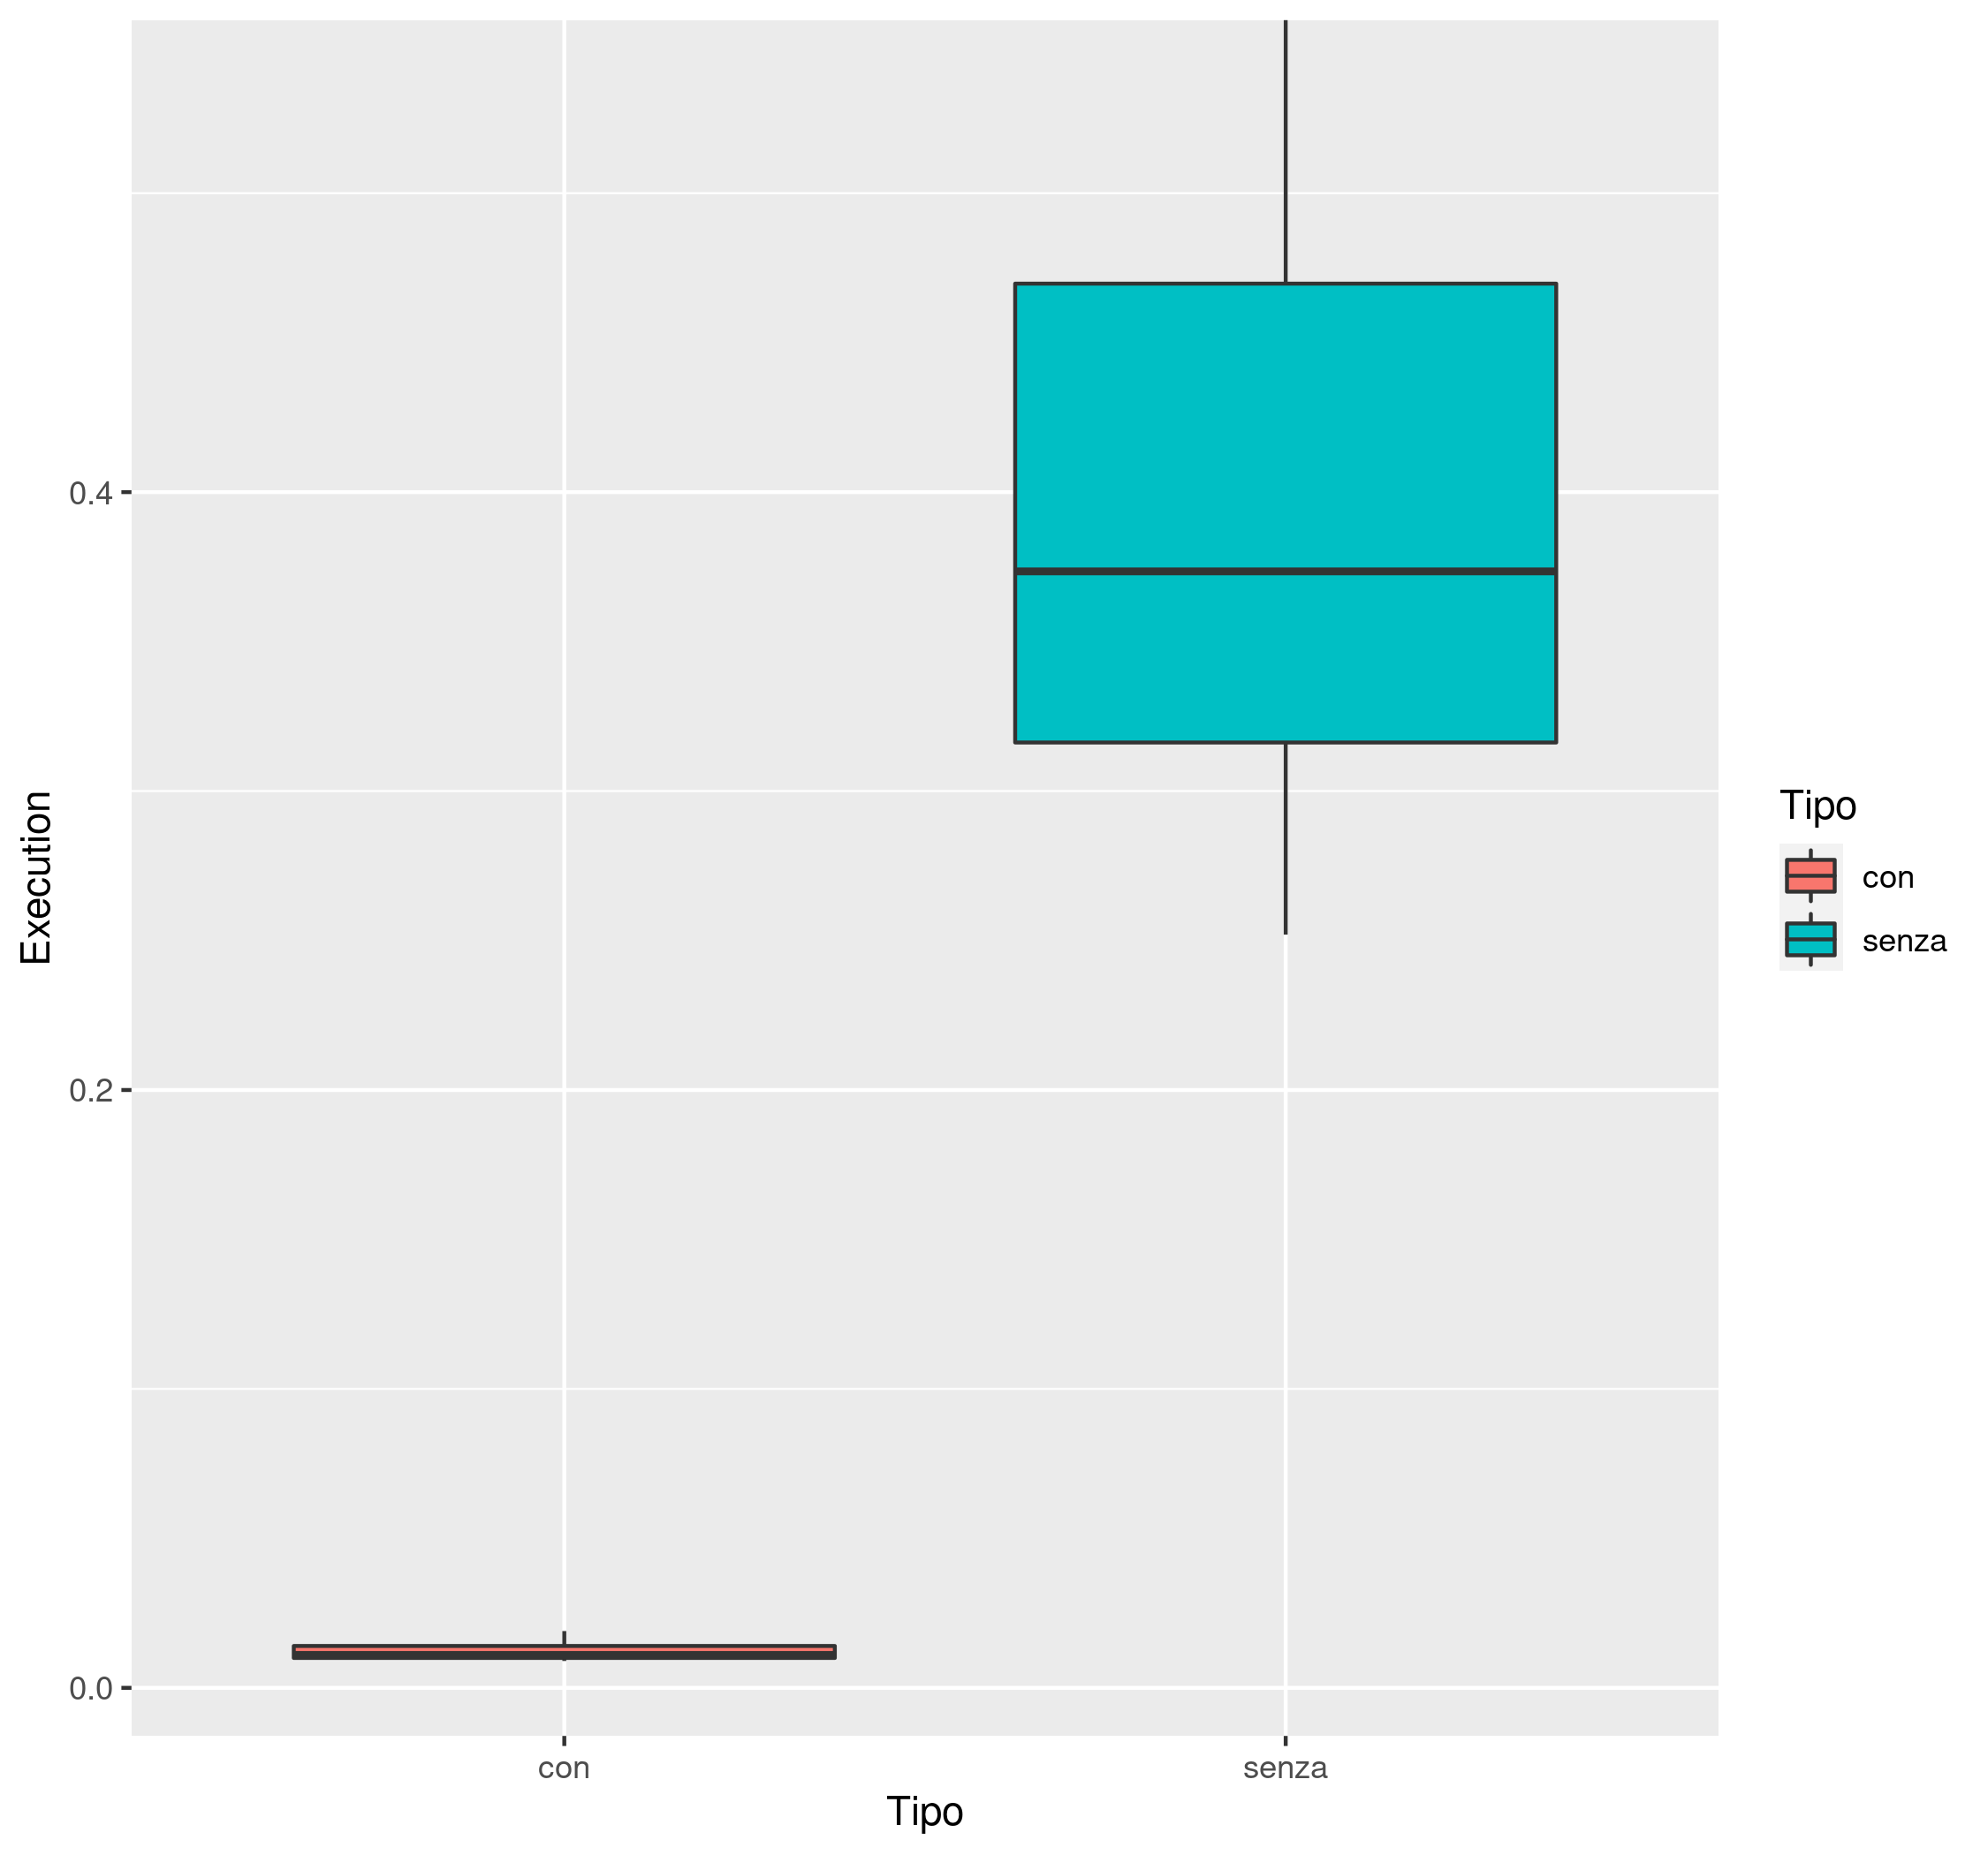
\includegraphics[width=0.5\textwidth]{execution_impiegato_dataAssunzione_selezione.png}
\newline
\newline
\textbf{Operazioni di modifica}
\newline
\newline
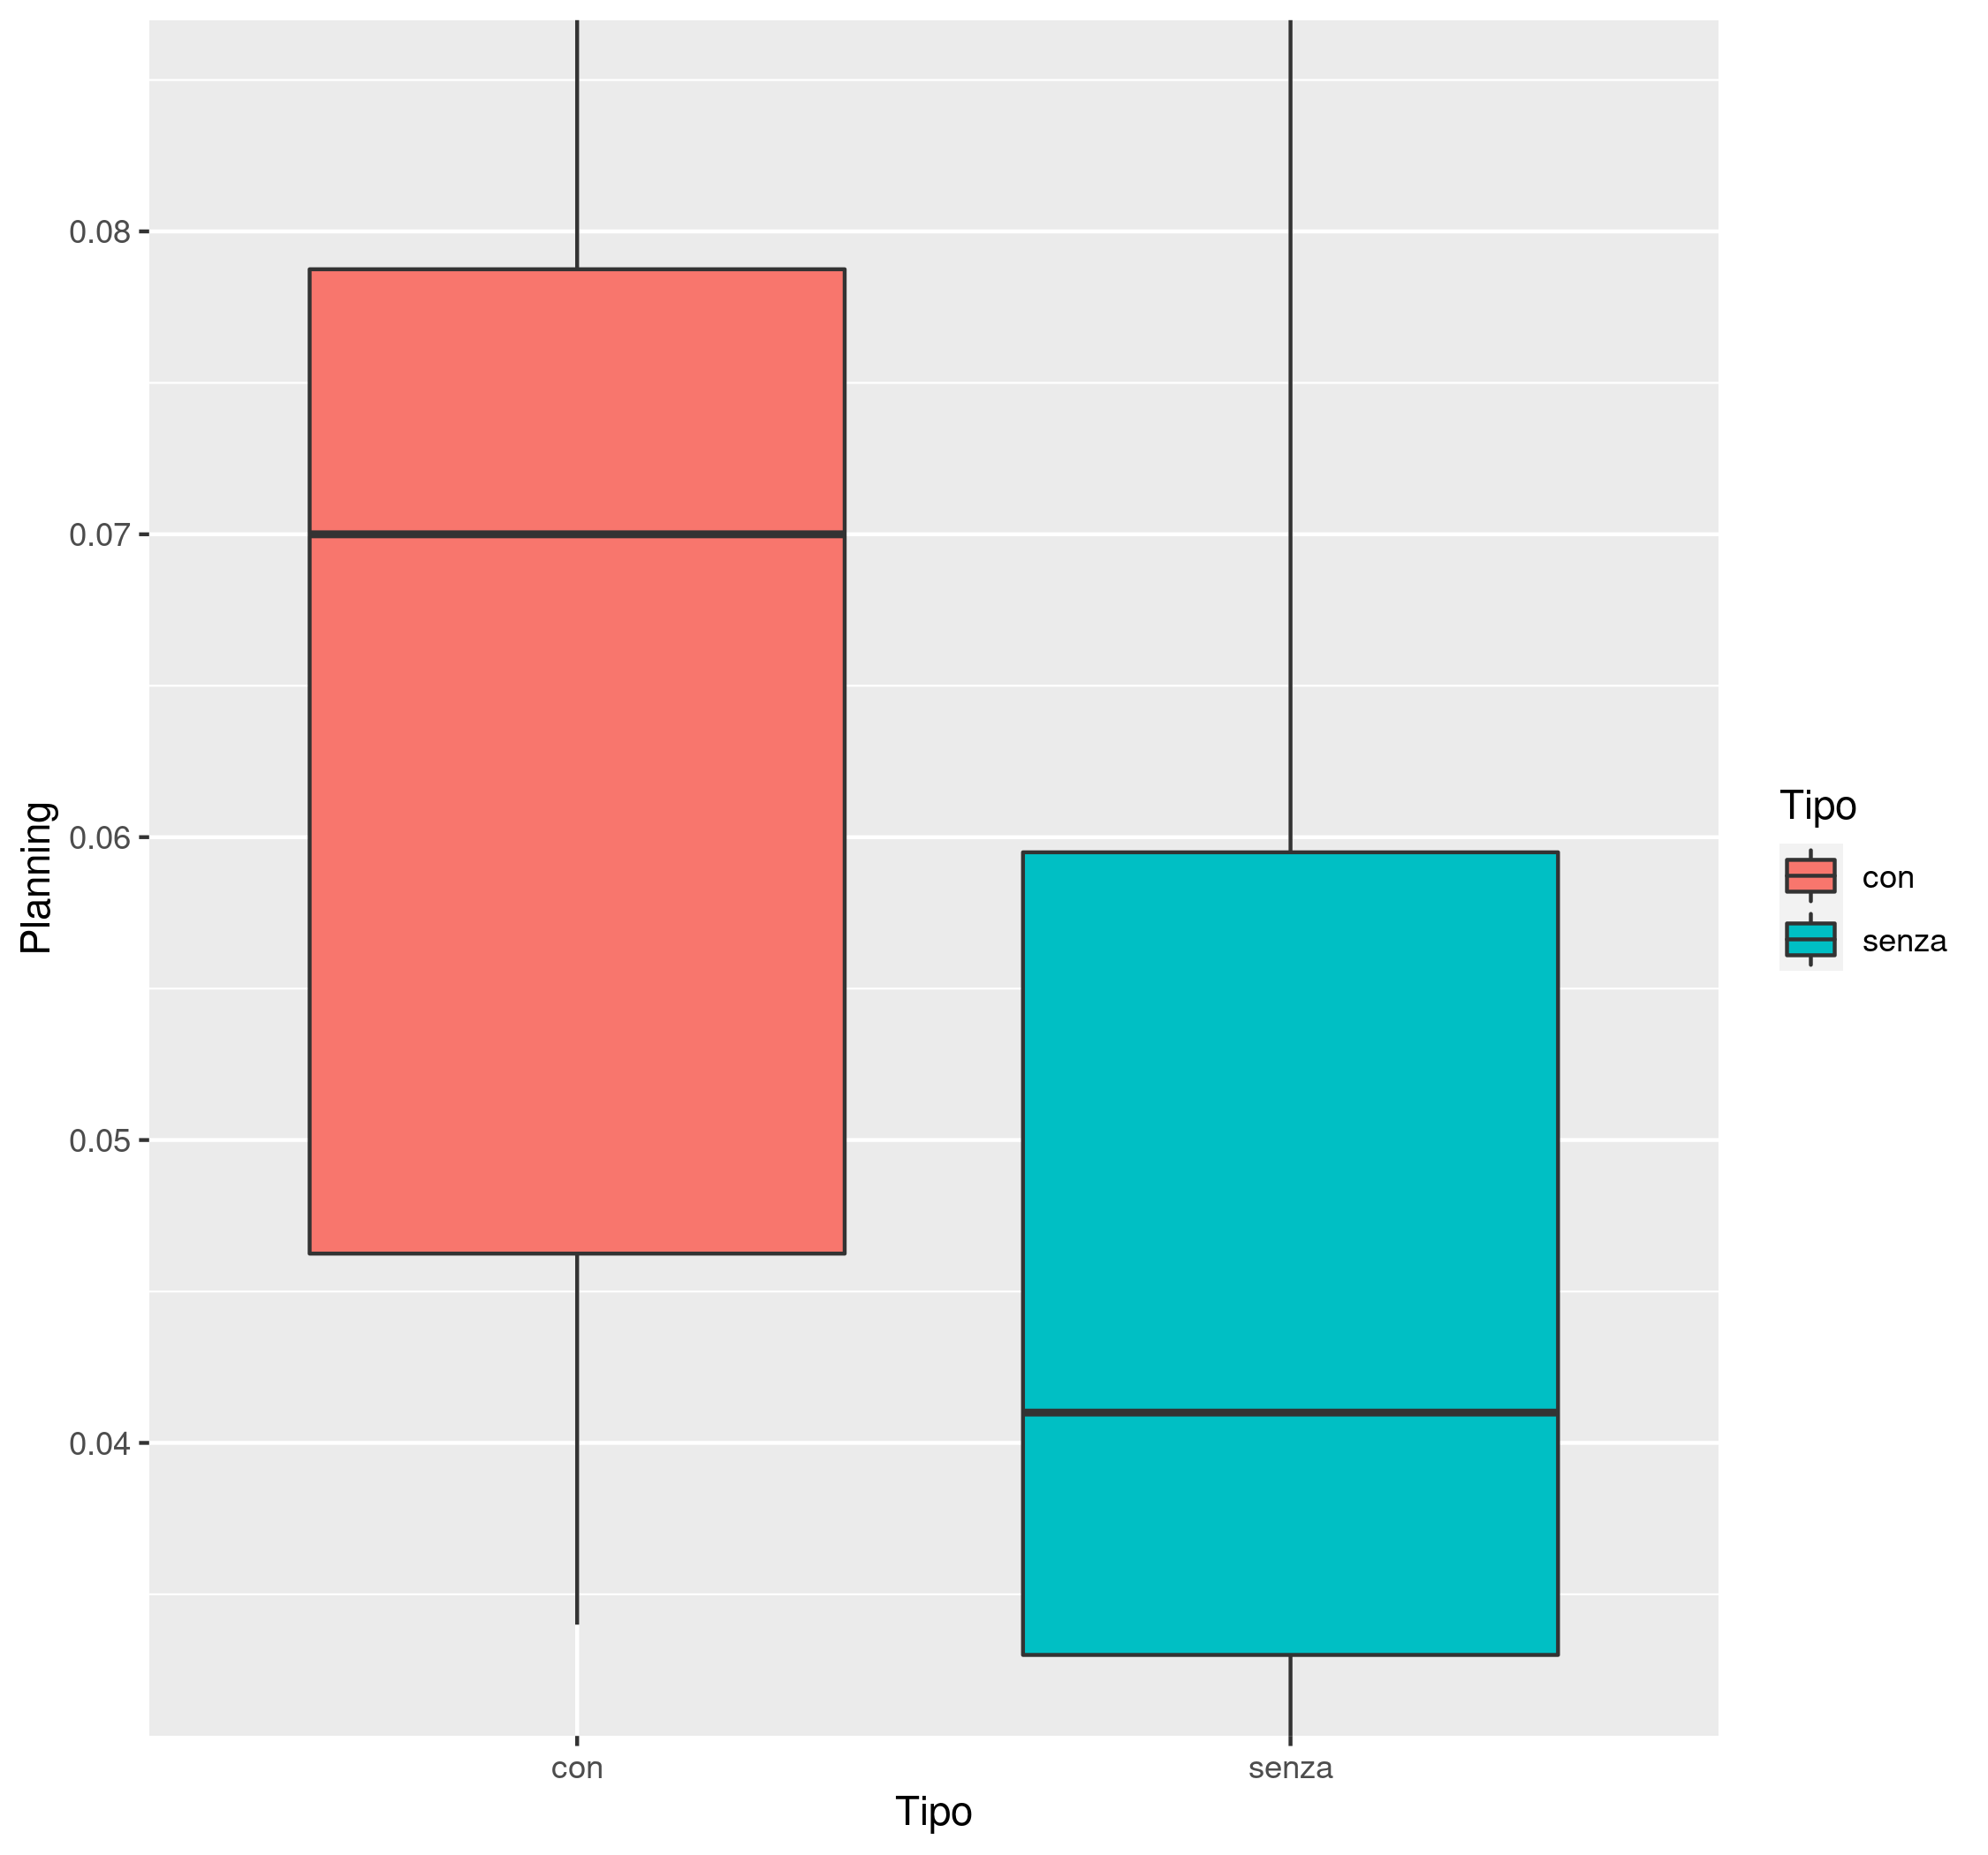
\includegraphics[width=0.5\textwidth]{planning_impiegato_dataAssunzione_modifica.png}
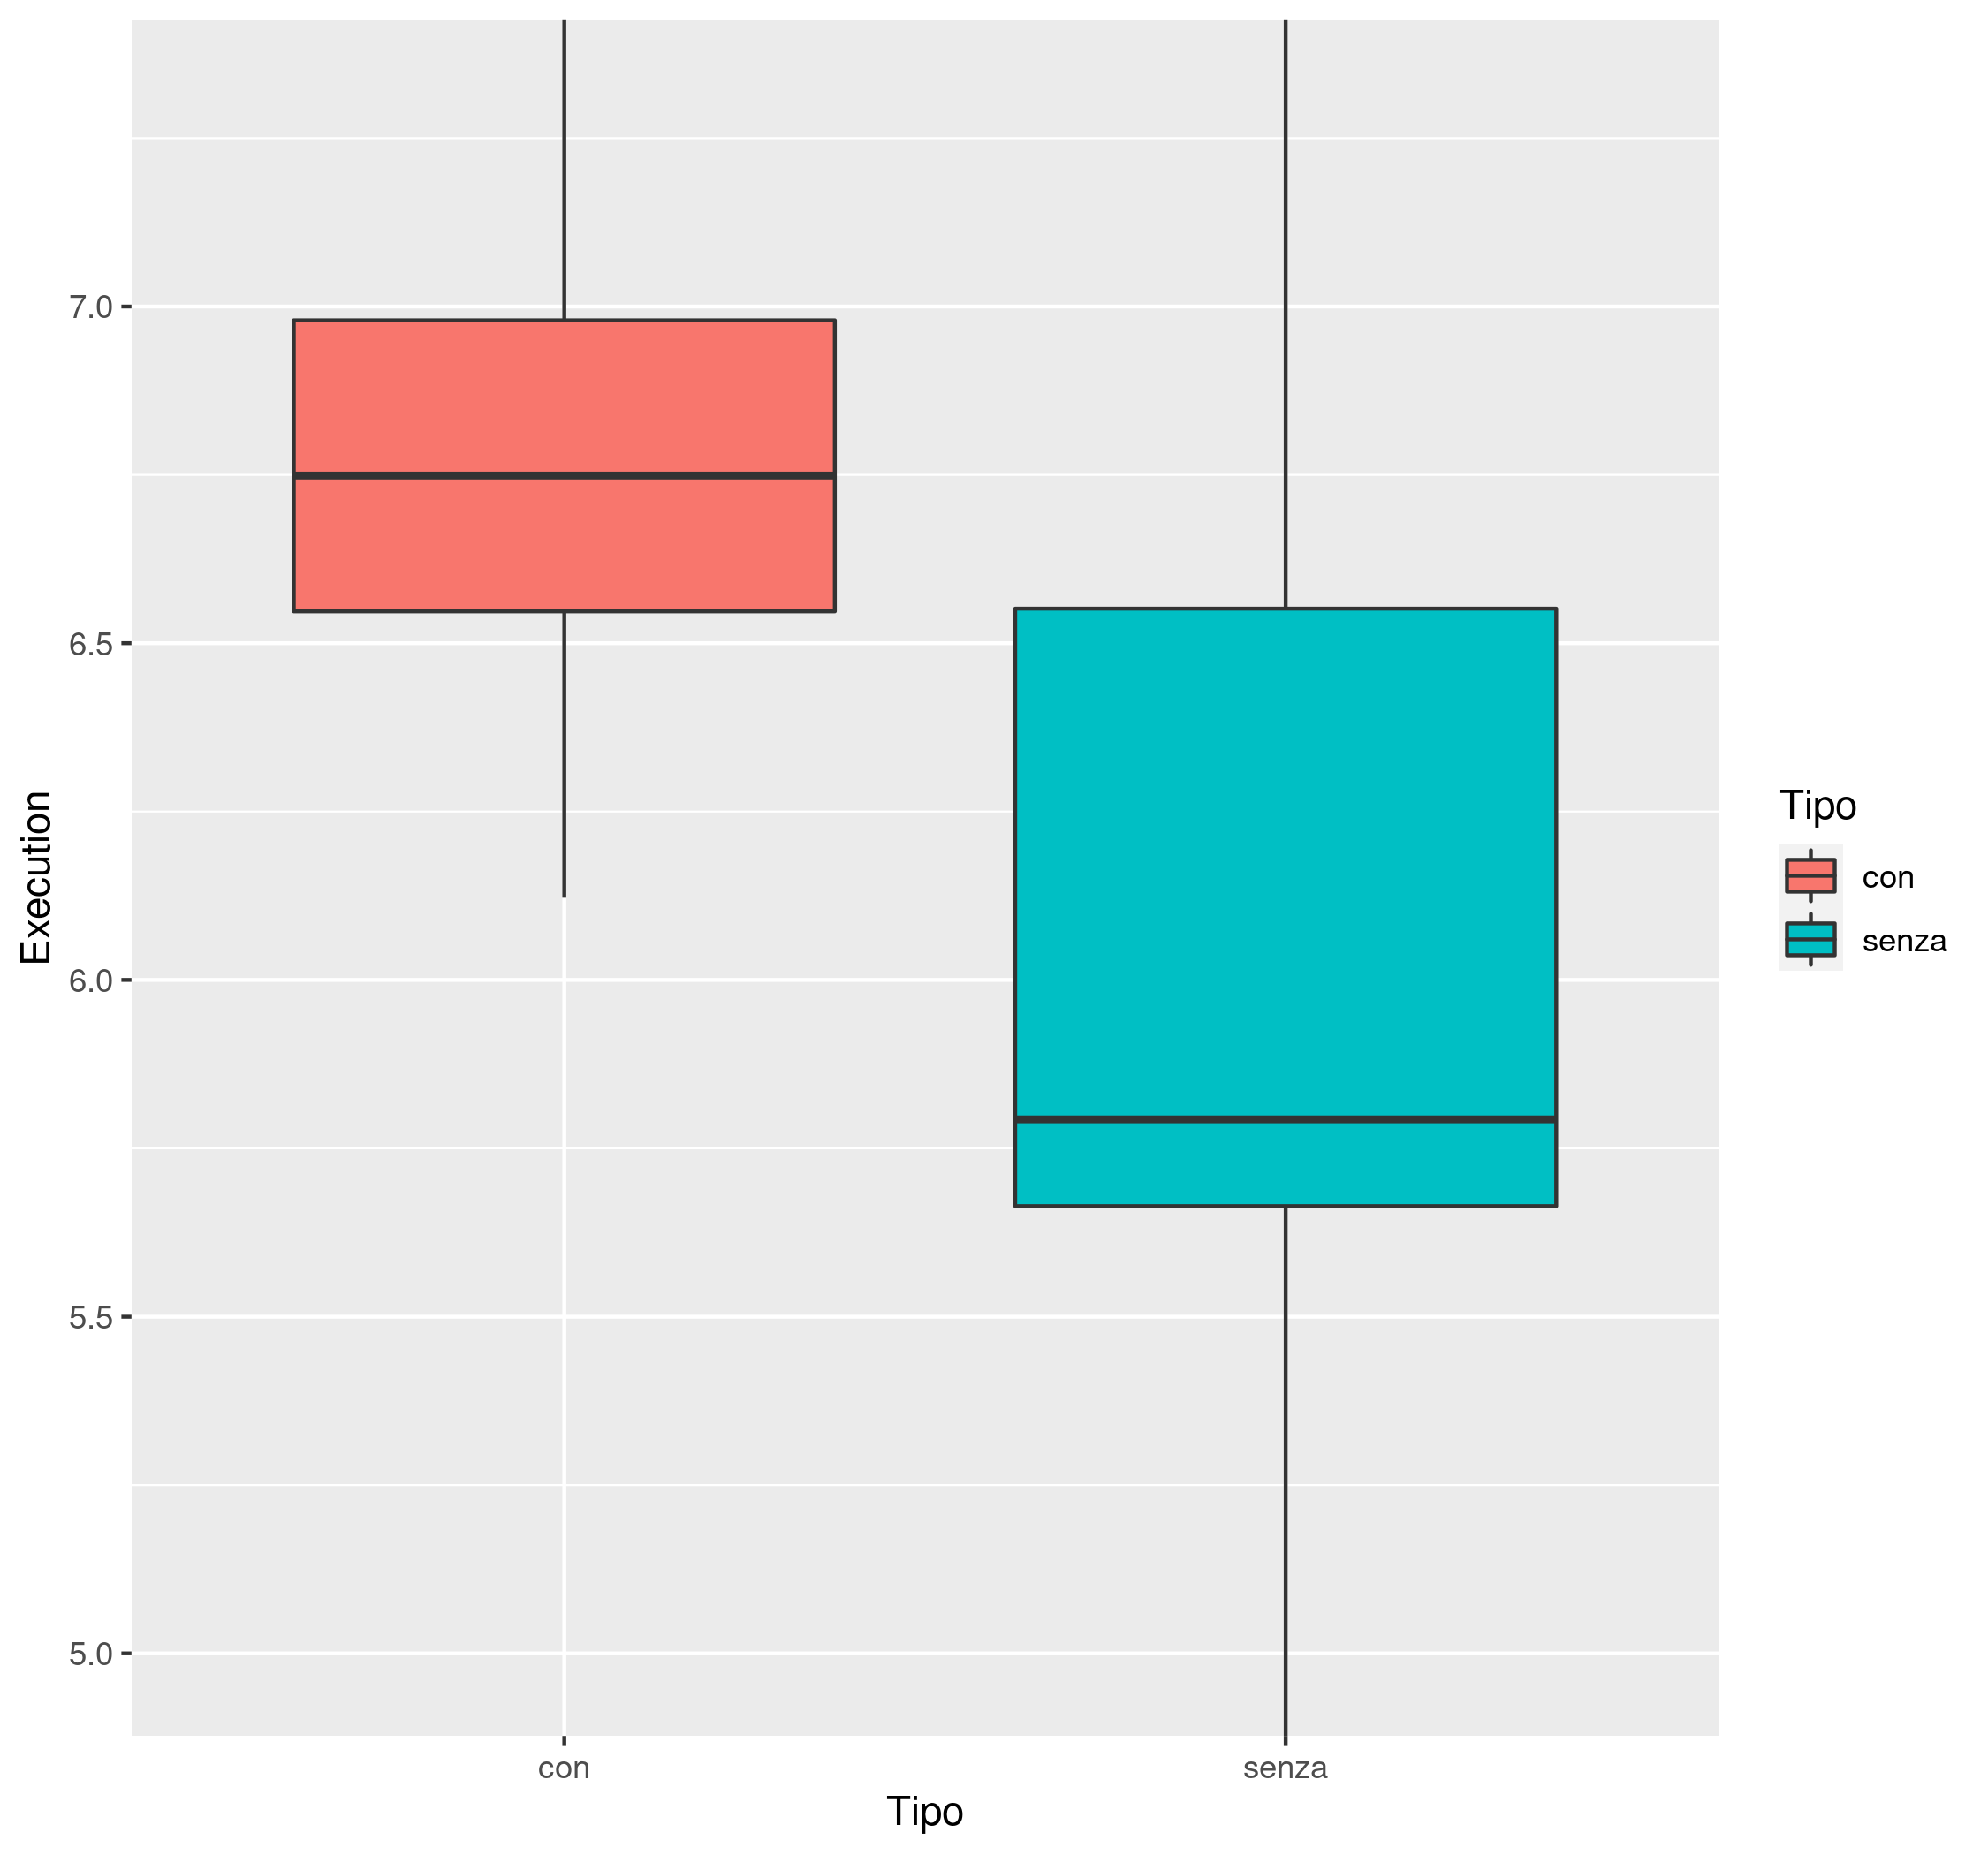
\includegraphics[width=0.5\textwidth]{execution_impiegato_dataAssunzione_modifica.png}
\newline
\newline
Visto l'esito del profiling e data la natura dell'attributo su cui si è costruito l'indice si ritiene di implementarlo.

\newpage

\subsubsection{Valutazione dell'indicizzazione di budget di progetto}
\textbf{Operazioni di selezione}
\begin{minted}{sql}
Interrogazione: explain analyse select * from progetto where budget>=100000
\end{minted}
\begin{table}[H]
\renewcommand{\arraystretch}{1.1}
\centering
\begin{tabular}{|p{4cm}|p{4cm}|p{0cm}|p{4cm}|p{4cm}|}
\cline{1-5}
Planning \textbf{senza} indice & Execution \textbf{senza} indice & & Planning \textbf{con} indice & Execution \textbf{con} indice \\ \cline{1-5}
0.048 & 0.042 & & 0.078 & 0.036 \\ \cline{1-5}
0.041 & 0.048 & & 0.037 & 0.03 \\ \cline{1-5}
0.024 & 0.041 & & 0.05 & 0.022 \\ \cline{1-5}
0.027 & 0.035 & & 0.041 & 0.022 \\ \cline{1-5}
0.019 & 0.033 & & 0.044 & 0.024 \\ \cline{1-5}
0.02 & 0.033 & & 0.059 & 0.046 \\ \cline{1-5}
0.019 & 0.023 & & 0.069 & 0.041 \\ \cline{1-5}
0.02 & 0.03 & & 0.041 & 0.022 \\ \cline{1-5}
0.019 & 0.031 & & 0.041 & 0.022 \\ \cline{1-5}
0.022 & 0.031 & & 0.032 & 0.029 \\ \cline{1-5}
0.037 & 0.041 & & 0.04 & 0.022 \\ \cline{1-5}
0.026 & 0.041 & & 0.046 & 0.026 \\ \cline{1-5}
0.027 & 0.023 & & 0.038 & 0.027 \\ \cline{1-5}
0.027 & 0.042 & & 0.031 & 0.031 \\ \cline{1-5}
0.072 & 0.052 & & 0.035 & 0.018 \\ \cline{1-5}
0.034 & 0.049 & & 0.089 & 0.051 \\ \cline{1-5}
0.04 & 0.042 & & 0.035 & 0.03 \\ \cline{1-5}
0.02 & 0.023 & & 0.045 & 0.033 \\ \cline{1-5}
0.027 & 0.023 & & 0.049 & 0.021 \\ \cline{1-5}
0.027 & 0.047 & & 0.043 & 0.029 \\ \cline{1-5}
0.034 & 0.04 & & 0.044 & 0.033 \\ \cline{1-5}
0.021 & 0.032 & & 0.027 & 0.02 \\ \cline{1-5}
0.02 & 0.031 & & 0.03 & 0.025 \\ \cline{1-5}
0.03 & 0.026 & & 0.034 & 0.018 \\ \cline{1-5}
0.02 & 0.025 & & 0.049 & 0.031 \\ \cline{1-5}
0.032 & 0.028 & & 0.056 & 0.031 \\ \cline{1-5}
0.027 & 0.032 & & 0.044 & 0.026 \\ \cline{1-5}
0.022 & 0.025 & & 0.041 & 0.023 \\ \cline{1-5}
0.027 & 0.037 & & 0.047 & 0.029 \\ \cline{1-5}
0.036 & 0.042 & & 0.061 & 0.045 \\ \cline{1-5}
\end{tabular}
\end{table}

\newpage
\noindent
\textbf{Operazioni di modifica}
\begin{minted}{sql}
Interrogazione: explain analyse update progetto set budget=budget*0.75 where citta='Atlanta'
\end{minted}
\begin{table}[H]
\renewcommand{\arraystretch}{1.2}
\centering
\begin{tabular}{|p{4cm}|p{4cm}|p{0cm}|p{4cm}|p{4cm}|}
\cline{1-5}
Planning \textbf{senza} indice & Execution \textbf{senza} indice & & Planning \textbf{con} indice & Execution \textbf{con} indice \\ \cline{1-5}
0.065 & 0.101 & & 0.055 & 0.088 \\ \cline{1-5}
0.063 & 0.08 & & 0.035 & 0.07 \\ \cline{1-5}
0.046 & 0.079 & & 0.029 & 0.062 \\ \cline{1-5}
0.034 & 0.072 & & 0.027 & 0.061 \\ \cline{1-5}
0.04 & 0.07 & & 0.035 & 0.062 \\ \cline{1-5}
0.036 & 0.064 & & 0.034 & 0.06 \\ \cline{1-5}
0.038 & 0.064 & & 0.027 & 0.06 \\ \cline{1-5}
0.041 & 0.071 & & 0.035 & 0.063 \\ \cline{1-5}
0.045 & 0.085 & & 0.033 & 0.061 \\ \cline{1-5}
0.039 & 0.075 & & 0.033 & 0.061 \\ \cline{1-5}
0.043 & 0.091 & & 0.034 & 0.061 \\ \cline{1-5}
0.034 & 0.084 & & 0.033 & 0.06 \\ \cline{1-5}
0.03 & 0.076 & & 0.035 & 0.062 \\ \cline{1-5}
0.035 & 0.096 & & 0.051 & 0.074 \\ \cline{1-5}
0.026 & 0.057 & & 0.051 & 0.125 \\ \cline{1-5}
0.039 & 0.054 & & 0.046 & 0.077 \\ \cline{1-5}
0.025 & 0.058 & & 0.057 & 0.112 \\ \cline{1-5}
0.024 & 0.054 & & 0.037 & 0.075 \\ \cline{1-5}
0.03 & 0.049 & & 0.037 & 0.067 \\ \cline{1-5}
0.03 & 0.053 & & 0.039 & 0.072 \\ \cline{1-5}
0.024 & 0.054 & & 0.042 & 0.073 \\ \cline{1-5}
0.026 & 0.056 & & 0.103 & 0.072 \\ \cline{1-5}
0.056 & 0.093 & & 0.056 & 0.095 \\ \cline{1-5}
0.038 & 0.074 & & 0.078 & 0.136 \\ \cline{1-5}
0.04 & 0.066 & & 0.052 & 0.125 \\ \cline{1-5}
0.056 & 0.093 & & 0.035 & 0.062 \\ \cline{1-5}
0.042 & 0.075 & & 0.035 & 0.061 \\ \cline{1-5}
0.047 & 0.091 & & 0.026 & 0.064 \\ \cline{1-5}
0.073 & 0.13 & & 0.035 & 0.064 \\ \cline{1-5}
0.05 & 0.112 & & 0.034 & 0.101 \\ \cline{1-5}
\end{tabular}
\end{table}
\noindent
\newline
\textbf{Considerazioni sullo spazio occupato}
\newline
\newline
Sfruttando le seguenti interrogazioni è possibile conoscere lo spazio occupato dalla tabella e dagli indici:
\begin{minted}{sql}
SELECT pg_size_pretty(pg_total_relation_size ('progetto'));
SELECT pg_size_pretty(pg_indexes_size ('progetto'));
\end{minted}
Per impiegato il risultato è di \textbf{72kB} prima dell'indicizzazione e \textbf{88kB} a seguito di essa con una dimensione dell'indice di \textbf{16kB}.

\newpage
\noindent
\newline
Concludiamo visualizzando i risultati della profilazione tramite box plot
\newline
\newline
\textbf{Operazioni di selezione}
\newline
\newline
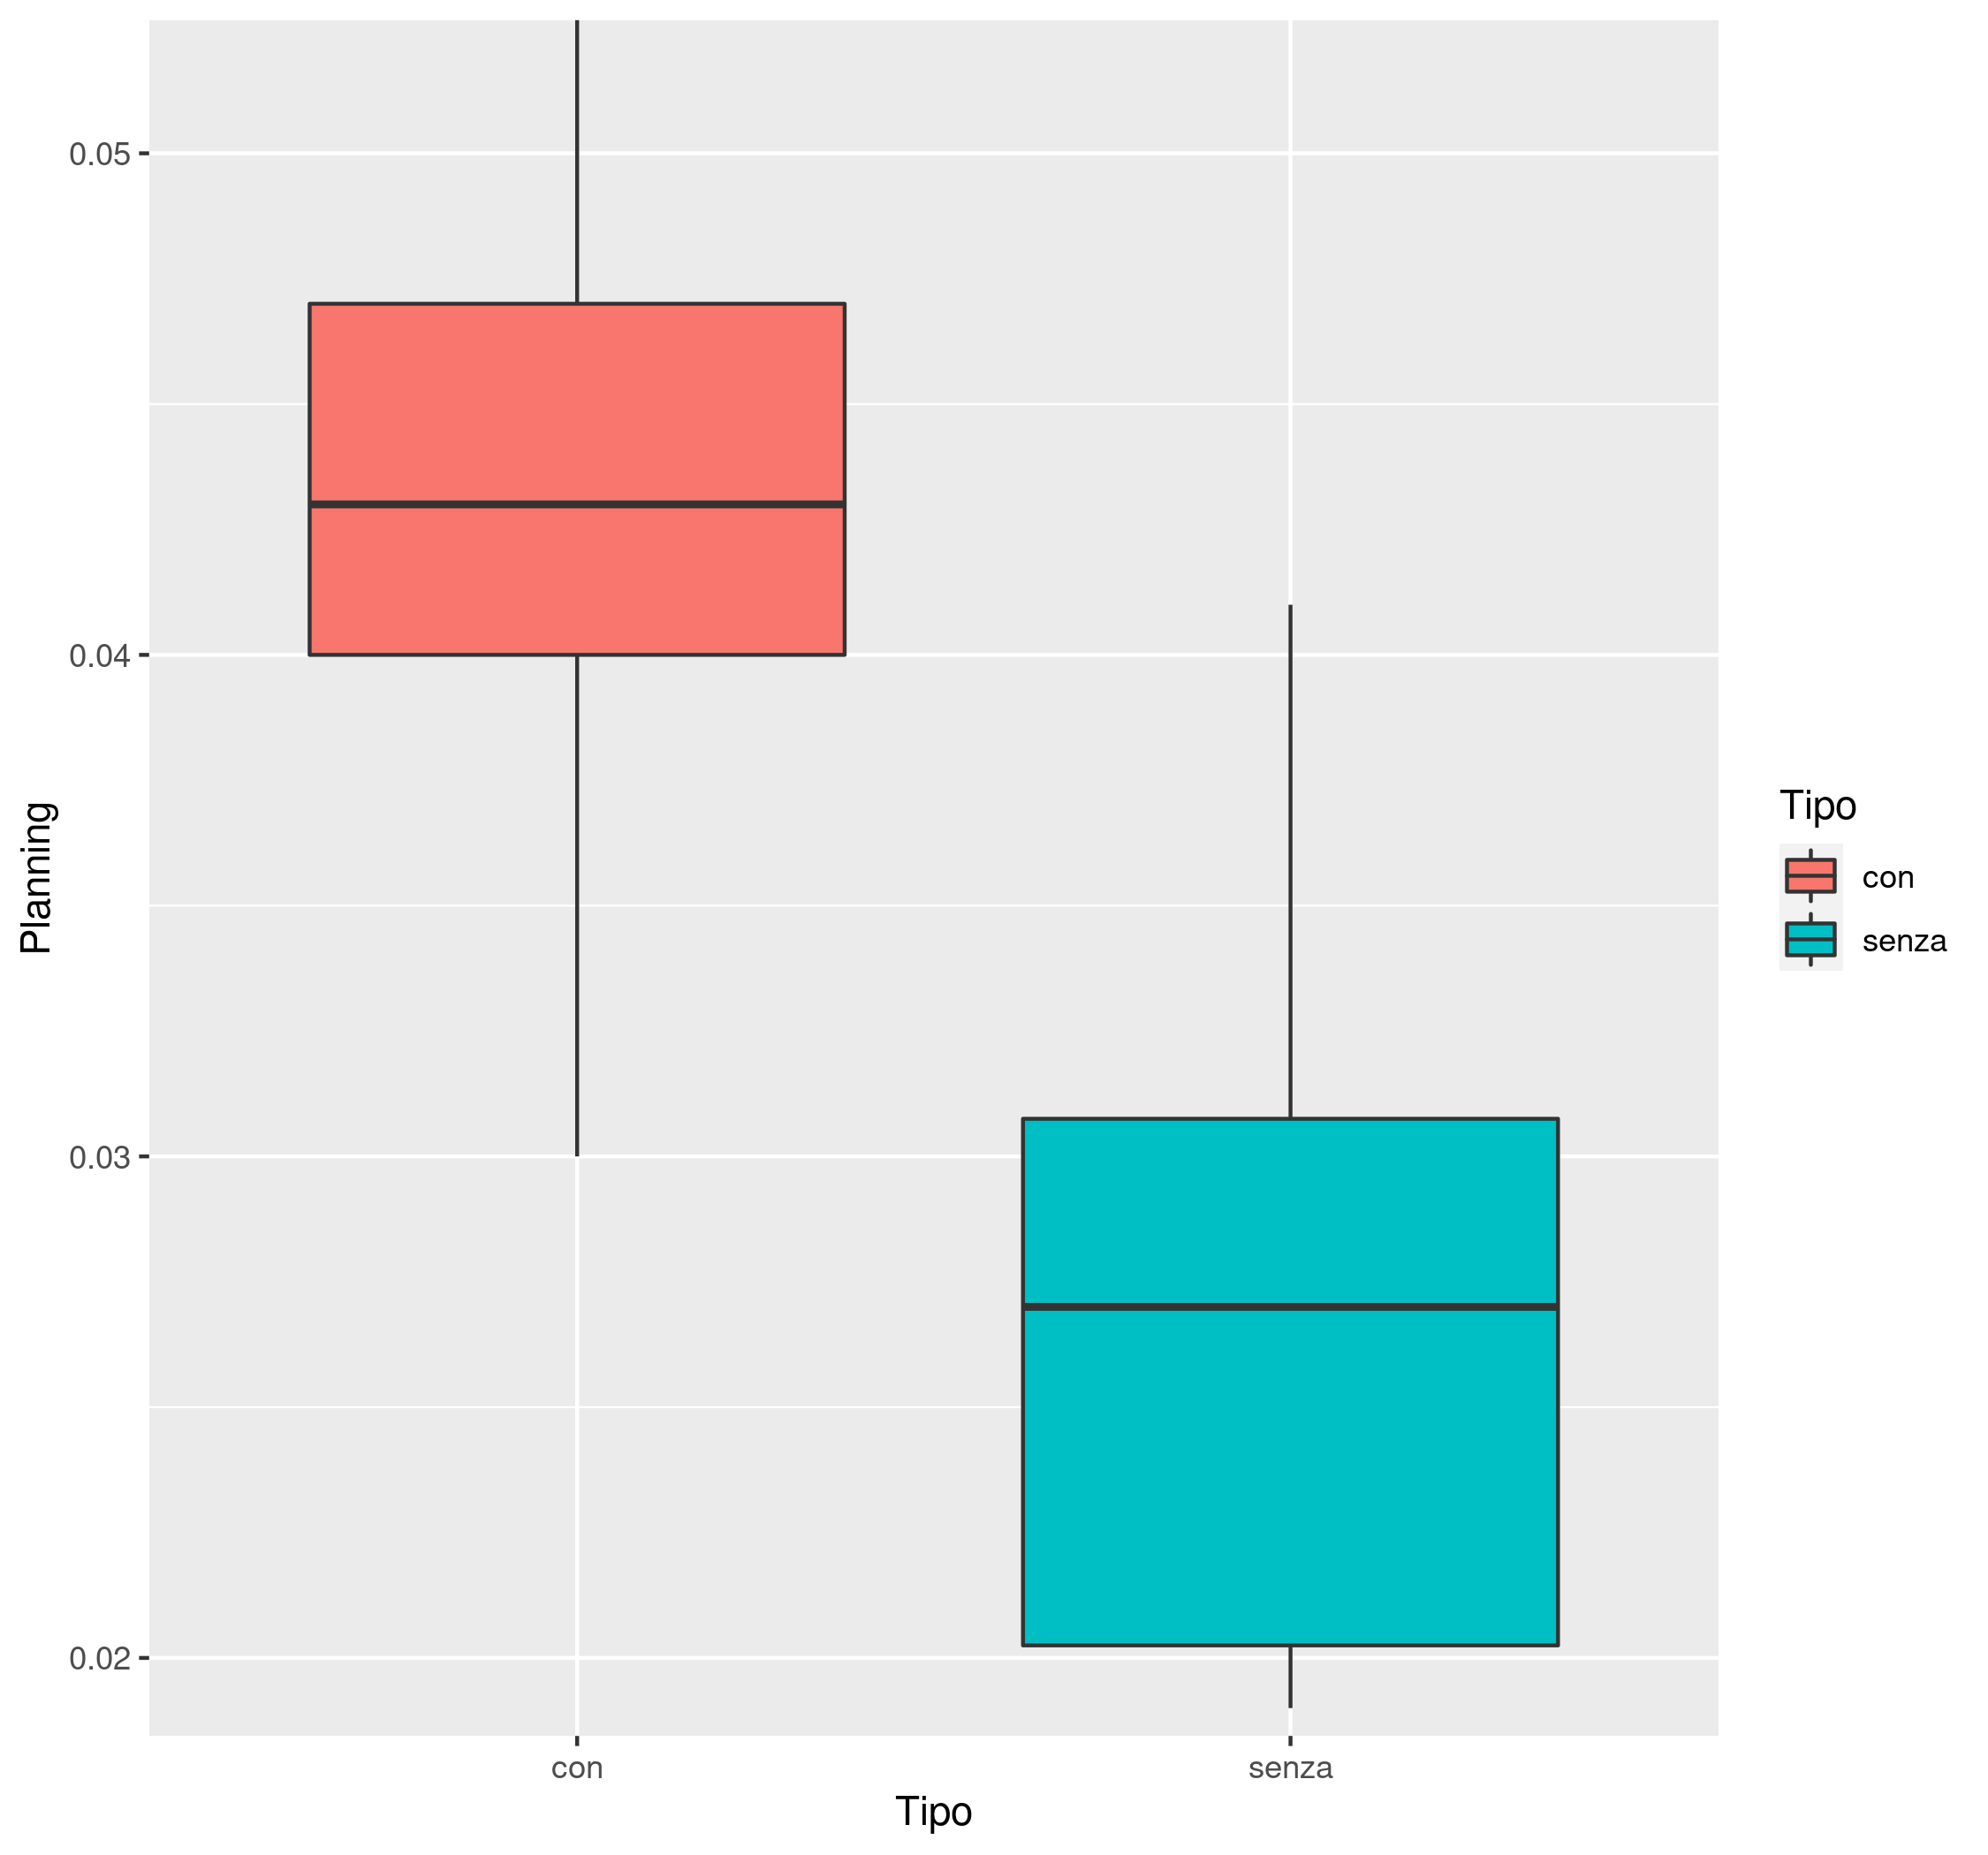
\includegraphics[width=0.5\textwidth]{planning_progetto_budget_selezione.png}
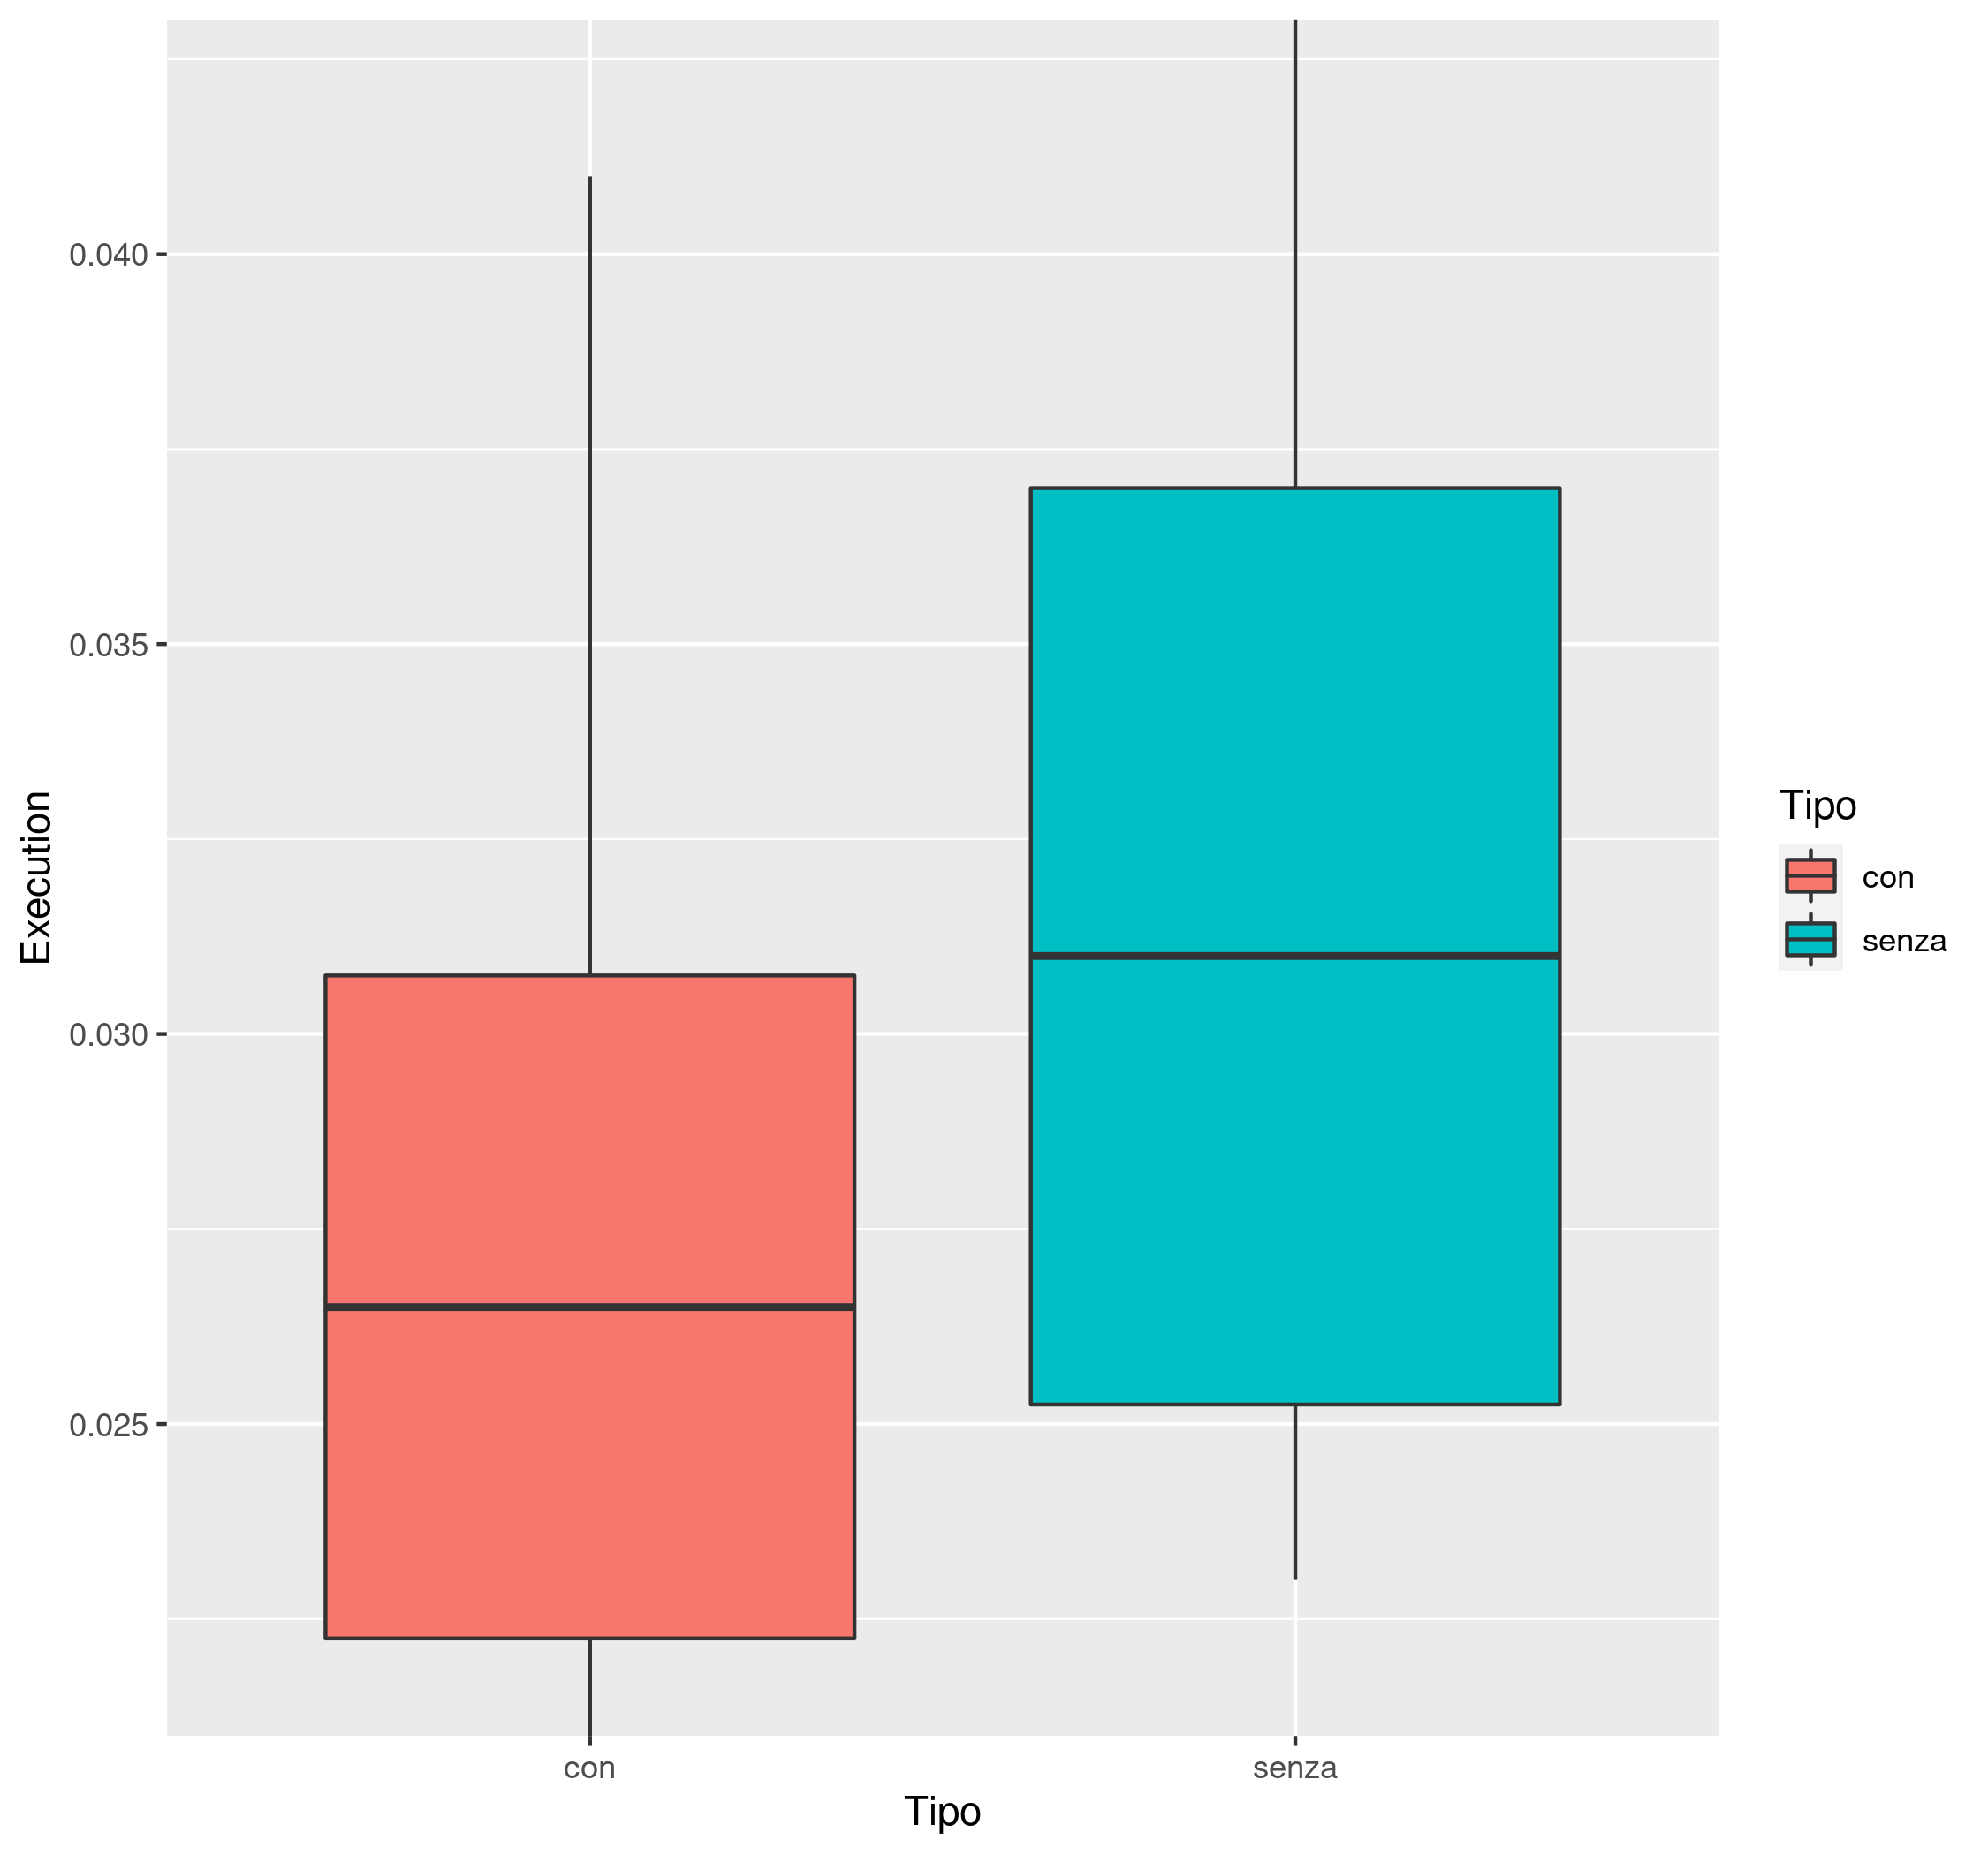
\includegraphics[width=0.5\textwidth]{execution_progetto_budget_selezione.png}
\newline
\newline
\textbf{Operazioni di modifica}
\newline
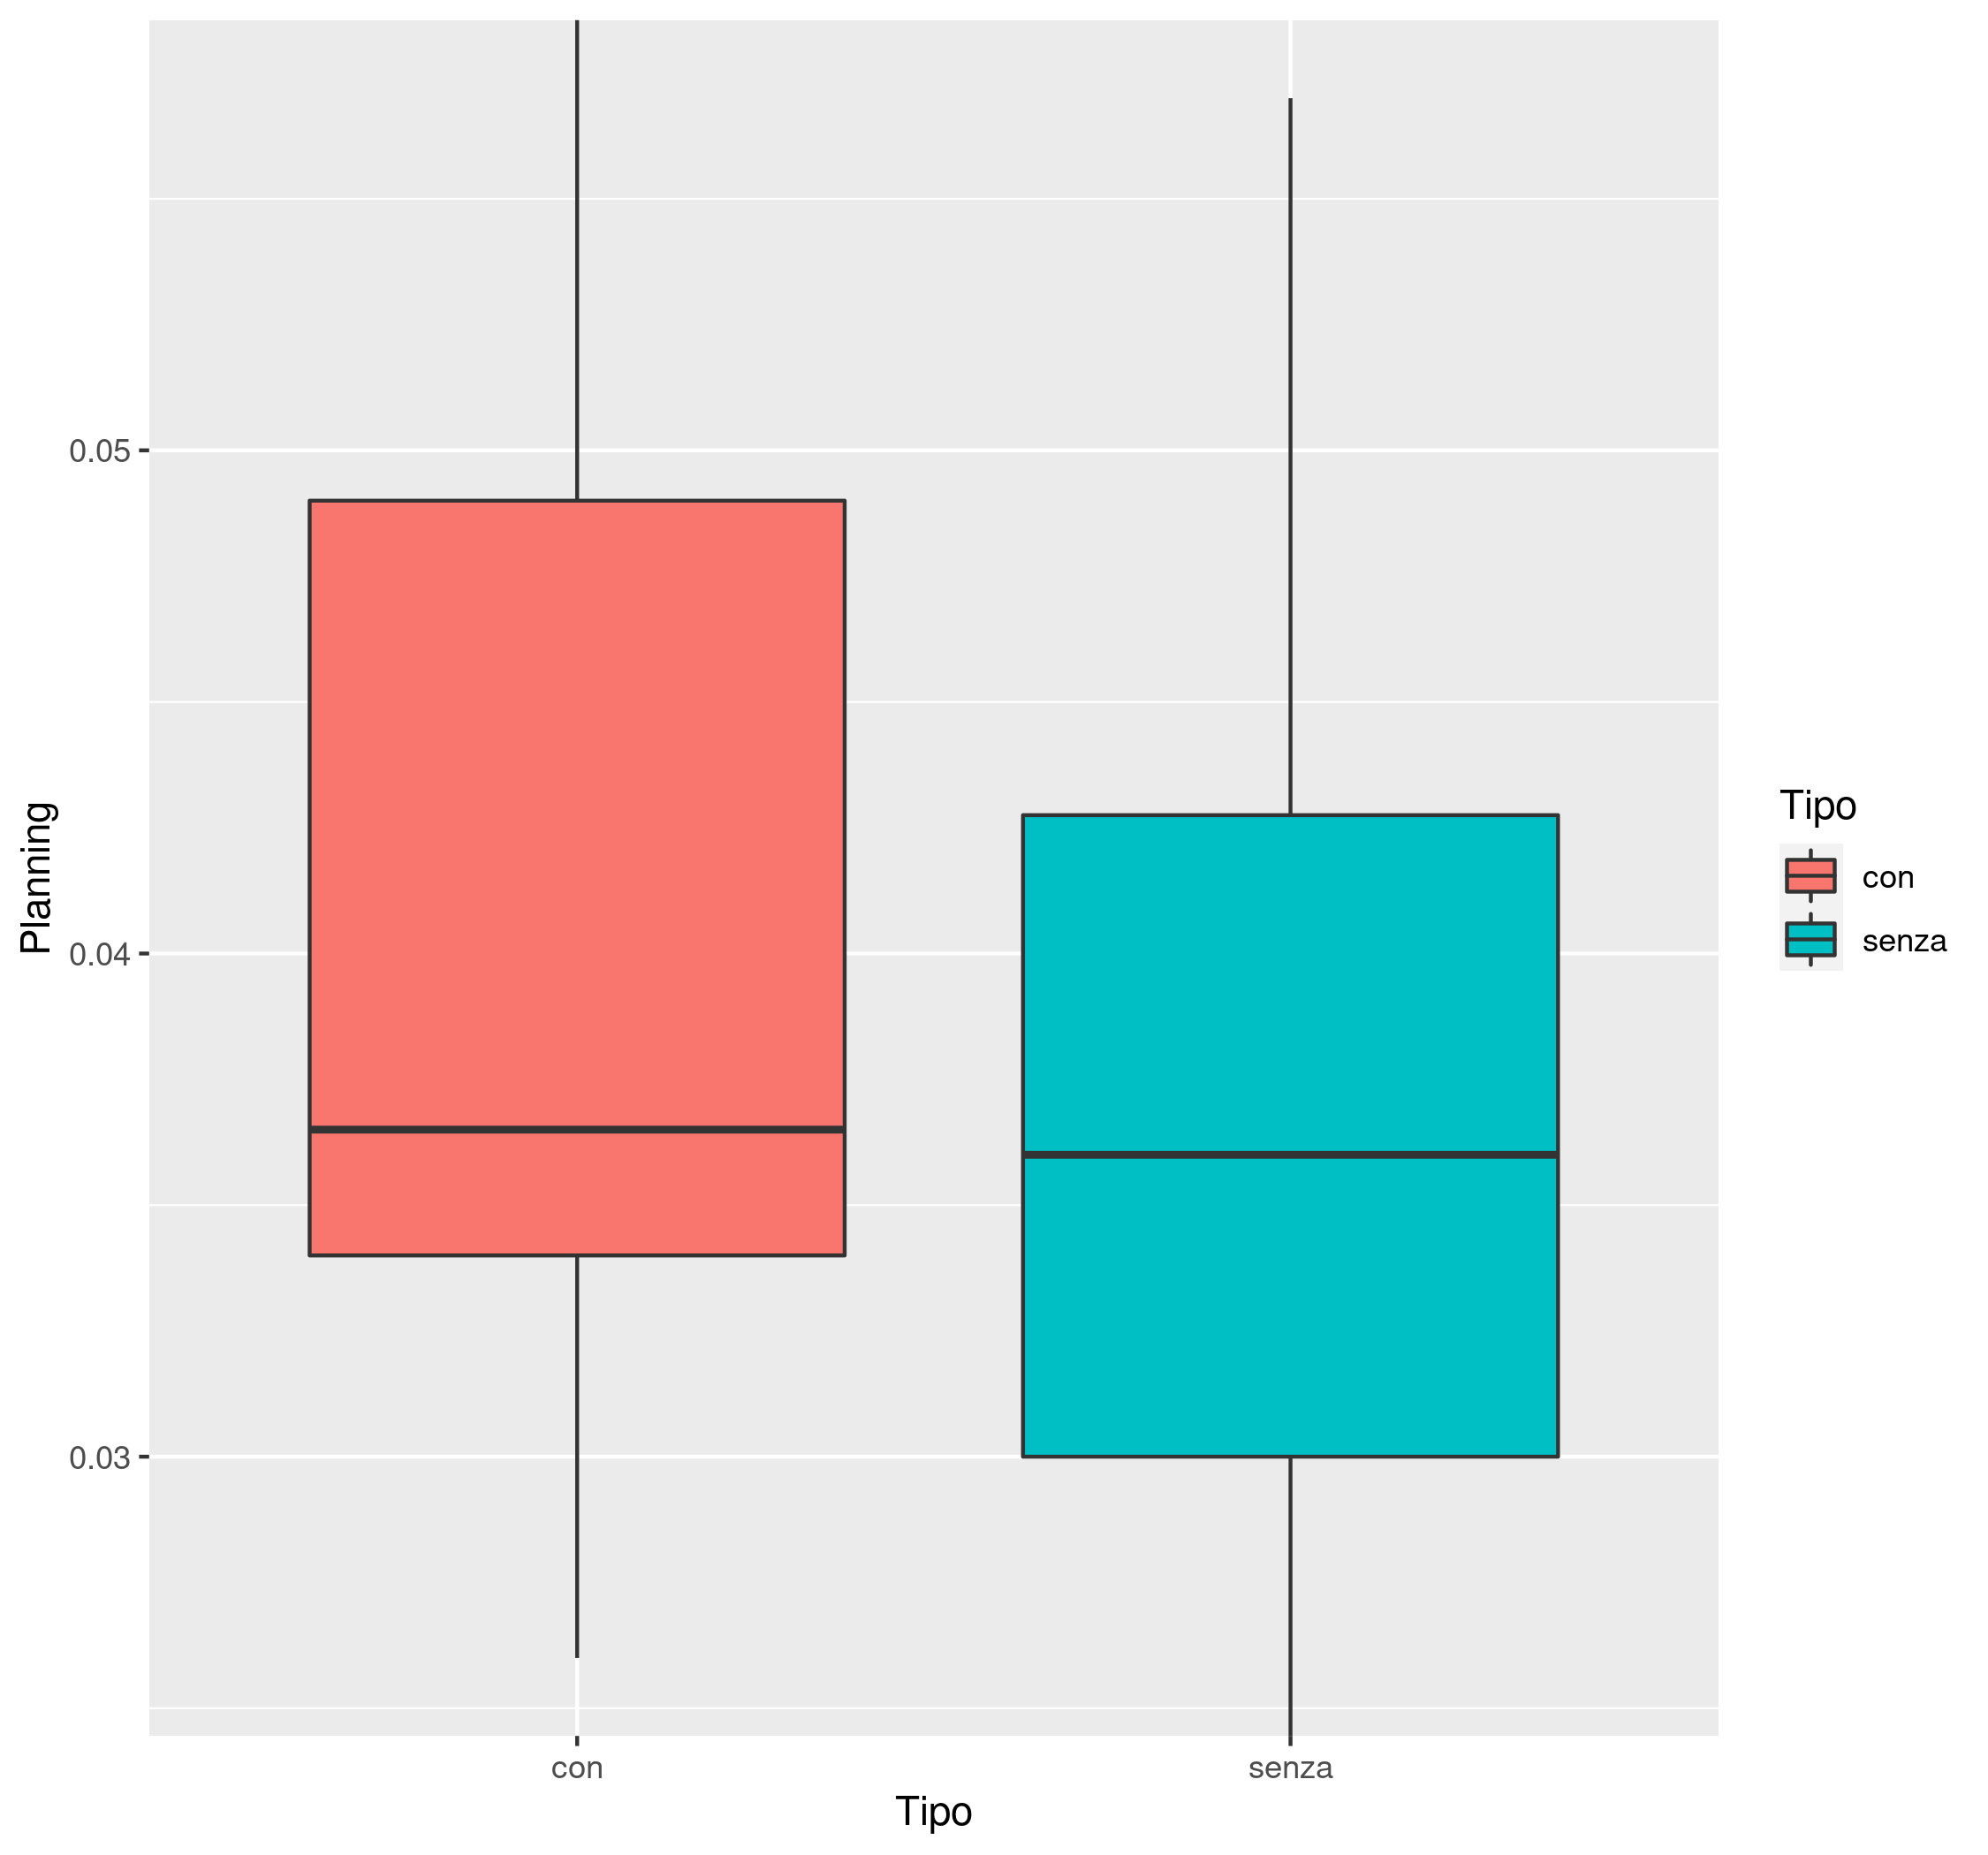
\includegraphics[width=0.5\textwidth]{planning_progetto_budget_modifica.png}
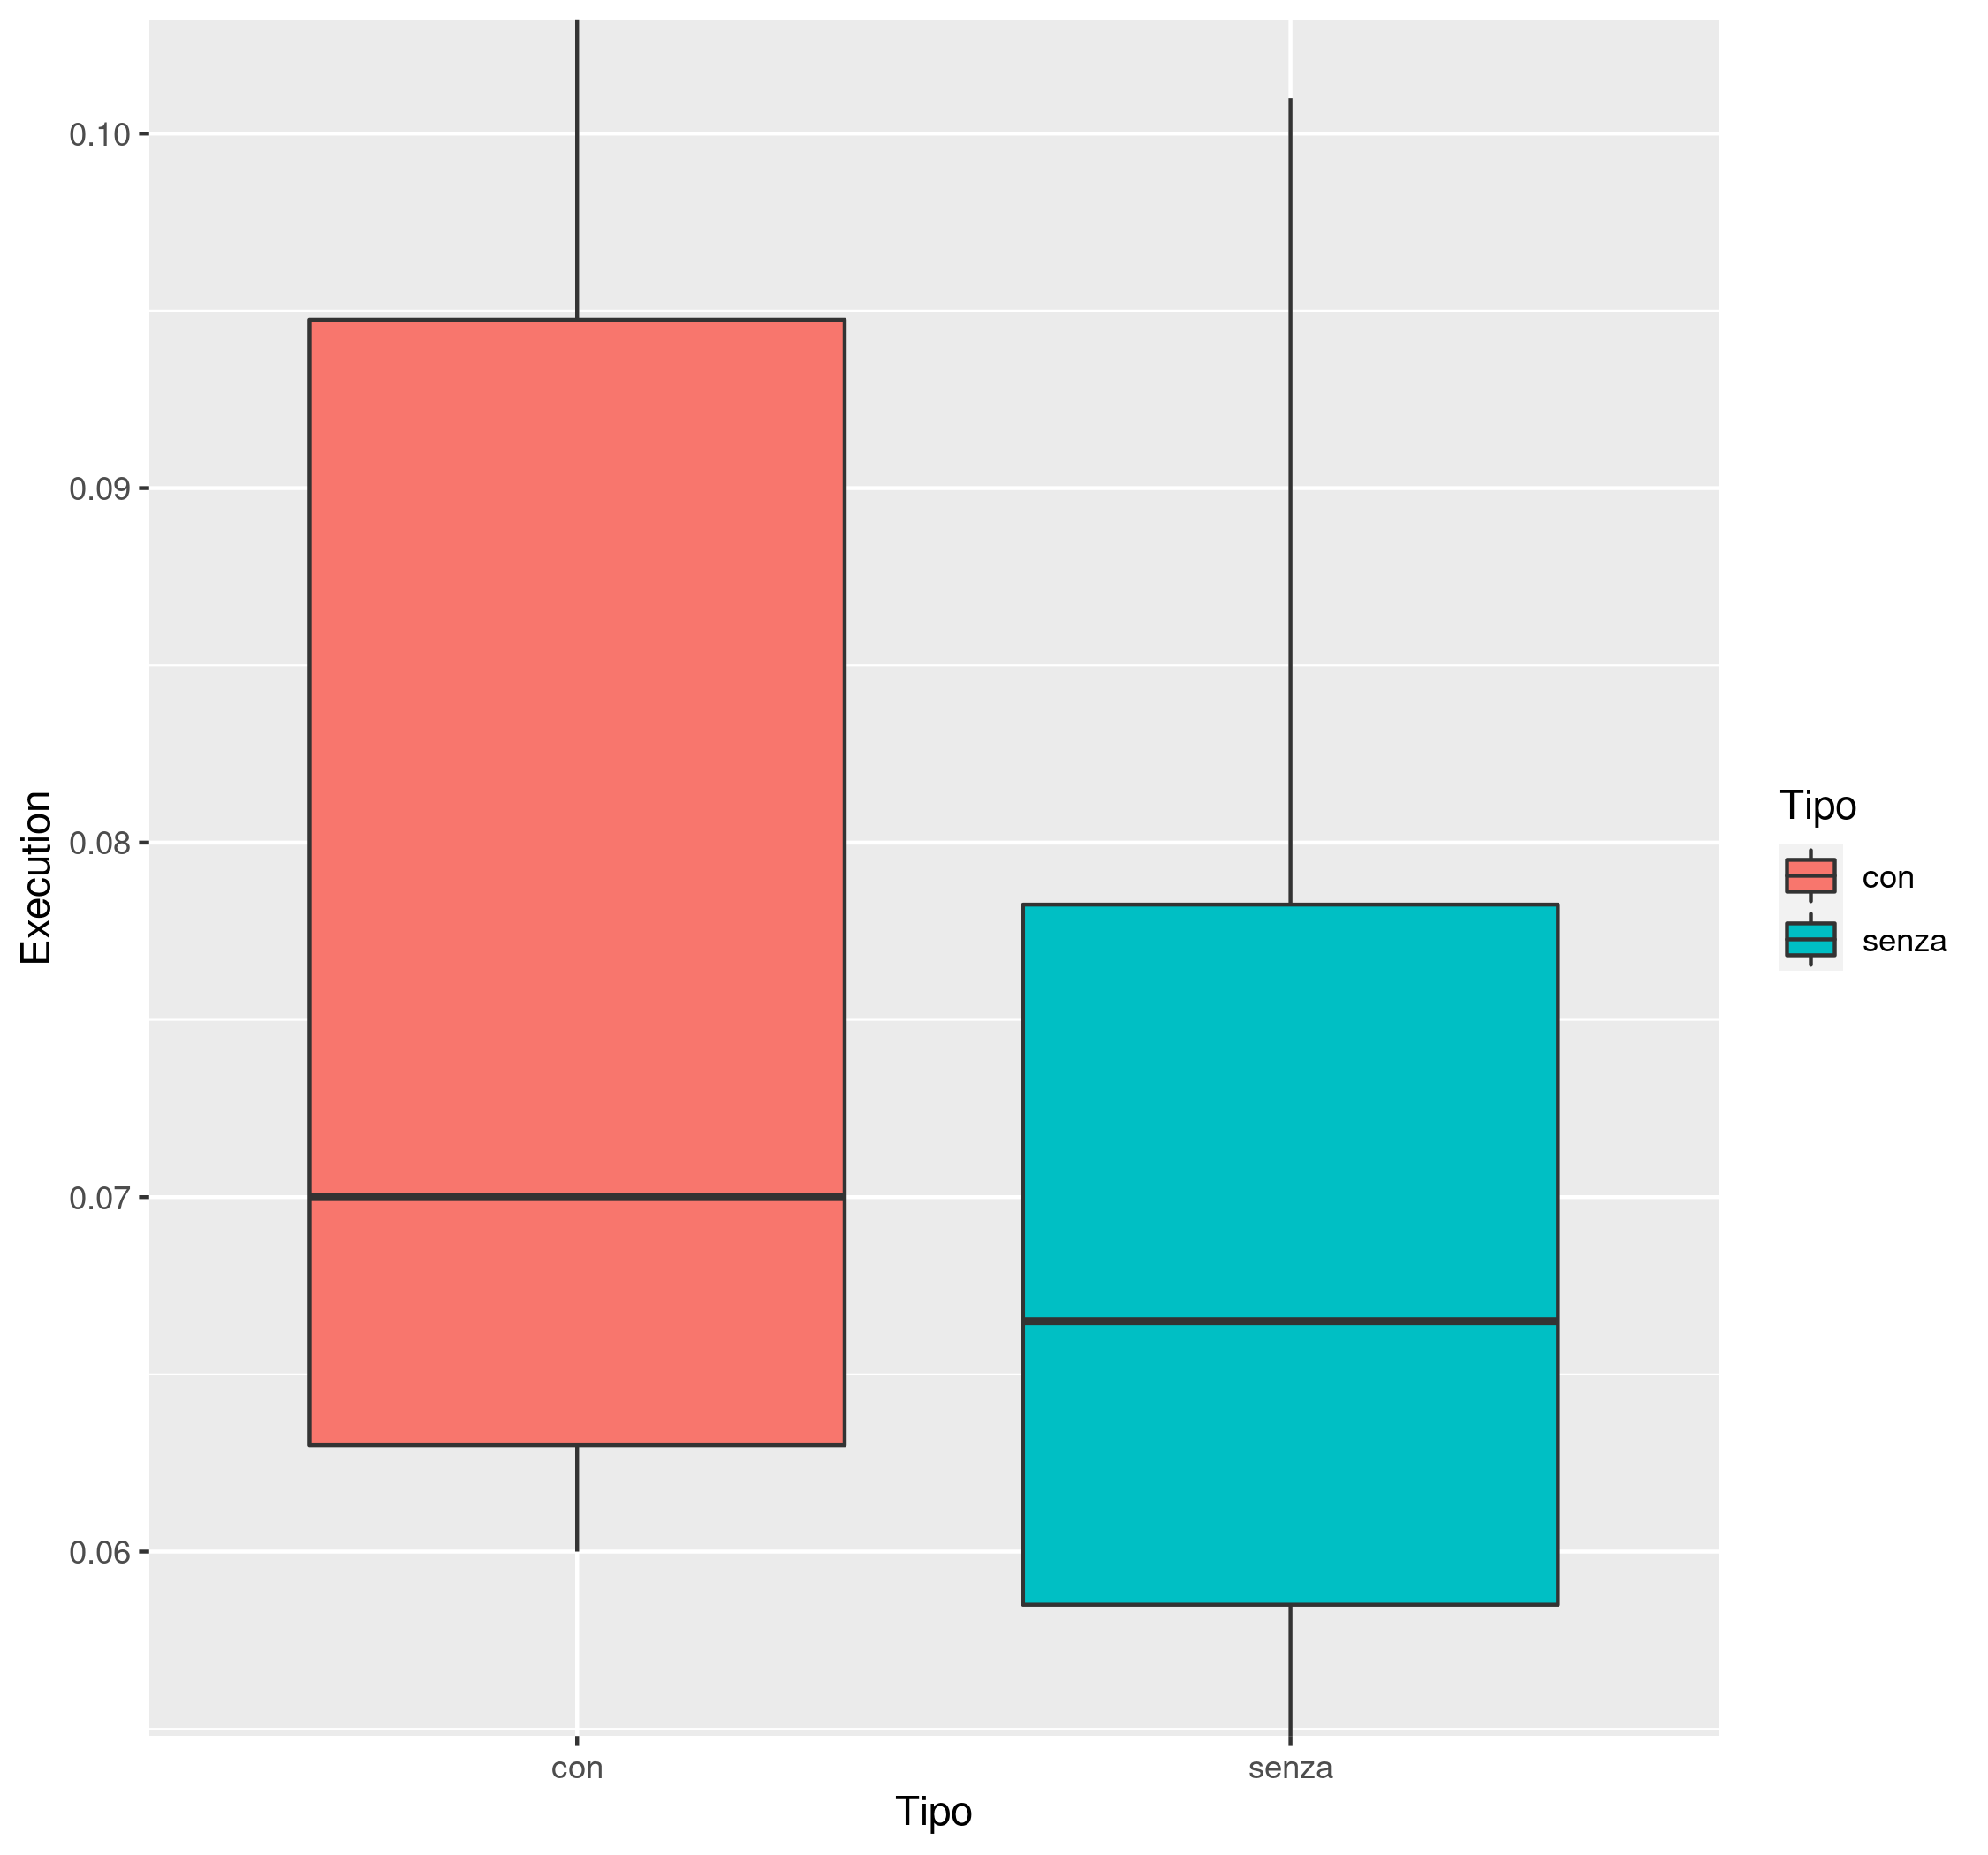
\includegraphics[width=0.5\textwidth]{execution_progetto_budget_modifica.png}
\newline
\newline
Visto l'esito del profiling e data la natura dell'attributo su cui si è costruito l'indice si ritiene di implementarlo.
 
\newpage

\section{Implementazione}

\subsection{Definizione delle tabelle}
Seguono le tabelle definite sulla base dello \hyperlink{page.15}{schema relazionale}.
\begin{minted}{sql}
CREATE TABLE fornitore (
  partitaiva numeric(11, 0) PRIMARY KEY, 
  nome varchar(50), 
  via varchar(50), 
  civico integer, 
  citta varchar(30)
);

CREATE TABLE dipartimento (
  nome varchar(50) PRIMARY KEY, 
  recapito_telefonico numeric(10, 0) UNIQUE, 
  numero_fornitori integer NOT null DEFAULT 0
);

CREATE TABLE rifornisce (
  dipartimento varchar(50) REFERENCES dipartimento(nome), 
  fornitore numeric(11, 0) REFERENCES fornitore(partitaiva), 
  PRIMARY KEY (dipartimento, fornitore)
);

CREATE TABLE lingua (
  lingua varchar(20) PRIMARY KEY
);

CREATE TABLE impiegato (
  matricola integer PRIMARY KEY, 
  nome varchar (20), 
  cognome varchar (20), 
  data_di_nascita date, 
  data_di_assunzione date, 
  dipartimento varchar(50) REFERENCES dipartimento(nome), 
  qualifica varchar (20), 
  numero_progetti integer NOT null DEFAULT 0
);

CREATE TABLE segretario (
  impiegato integer REFERENCES impiegato(matricola), 
  lingua varchar(20) REFERENCES lingua(lingua)
);

CREATE TABLE competenza (
  codice integer PRIMARY KEY, 
  descrizione varchar (50) UNIQUE
);

CREATE TABLE citta (
  nome varchar (20), 
  regione varchar (20), 
  numero_di_residenti integer, 
  PRIMARY KEY (nome, regione)
);

CREATE TABLE progetto (
  numero integer PRIMARY KEY, 
  budget integer, 
  citta varchar(20), 
  regione varchar(20), 
  FOREIGN KEY(citta, regione) REFERENCES citta(nome, regione)
);

CREATE TABLE matrimonio (
  marito integer REFERENCES impiegato (matricola) PRIMARY KEY, 
  moglie integer REFERENCES impiegato(matricola) UNIQUE NOT null, 
  data_di_matrimonio date, 
  CONSTRAINT marito_moglie_diversi CHECK(marito <> moglie)
);

CREATE TABLE laureato (
  impiegato integer REFERENCES impiegato(matricola), 
  tipo_laurea varchar (20), 
  materia varchar (50), 
  PRIMARY KEY (impiegato, tipo_laurea, materia)
);

CREATE TABLE partecipa (
  impiegato integer REFERENCES impiegato(matricola), 
  competenza integer REFERENCES competenza(codice), 
  progetto integer REFERENCES progetto(numero), 
  PRIMARY KEY(impiegato, competenza, progetto)
);
\end{minted}

\subsection{Definizione delle viste}
Segue la definizione di una vista per facilitare alcune interrogazioni.
\begin{minted}{sql}
CREATE VIEW cittaprogetto(progetto, citta, regione) AS 
SELECT 
  p.numero, 
  ct.nome, 
  ct.regione 
FROM 
  progetto p 
  JOIN citta ct ON p.citta = ct.nome 
  AND p.regione = ct.regione;
\end{minted}

\newpage

\subsection{Definizione dei trigger}
Segue la definizione dei trigger relativi ai vincolo aziendali e alla consistenza della base di dati.

\subsubsection{Vincolo aziendale relativo alla partecipazione ai progetti per città}
\begin{minted}{sql}
CREATE 
OR REPLACE FUNCTION max_progetto_citta() RETURNS TRIGGER LANGUAGE plpgsql AS $$ BEGIN IF (
  new.competenza <> old.competenza 
  AND (
    new.progetto = old.progetto 
    AND new.impiegato = old.impiegato
  )
) THEN RETURN new;
END IF;
IF (
  NOT EXISTS (
    SELECT 
      * 
    FROM 
      progetto, 
      partecipa, 
      cittaprogetto 
    WHERE 
      new.progetto = progetto.numero 
      and new.impiegato = partecipa.impiegato 
      and partecipa.progetto = cittaprogetto.progetto 
      and progetto.citta = cittaprogetto.citta
  )
) THEN RETURN new;
END IF;
Return old;
END $$;

CREATE TRIGGER max_progetto_citta before 
INSERT 
OR 
UPDATE 
  ON partecipa FOR each ROW execute procedure max_progetto_citta();
\end{minted}

\newpage

\subsubsection{Vincolo aziendale relativo ai segretari} % TODO
\begin{minted}{sql}
CREATE 
OR REPLACE FUNCTION impiegato_segretario() RETURNS TRIGGER LANGUAGE plpgsql AS $$ BEGIN IF (
  new.qualifica = 'Segretario' 
  AND (
    NOT EXISTS (
      SELECT 
        impiegato 
      FROM 
        segretario 
      WHERE 
        impiegato = new.matricola
    )
  )
) THEN RETURN old;
END IF;
RETURN new;
END $$;

CREATE TRIGGER impiegato_segretario before 
UPDATE 
  ON impiegato FOR each ROW execute procedure impiegato_segretario();
\end{minted}

\newpage

\subsubsection{Sincronizzazione attributo derivato numero fornitori di dipartimento}
\begin{minted}{sql}
CREATE 
OR replace FUNCTION numero_fornitori_inc() RETURNS TRIGGER LANGUAGE plpgsql AS $$ BEGIN 
UPDATE 
  dipartimento 
SET 
  numero_fornitori = numero_fornitori + 1 
WHERE 
  nome = new.dipartimento;
RETURN new;
END;
$$;

CREATE TRIGGER numero_fornitori_inc before 
INSERT 
    ON rifornisce FOR each ROW execute procedure numero_fornitori_inc();

CREATE 
OR replace FUNCTION numero_fornitori_dec() RETURNS TRIGGER LANGUAGE plpgsql AS $$ BEGIN 
UPDATE 
  dipartimento 
SET 
  numero_fornitori = numero_fornitori - 1 
WHERE 
  nome = old.dipartimento;
RETURN old;
END;
$$;

CREATE TRIGGER numero_fornitori_dec before 
DELETE 
    ON rifornisce FOR each ROW execute procedure numero_fornitori_dec();

CREATE 
OR replace FUNCTION numero_fornitori_update() RETURNS TRIGGER LANGUAGE plpgsql AS $$ BEGIN 
UPDATE 
  dipartimento 
SET 
  numero_fornitori = numero_fornitori + 1 
WHERE 
  nome = new.dipartimento;
UPDATE 
  dipartimento 
SET 
  numero_fornitori = numero_fornitori - 1 
WHERE 
  nome = old.dipartimento;
RETURN new;
END;
$$;

CREATE TRIGGER numero_fornitori_update before 
UPDATE 
  ON rifornisce FOR each ROW execute procedure numero_fornitori_update();
\end{minted}

\newpage

\subsubsection{Sincronizzazione attributo derivato numero progetti di impiegato}
\begin{minted}{sql}
CREATE 
OR replace FUNCTION numero_progetti_inc() RETURNS TRIGGER LANGUAGE plpgsql AS $$ BEGIN 
UPDATE 
  impiegato 
SET 
  numero_progetti = numero_progetti + 1 
WHERE 
  matricola = new.impiegato;
RETURN new;
END;
$$;

CREATE TRIGGER numero_progetti_inc before 
INSERT 
    ON partecipa FOR each ROW execute procedure numero_progetti_inc();

CREATE 
OR replace FUNCTION numero_progetti_dec() RETURNS TRIGGER LANGUAGE plpgsql AS $$ BEGIN 
UPDATE 
  impiegato 
SET 
  numero_progetti = numero_progetti - 1 
WHERE 
  matricola = old.impiegato;
RETURN old;
END;
$$;

CREATE TRIGGER numero_progetti_dec before 
DELETE 
    ON partecipa FOR each ROW execute procedure numero_progetti_dec();

CREATE 
OR replace FUNCTION numero_progetti_update() RETURNS TRIGGER LANGUAGE plpgsql AS $$ BEGIN 
UPDATE 
  impiegato 
SET 
  numero_progetti = numero_progetti + 1 
WHERE 
  matricola = new.impiegato;
UPDATE 
  impiegato 
SET 
  numero_progetti = numero_progetti - 1 
WHERE 
  matricola = old.impiegato;
RETURN new;
END;
$$;
CREATE TRIGGER numero_progetti_update before 
UPDATE 
  ON partecipa FOR each ROW execute procedure numero_progetti_update();
\end{minted}

\newpage

\subsection{Definizione degli indici}
Segue la definizione degli indici analizzati in \hyperlink{page.17}{precedenza}.

\subsubsection{Indice su qualifica}
\begin{minted}{sql}
CREATE INDEX index_impiegato_qualifica ON impiegato(qualifica);

\end{minted}

\subsubsection{Indice su data di assunzione}
\begin{minted}{sql}
CREATE INDEX index_impiegato_dataAssunzione ON impiegato(data_di_assunzione);

\end{minted}

\subsubsection{Indice su budget}
\begin{minted}{sql}
CREATE INDEX index_progetto_budget ON progetto(budget);

\end{minted}

\subsection{Interrogazioni}
Vengono presentate alcune interrogazioni rilevanti costruite sulla base delle operazioni frequenti.

\subsubsection{Ricerca dei segretari che conoscono una determinata lingua}
\begin{minted}{sql}
SELECT 
  impiegato.matricola, 
  impiegato.nome, 
  impiegato.cognome;
FROM 
  impiegato, 
  segretario 
WHERE 
  impiegato.matricola = segretario.impiegato 
  AND lingua = 'Russo';
\end{minted}

\subsubsection{Ricerca degli impiegati con determinata competenza}
\begin{minted}{sql}
SELECT 
  DISTINCT matricola 
FROM 
  impiegato 
  JOIN partecipa ON impiegato.matricola = partecipa.impiegato 
WHERE 
  partecipa.competenza = 824;
\end{minted}

\subsubsection{Ricerca delle competenze di un impiegato}
\begin{minted}{sql}
SELECT 
  competenza 
FROM 
  partecipa 
WHERE 
  impiegato = 69992;
\end{minted}

\newpage

\subsubsection{Ricerca degli impiegati coniugati}
\begin{minted}{sql}
SELECT 
    matricola 
FROM 
  impiegato 
WHERE 
  matricola IN (
    SELECT 
      marito 
    FROM 
      matrimonio
  ) 
  or matricola IN (
    SELECT 
      moglie 
    FROM 
      matrimonio
  );
\end{minted}

\subsubsection{Ricerca dei laureati in una materia}
\begin{minted}{sql}
SELECT 
  impiegato 
FROM 
  laureato 
WHERE 
  materia = 'Physics';
\end{minted}

\subsubsection{Ricerca delle città in cui l'azienda opera}
\begin{minted}{sql}
SELECT 
  DISTINCT citta 
FROM 
  progetto;
\end{minted}

\subsubsection{Ricerca del numero di dipendenti per città}
\begin{minted}{sql}
SELECT 
  count(DISTINCT impiegato) 
FROM 
  partecipa AS p 
  JOIN progetto AS ptt ON p.progetto = ptt.numero 
WHERE 
  citta = 'El Paso';
\end{minted}

\subsubsection{Ricerca del numero di progetti a cui lavora un impiegato}
\begin{minted}{sql}
SELECT 
  numero_progetti 
FROM 
  impiegato 
WHERE 
  matricola = 69992;
\end{minted}

\subsubsection{Ricerca del numero di fornitori di un dipartimento}
\begin{minted}{sql}
SELECT 
  numero_fornitori 
FROM 
  dipartimento 
WHERE 
  nome = 'B028';
\end{minted}

\subsubsection{Assegnazione di un progetto ad un impiegato}
\begin{minted}{sql}
INSERT INTO partecipa(impiegato, competenza, progetto) 
VALUES 
  (69992, 3247, 13);
\end{minted}

\subsubsection{Assegnazione di un fornitore a un dipartimento}
\begin{minted}{sql}
INSERT INTO rifornisce(dipartimento, fornitore) 
VALUES 
  ('V8644XS', 23489419167);
\end{minted}

\subsubsection{Inserimento di un impiegato con qualifica di segretario} % TODO
\begin{minted}{sql}
INSERT INTO impiegato 
    (matricola, nome, cognome, data_di_nascita, data_di_assunzione, dipartimento, qualifica) 
VALUES 
	(28172, 'Lianna', 'Vitler', '1980/04/25', '2019/05/05', 'C221', null);

INSERT INTO segretario (impiegato, lingua) 
VALUES 
	(28172, 'Russo');

UPDATE 
  impiegato 
SET 
  qualifica = 'Segretario' 
WHERE 
  matricola = 28172;
\end{minted}

\newpage

\section{Analisi dei dati}
Una volta completata l'implementazione e inseriti i dati di mockup è stato possibile procedere all'analisi dei dati in R. Viene presentato il codice SQL usato per raccogliere i dati seguito da un'opportuno grafico.
\newline
\newline
Per questo fine sono state utilizzate le librerie RPostgreSQL, dplyr e ggplot2, rispettivamente per la connessione alla base di dati, per la manipolazione dei risultati delle query e per produrre e salvare le visualizzazioni.

\subsection{Numero progetti per città}
\begin{minted}{sql}
SELECT citta, COUNT(*) 
FROM cittaprogetto 
GROUP BY citta 
ORDER BY citta;
\end{minted}
\begin{center}
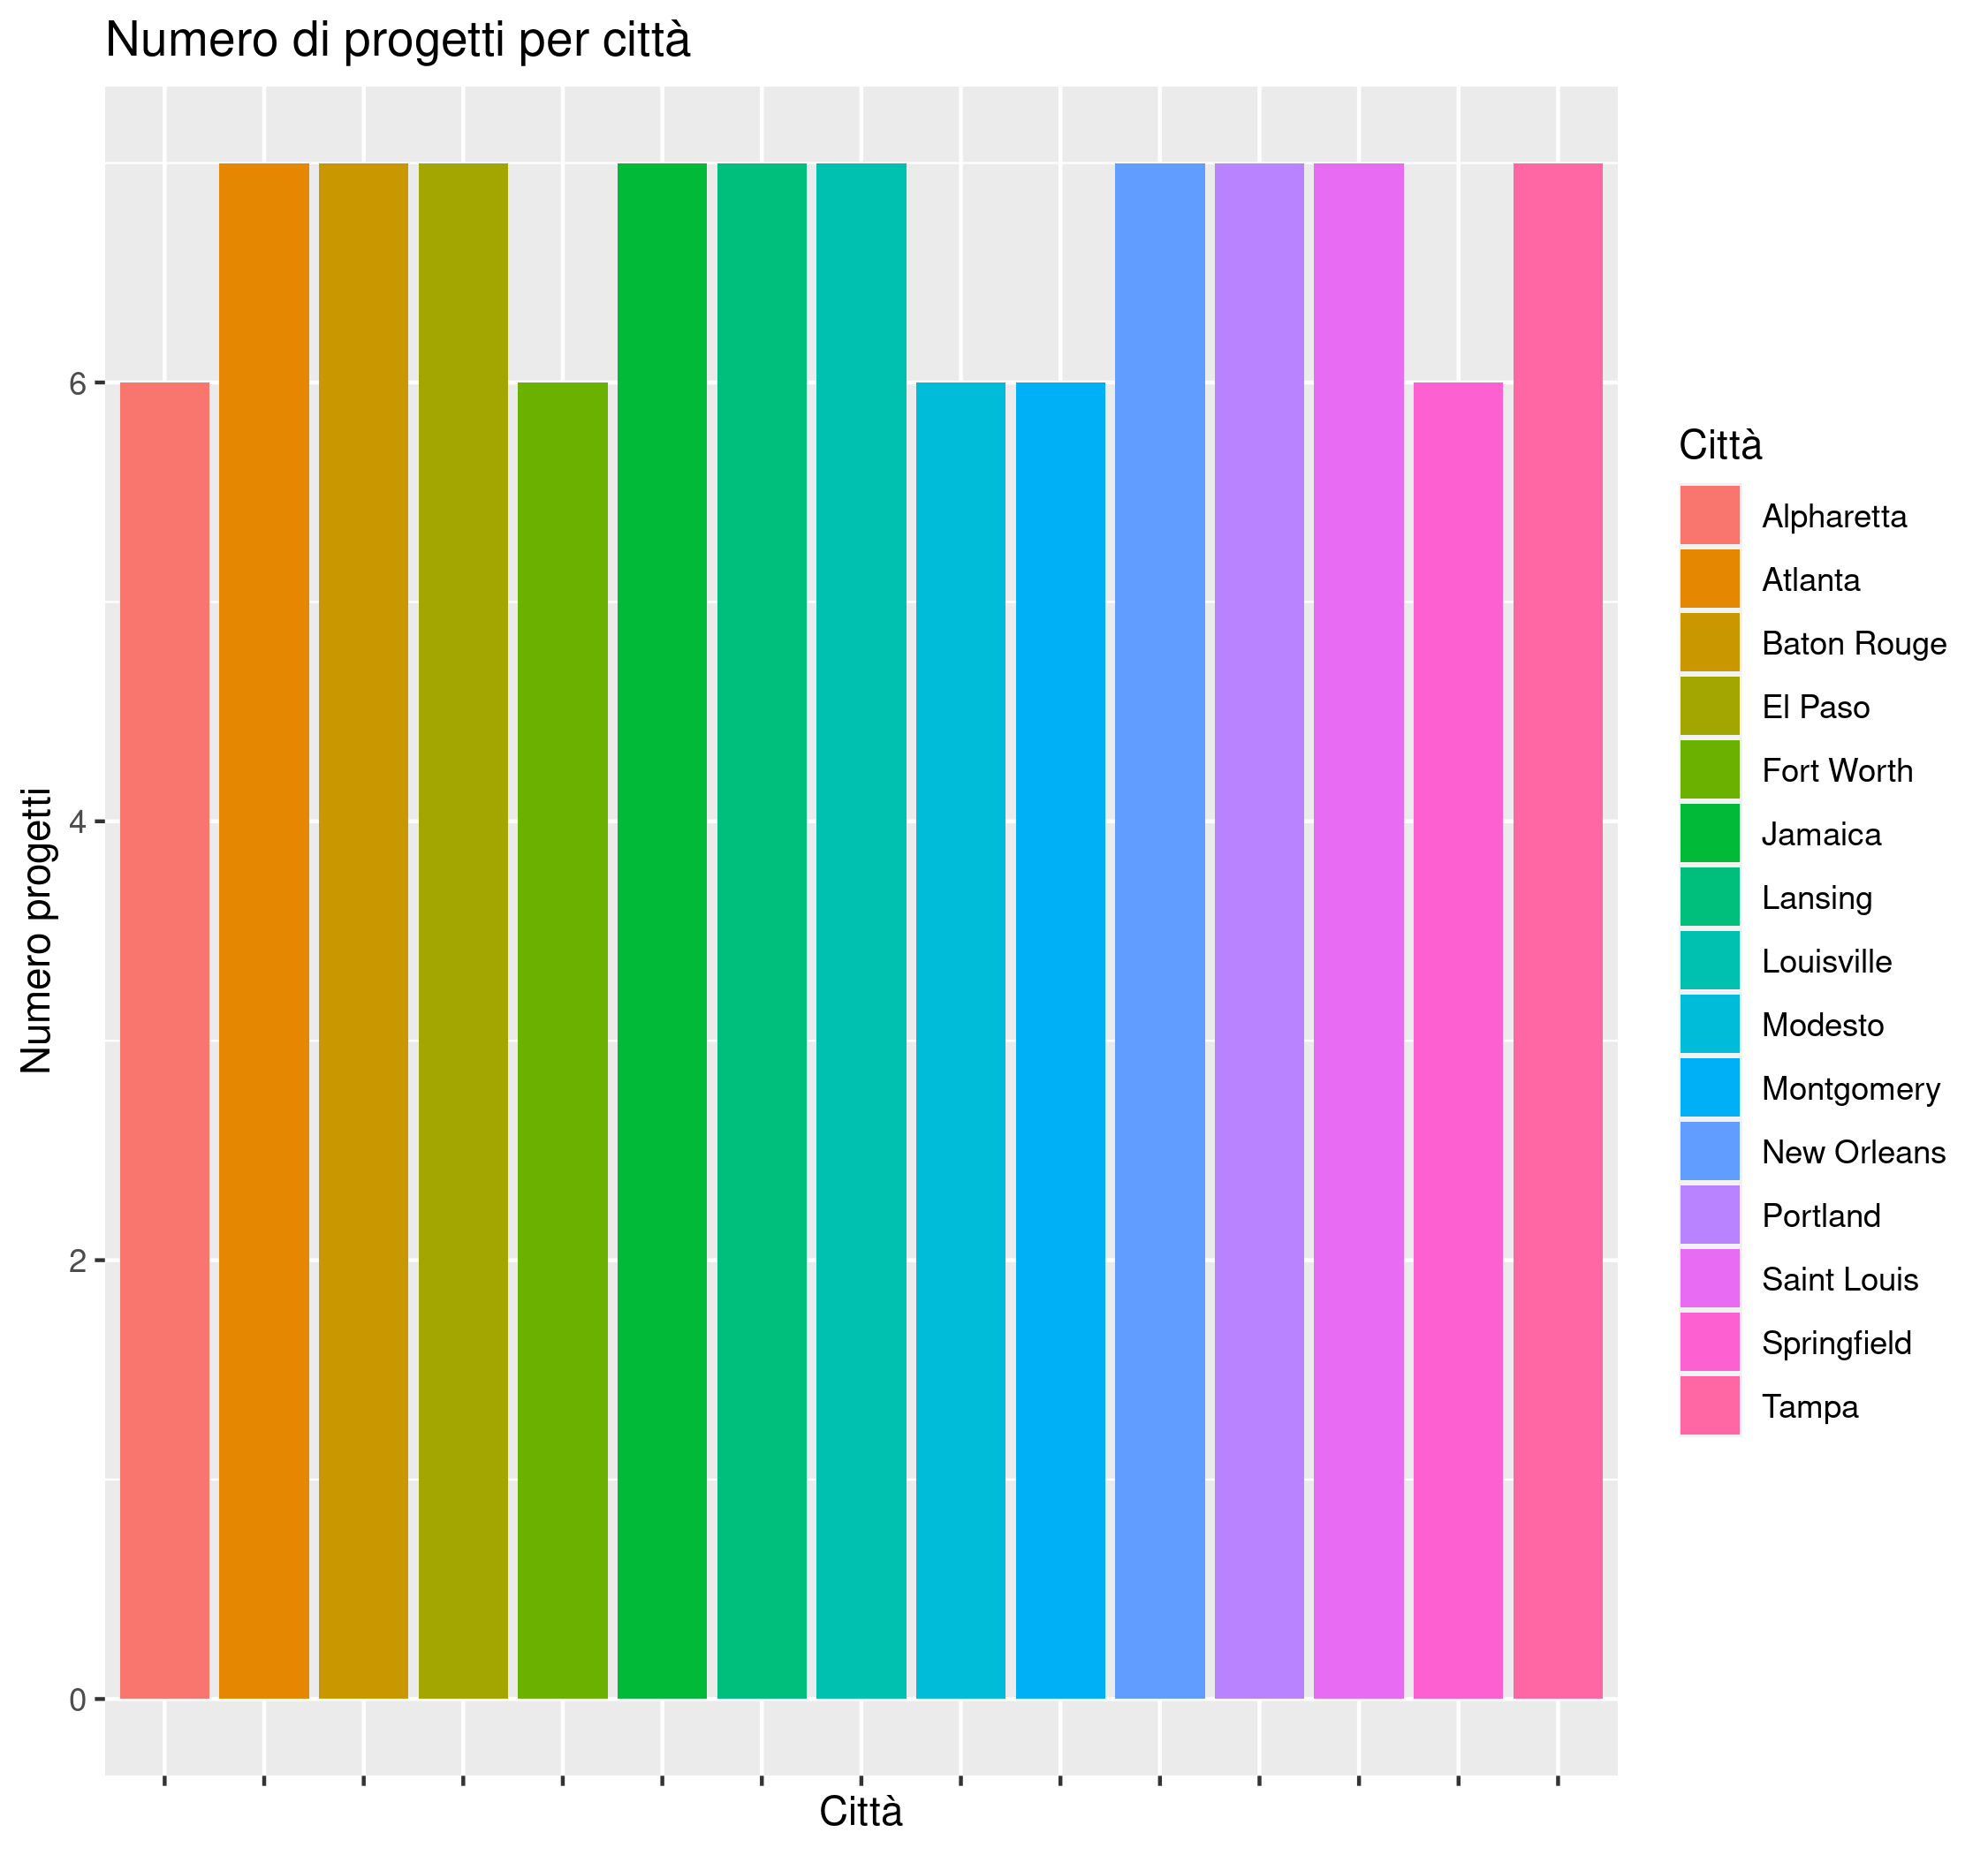
\includegraphics[width=\textwidth]{plot_numero_progetti_citta.png}
\end{center}

\newpage

\subsection{Distribuzione data di nascita per qualifica}
\begin{minted}{sql}
SELECT data_di_nascita, qualifica
FROM impiegato;
\end{minted}
\begin{center}
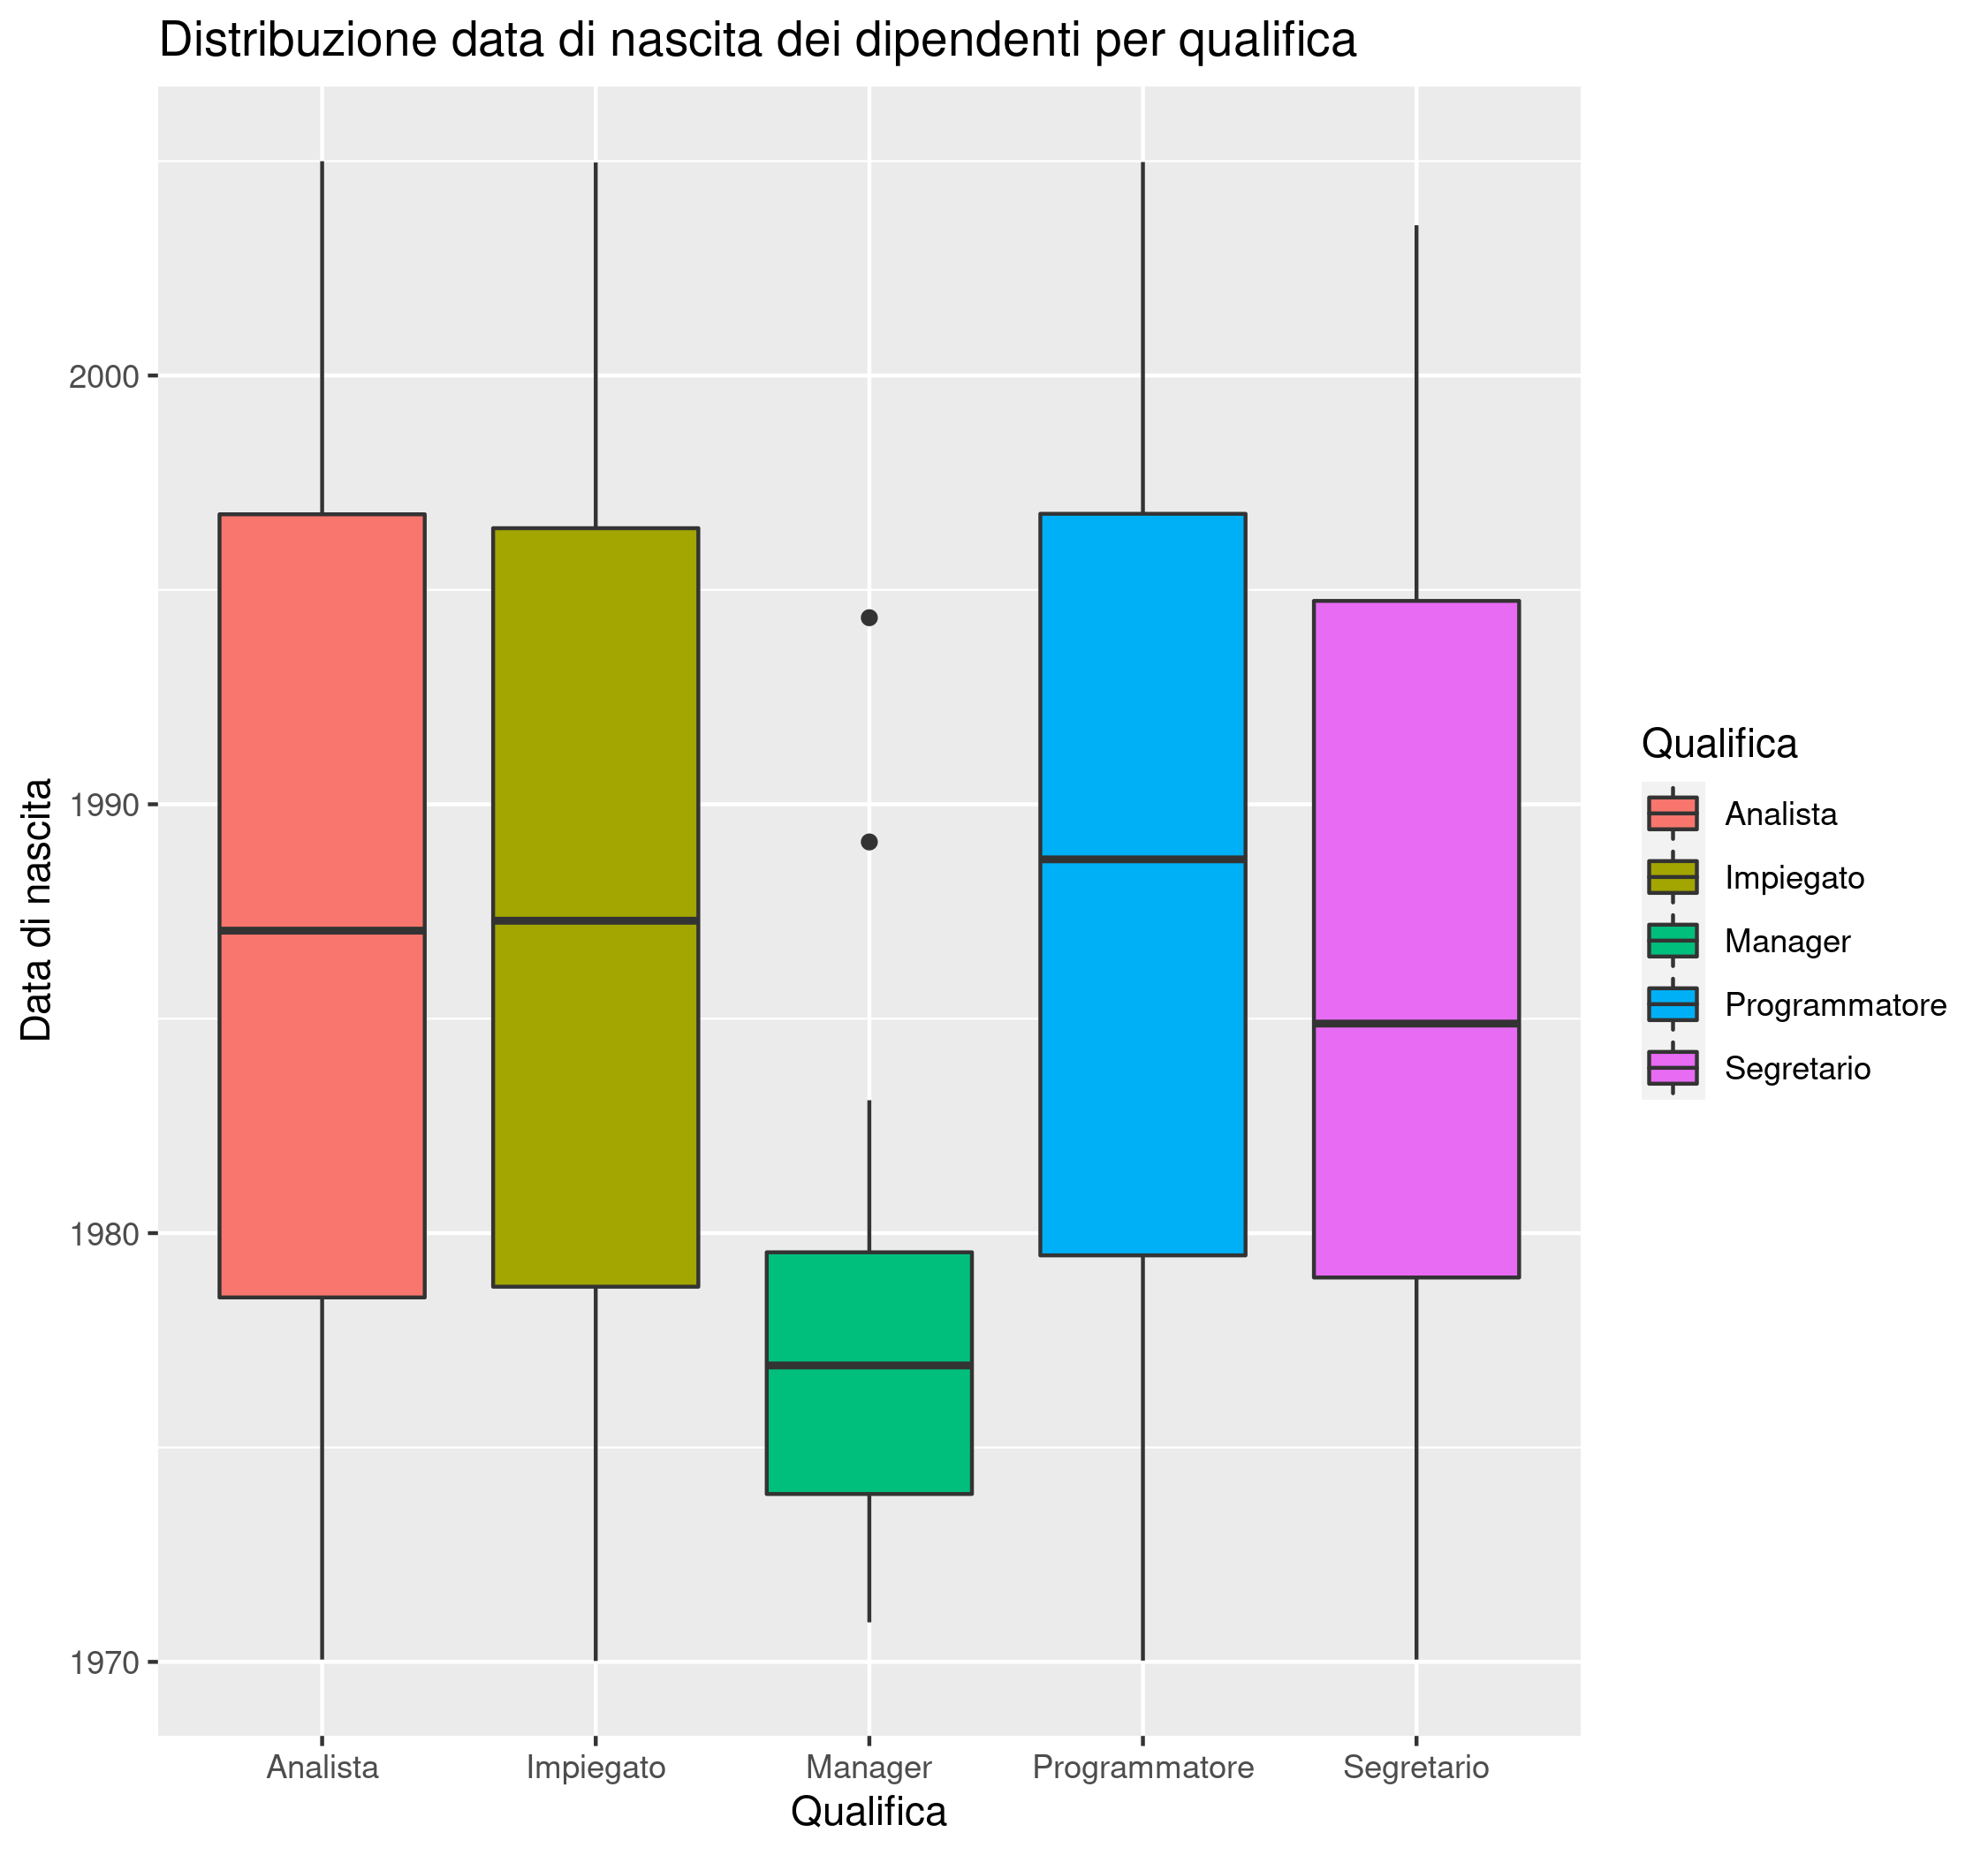
\includegraphics[width=\textwidth]{plot_dist_dNascita_qualifica.png}
\end{center}

\newpage

\subsection{Numero segretari per lingua}
\begin{minted}{sql}
SELECT lingua, count(*) 
FROM segretario 
GROUP BY lingua 
ORDER BY lingua;
\end{minted}
\begin{center}
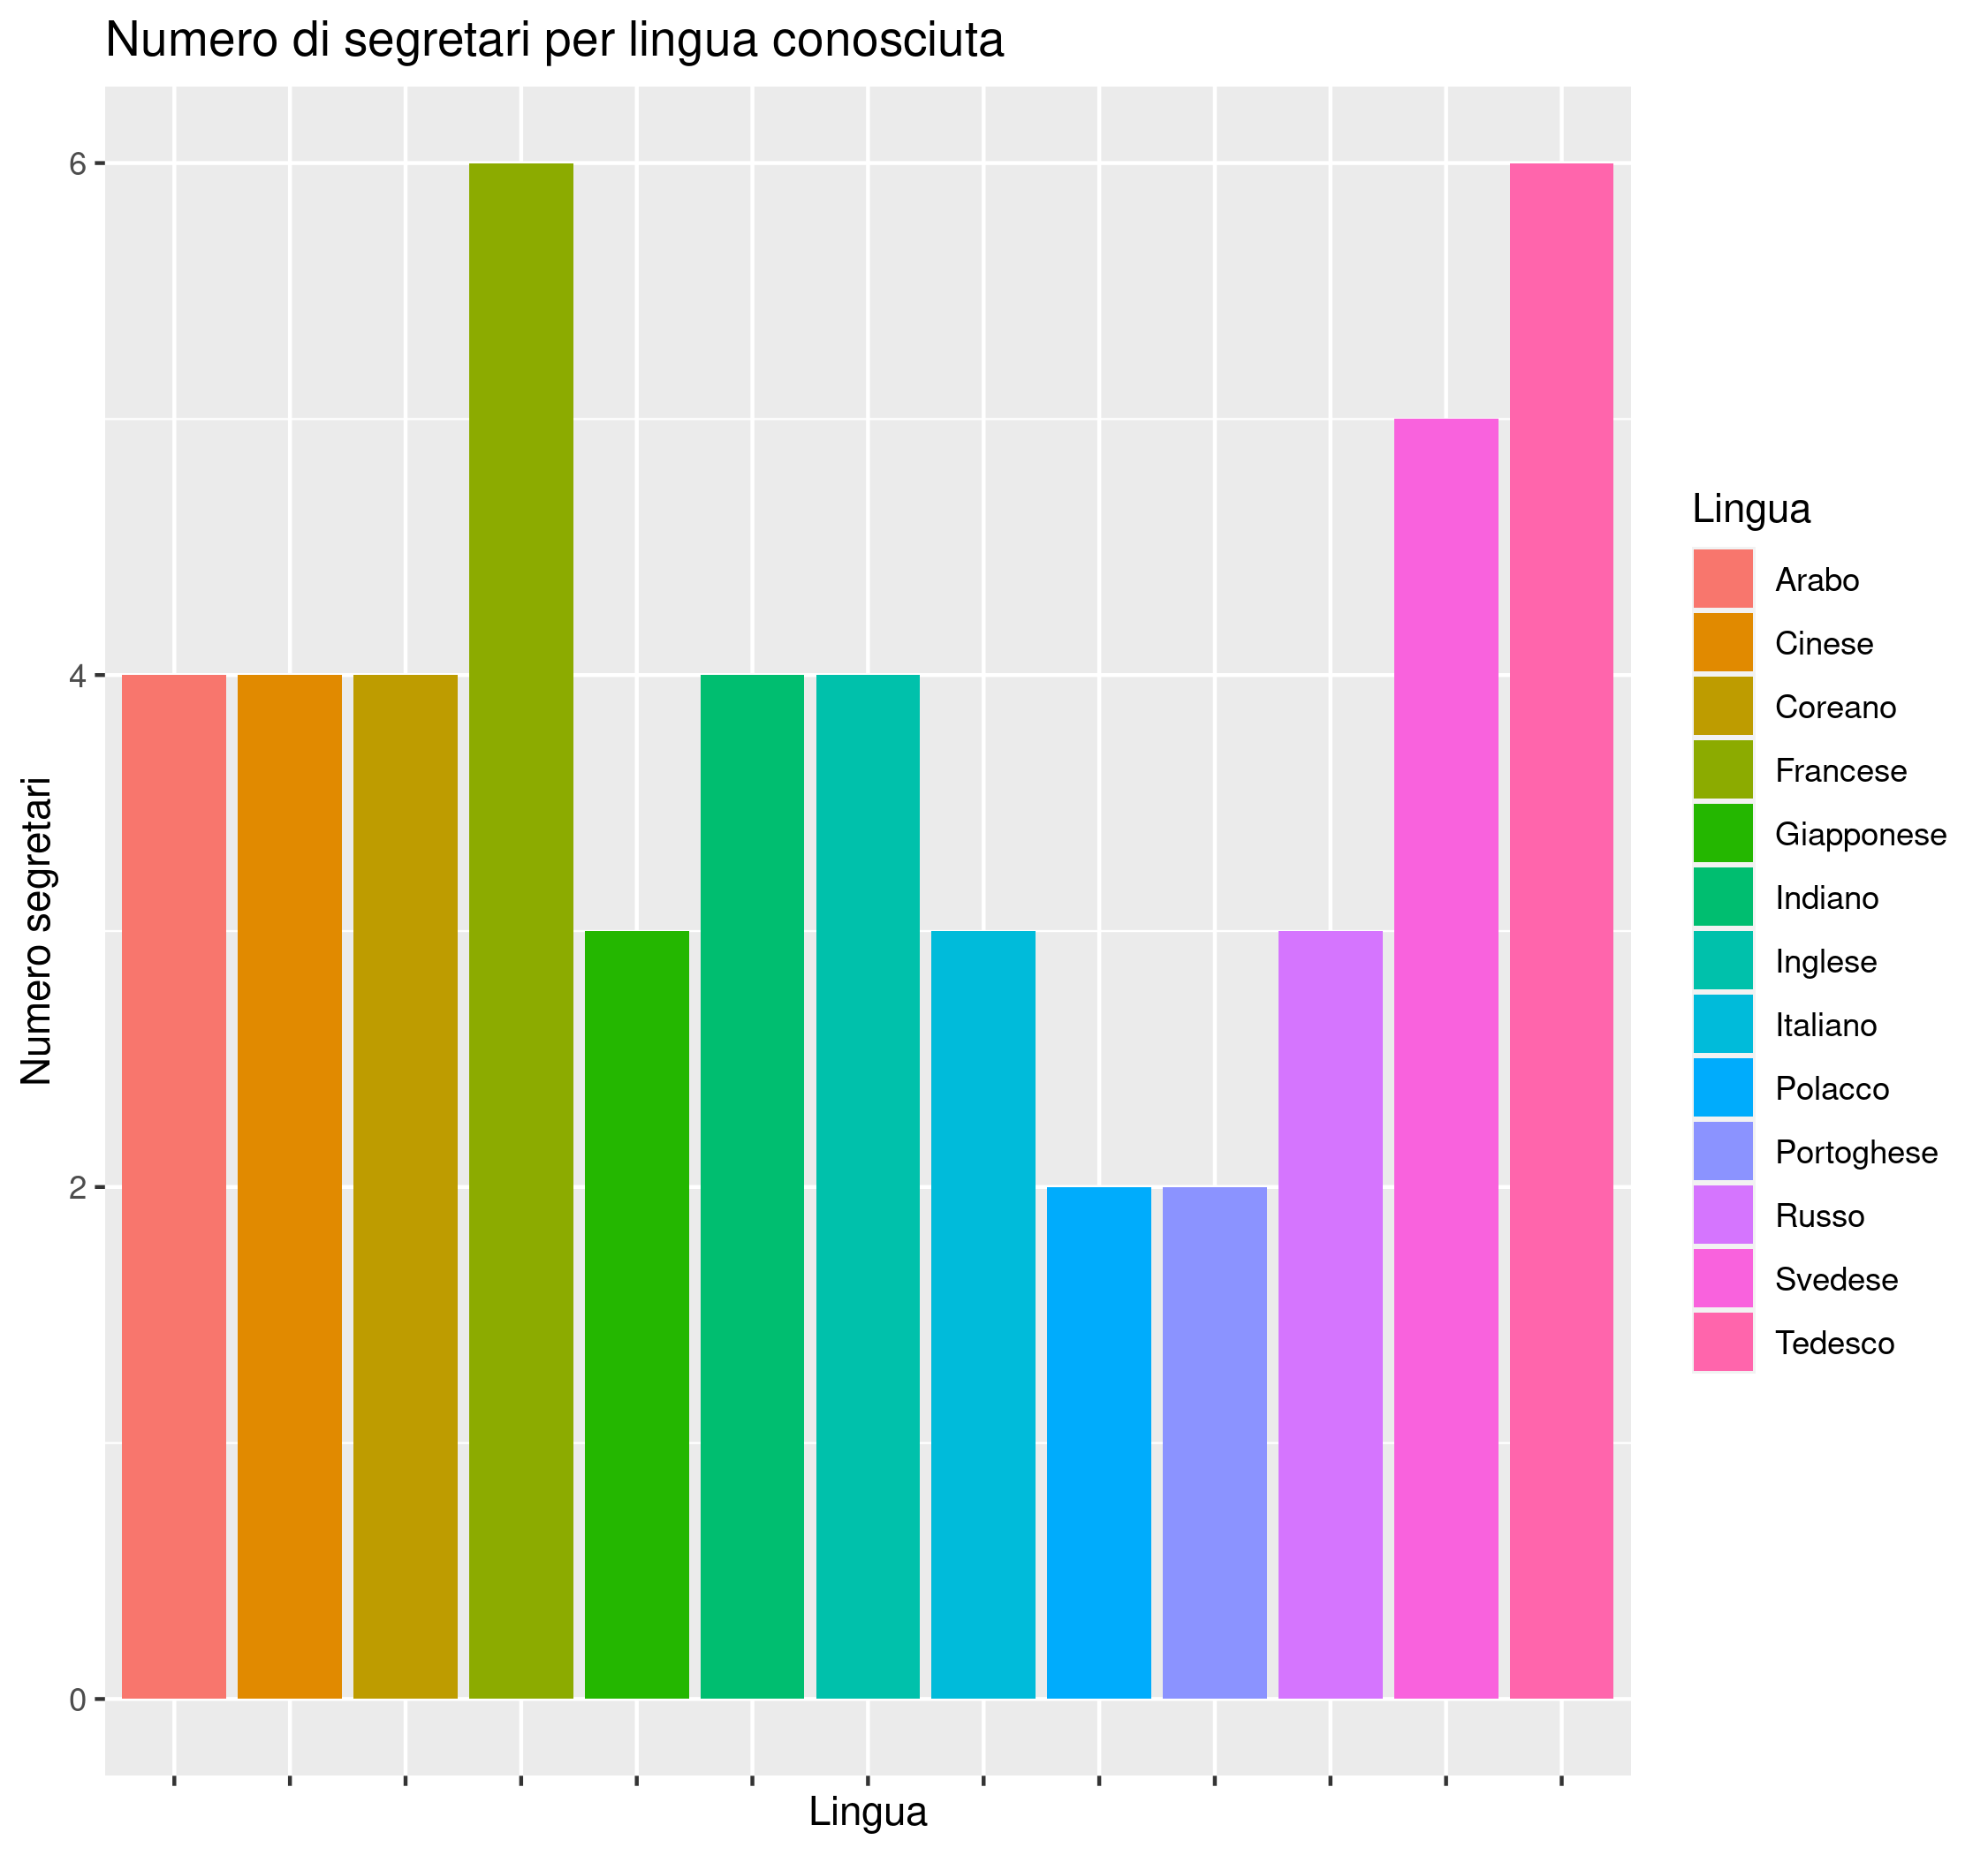
\includegraphics[width=\textwidth]{plot_numero_segretari_lingua.png}
\end{center}

\newpage

\subsection{Distribuzione budget per città}
\begin{minted}{sql}
SELECT budget, citta 
FROM progetto;
\end{minted}
\begin{center}
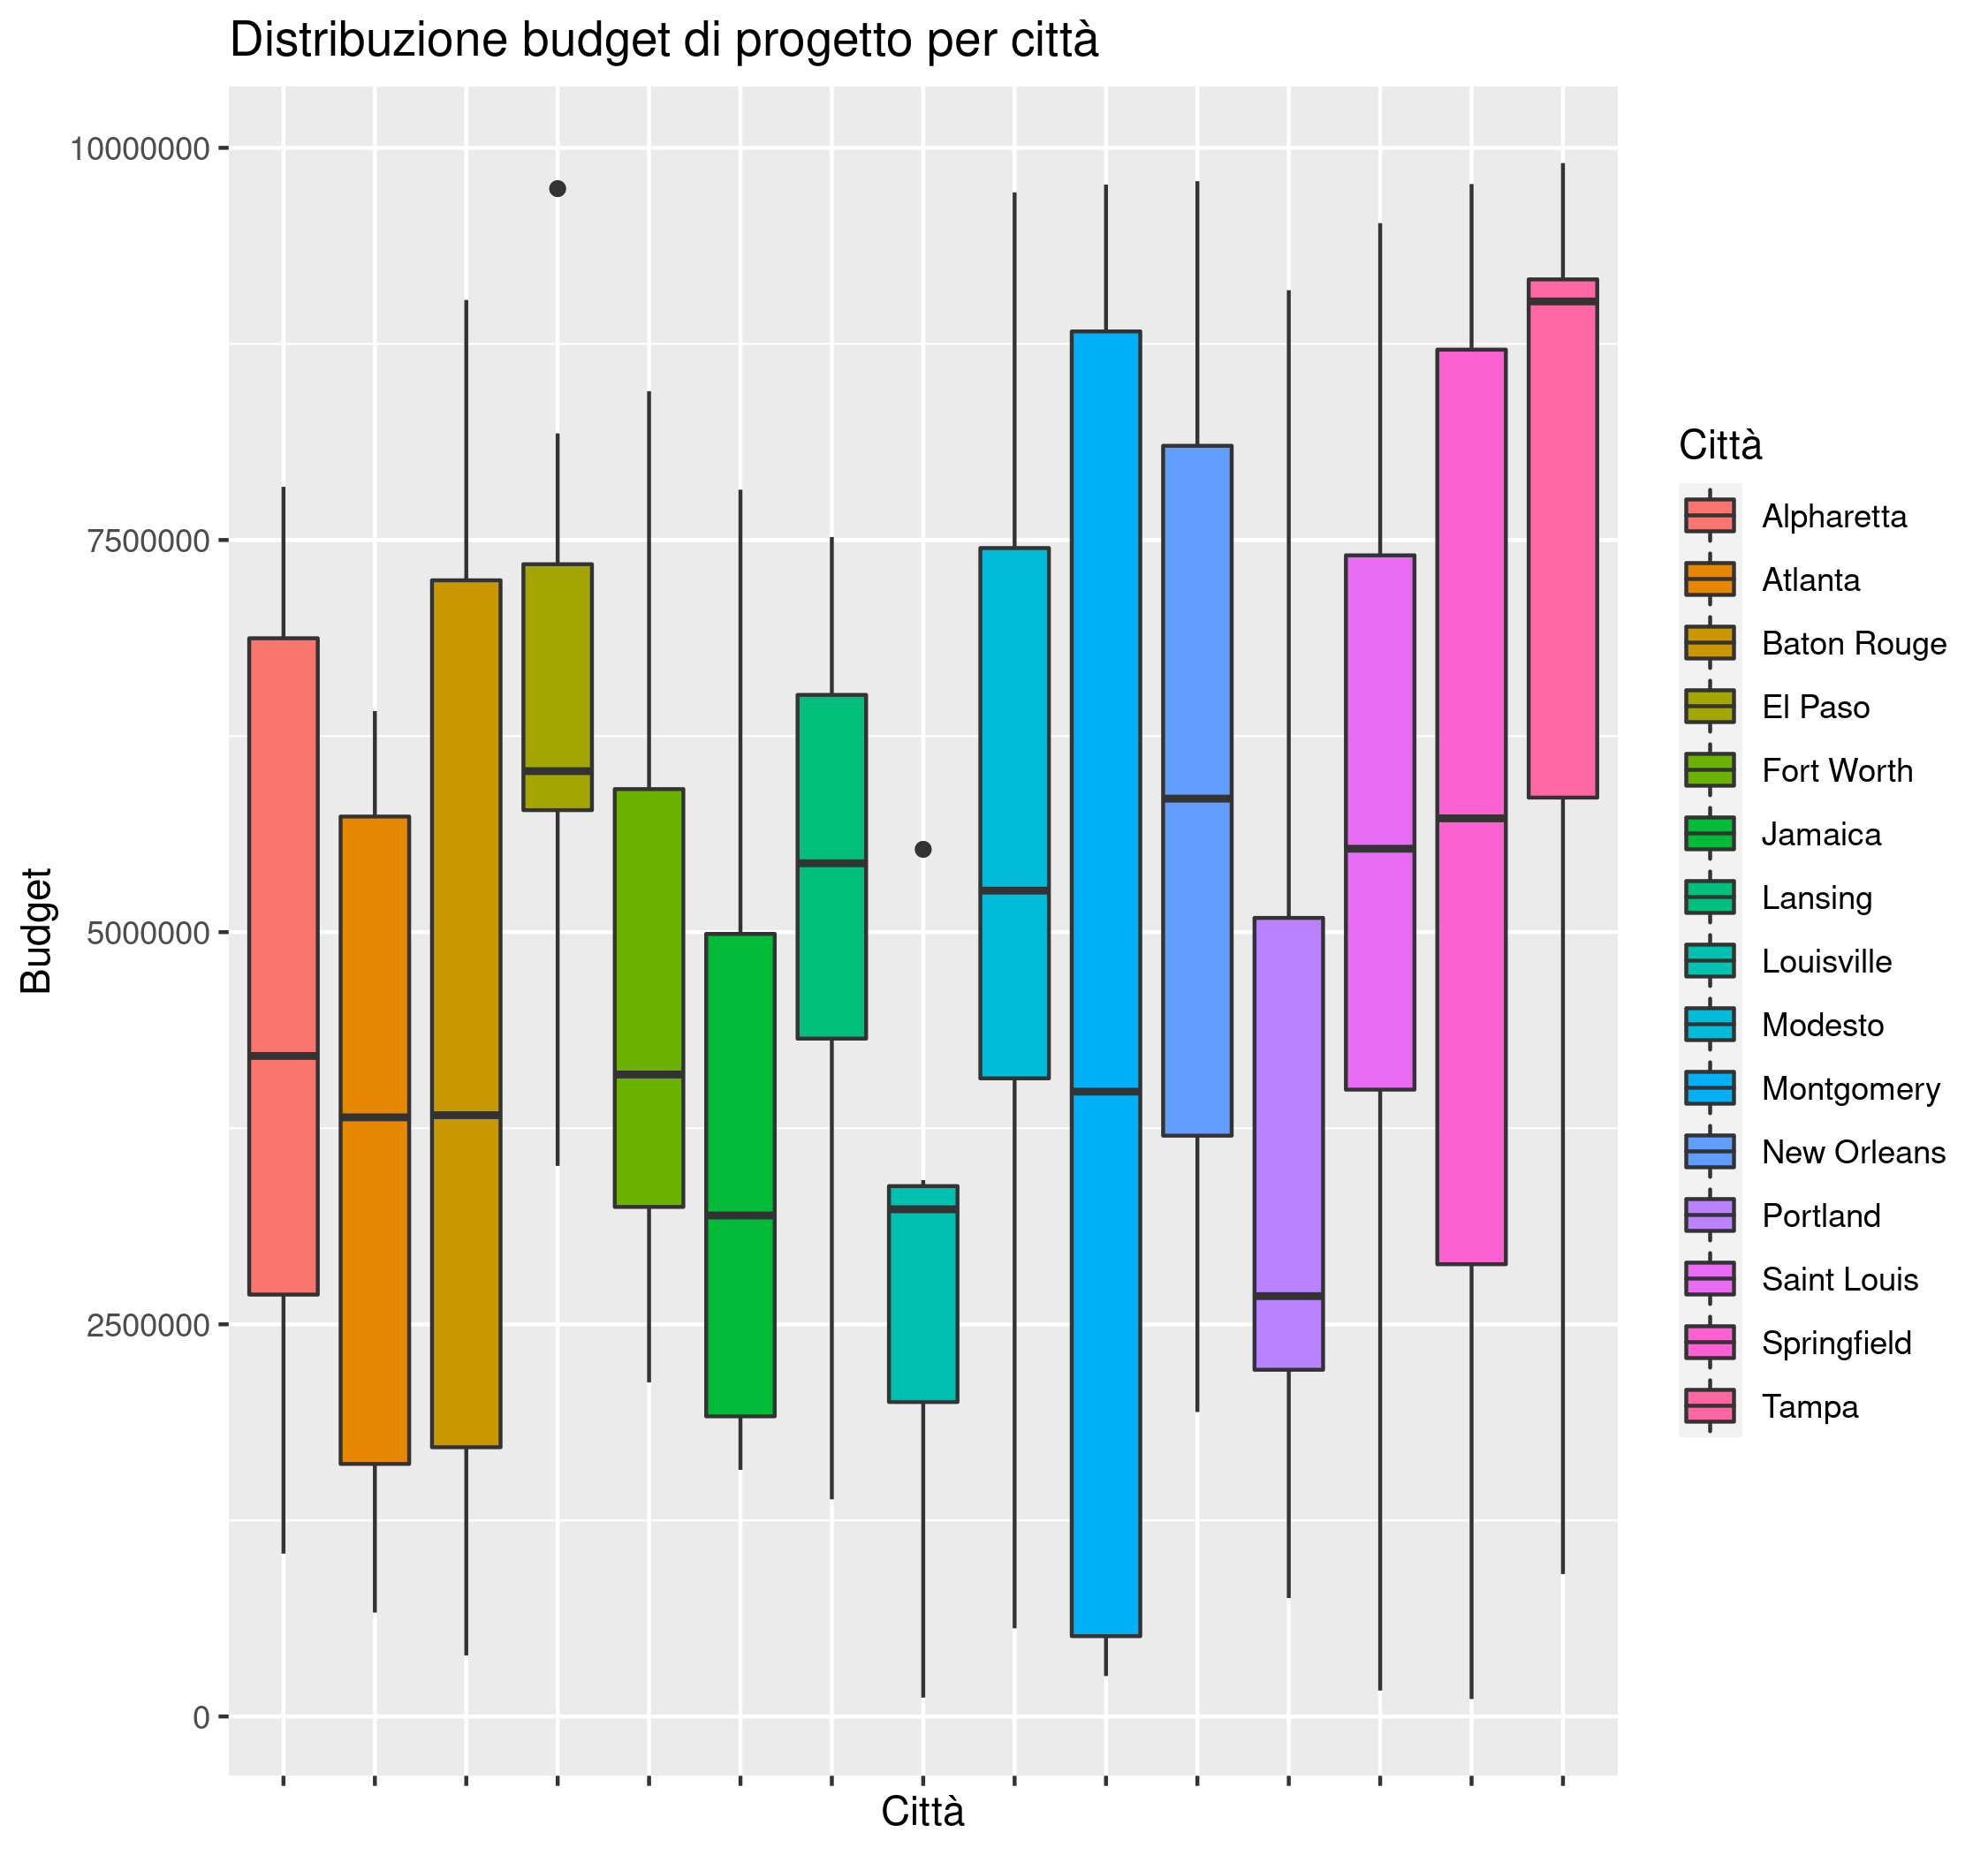
\includegraphics[width=\textwidth]{plot_dist_budget_progetto_citta.png}
\end{center}

\newpage

\subsection{Distribuzione partecipazioni a progetto con competenze}
\begin{minted}{sql}
SELECT descrizione, COUNT(*) FROM competenza, partecipa 
WHERE codice = partecipa.competenza 
GROUP BY codice 
ORDER BY descrizione;
\end{minted}
\begin{center}
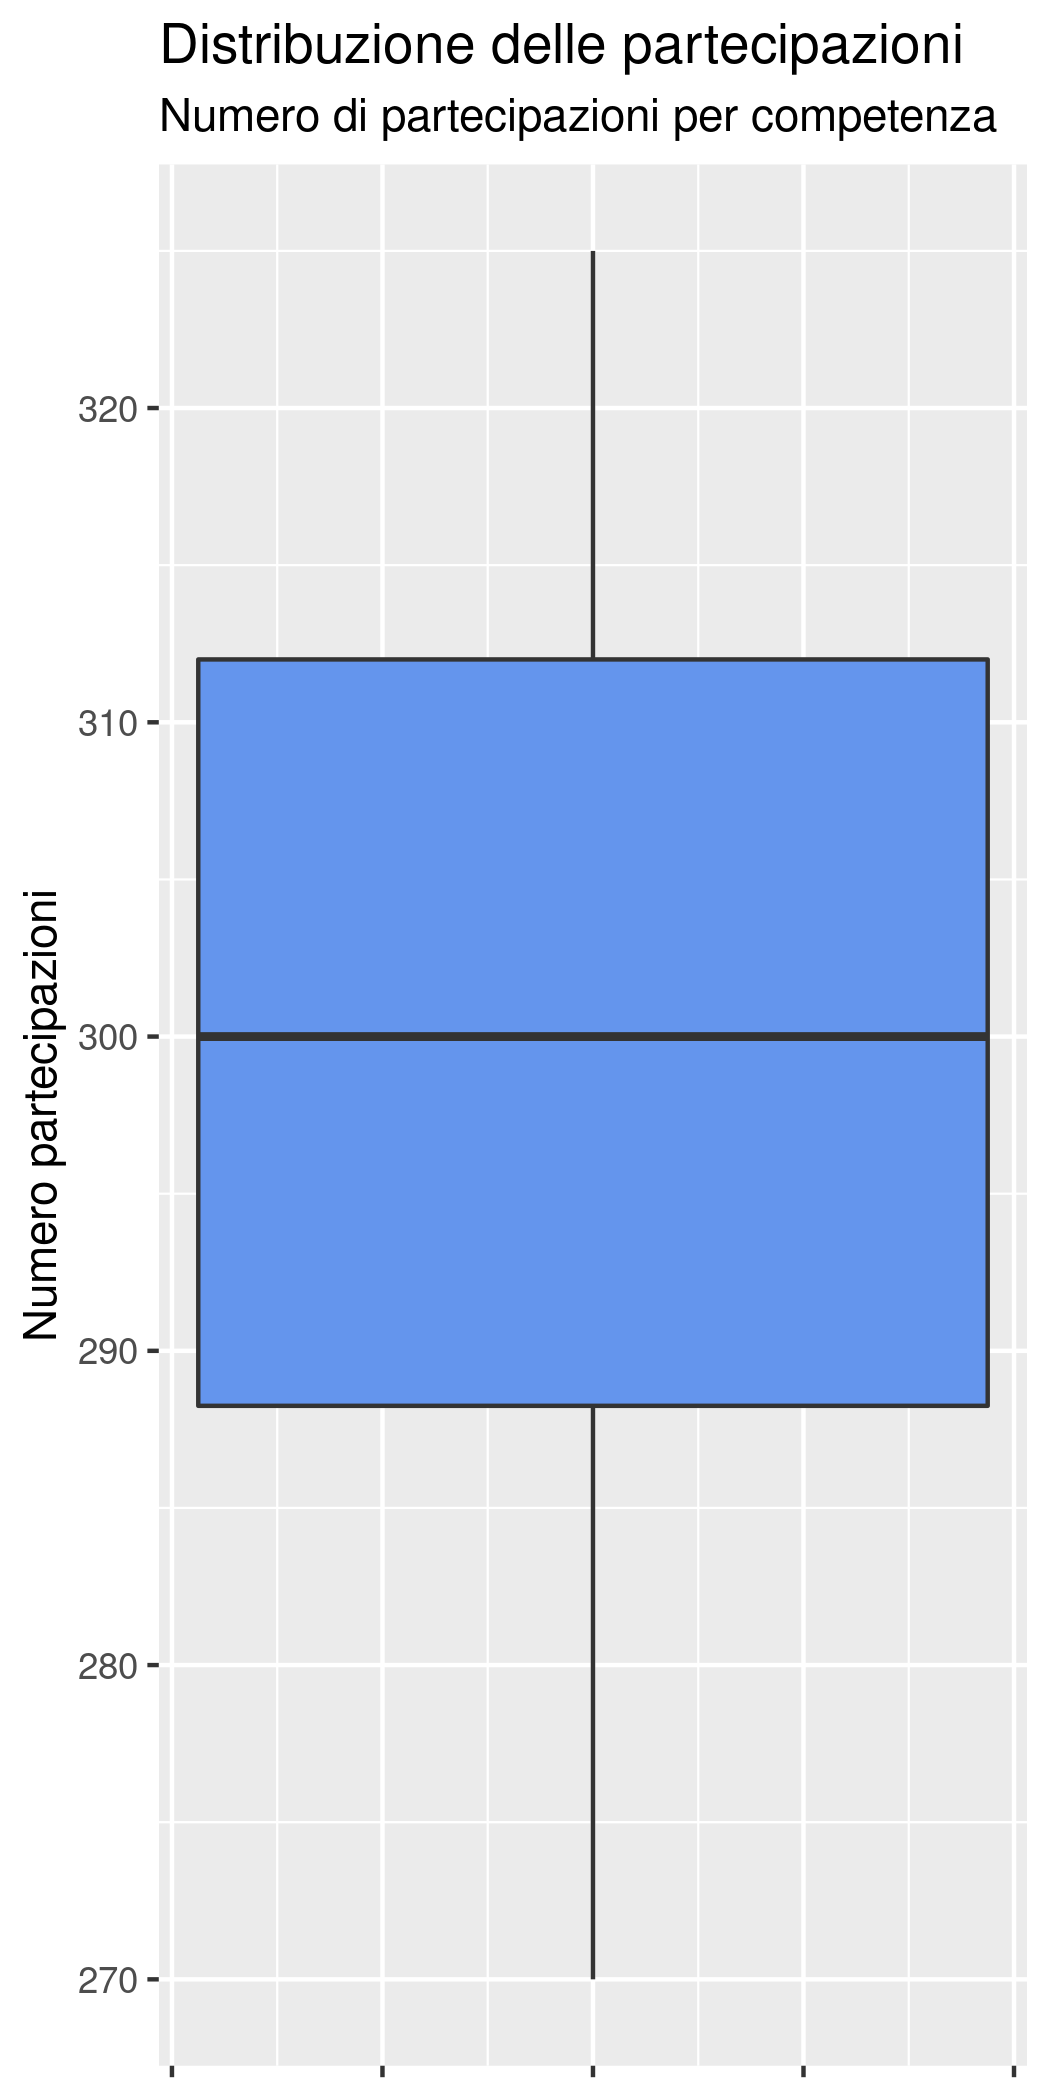
\includegraphics[width=.5\textwidth]{plot_dist_partecipazioni_comptenza.png}
\end{center}

\newpage

\subsection{Distribuzione impiegati per dipartimento}
\begin{minted}{sql}
SELECT dipartimento, COUNT(*) 
FROM impiegato, partecipa 
WHERE matricola = partecipa.impiegato 
GROUP BY dipartimento 
ORDER BY dipartimento
\end{minted}
\begin{center}
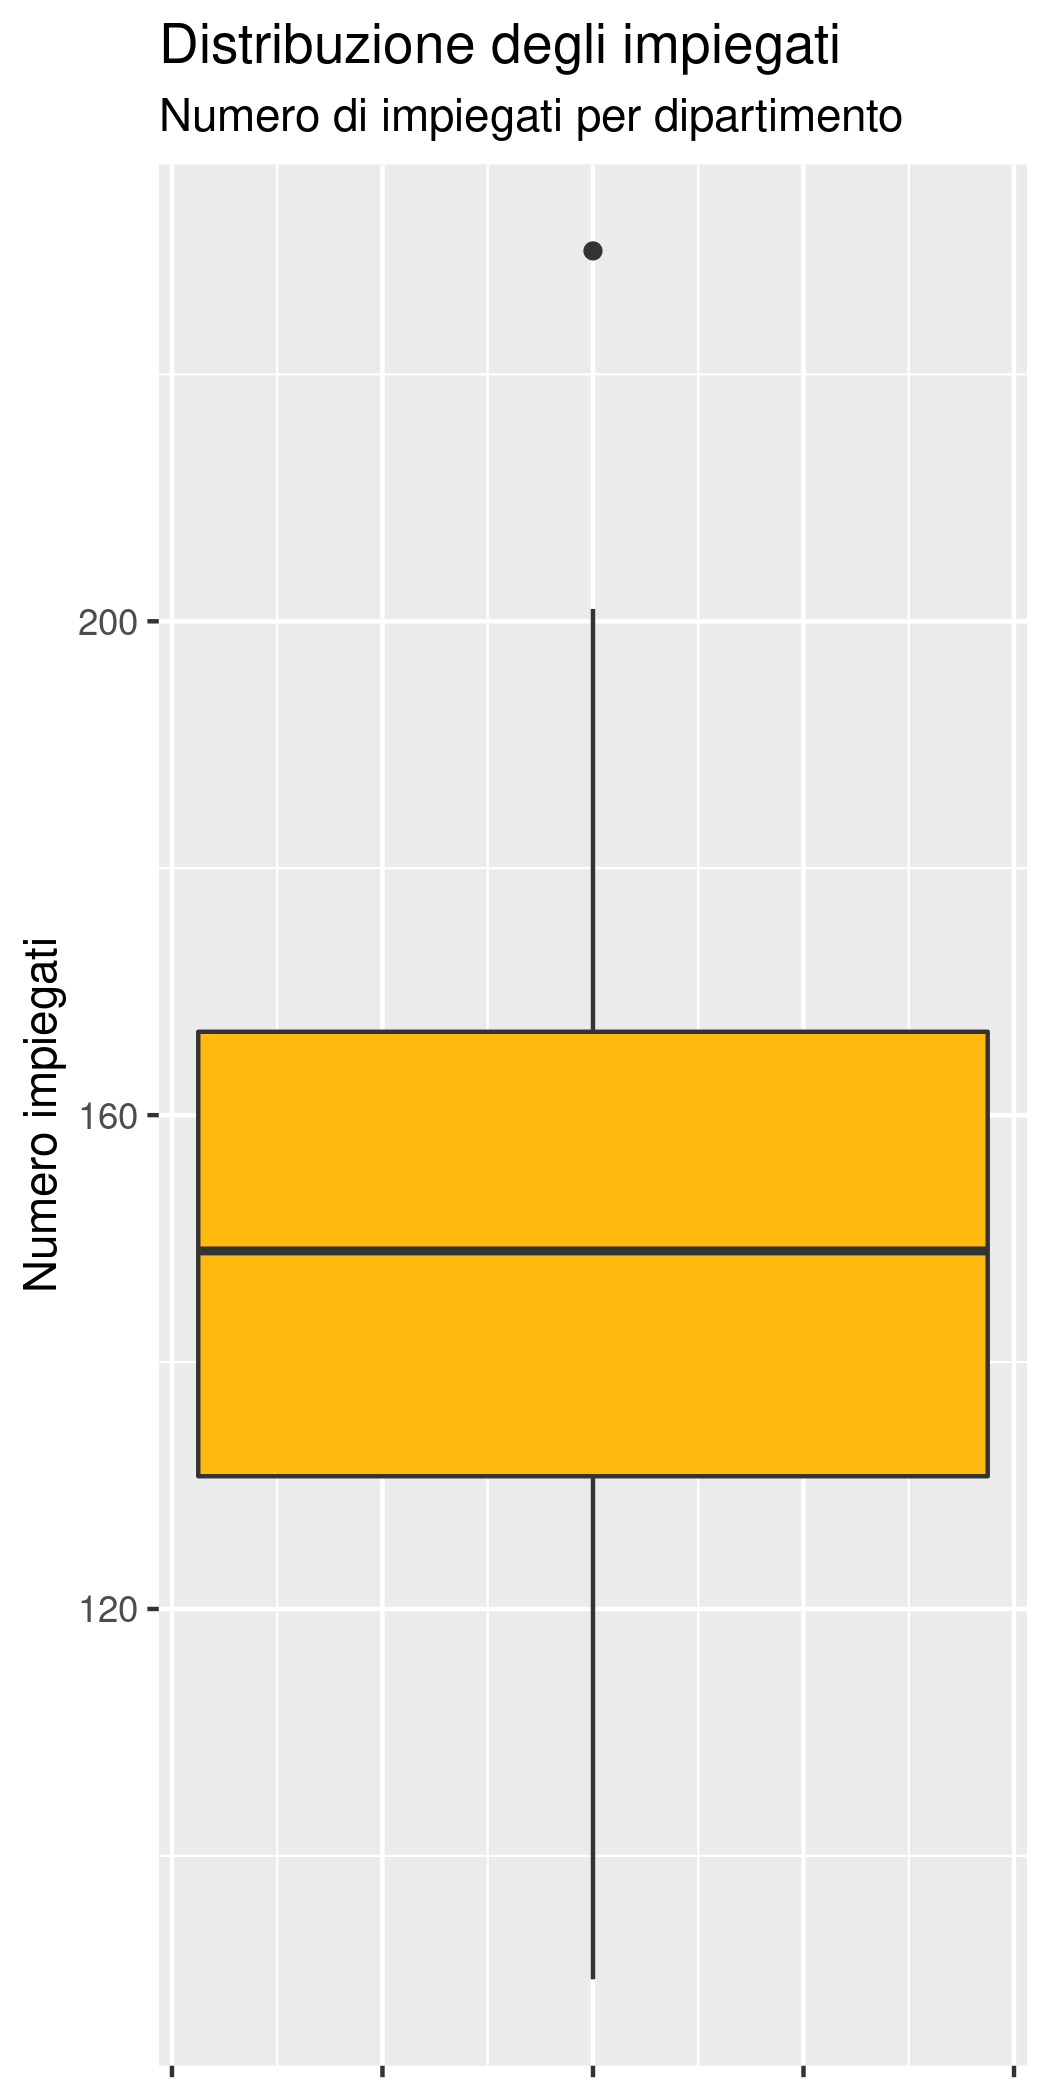
\includegraphics[width=.5\textwidth]{plot_dist_impiegati_dipartimento.png}
\end{center}

\newpage

\subsection{Percentuale impiegati laureati}
\begin{minted}{sql}
SELECT COUNT(*) 
FROM laureato 
UNION 
SELECT COUNT(*) 
FROM impiegato 
WHERE NOT EXISTS(
    SELECT * 
    FROM laureato 
    WHERE matricola = laureato.impiegato
    );
\end{minted}
\begin{center}
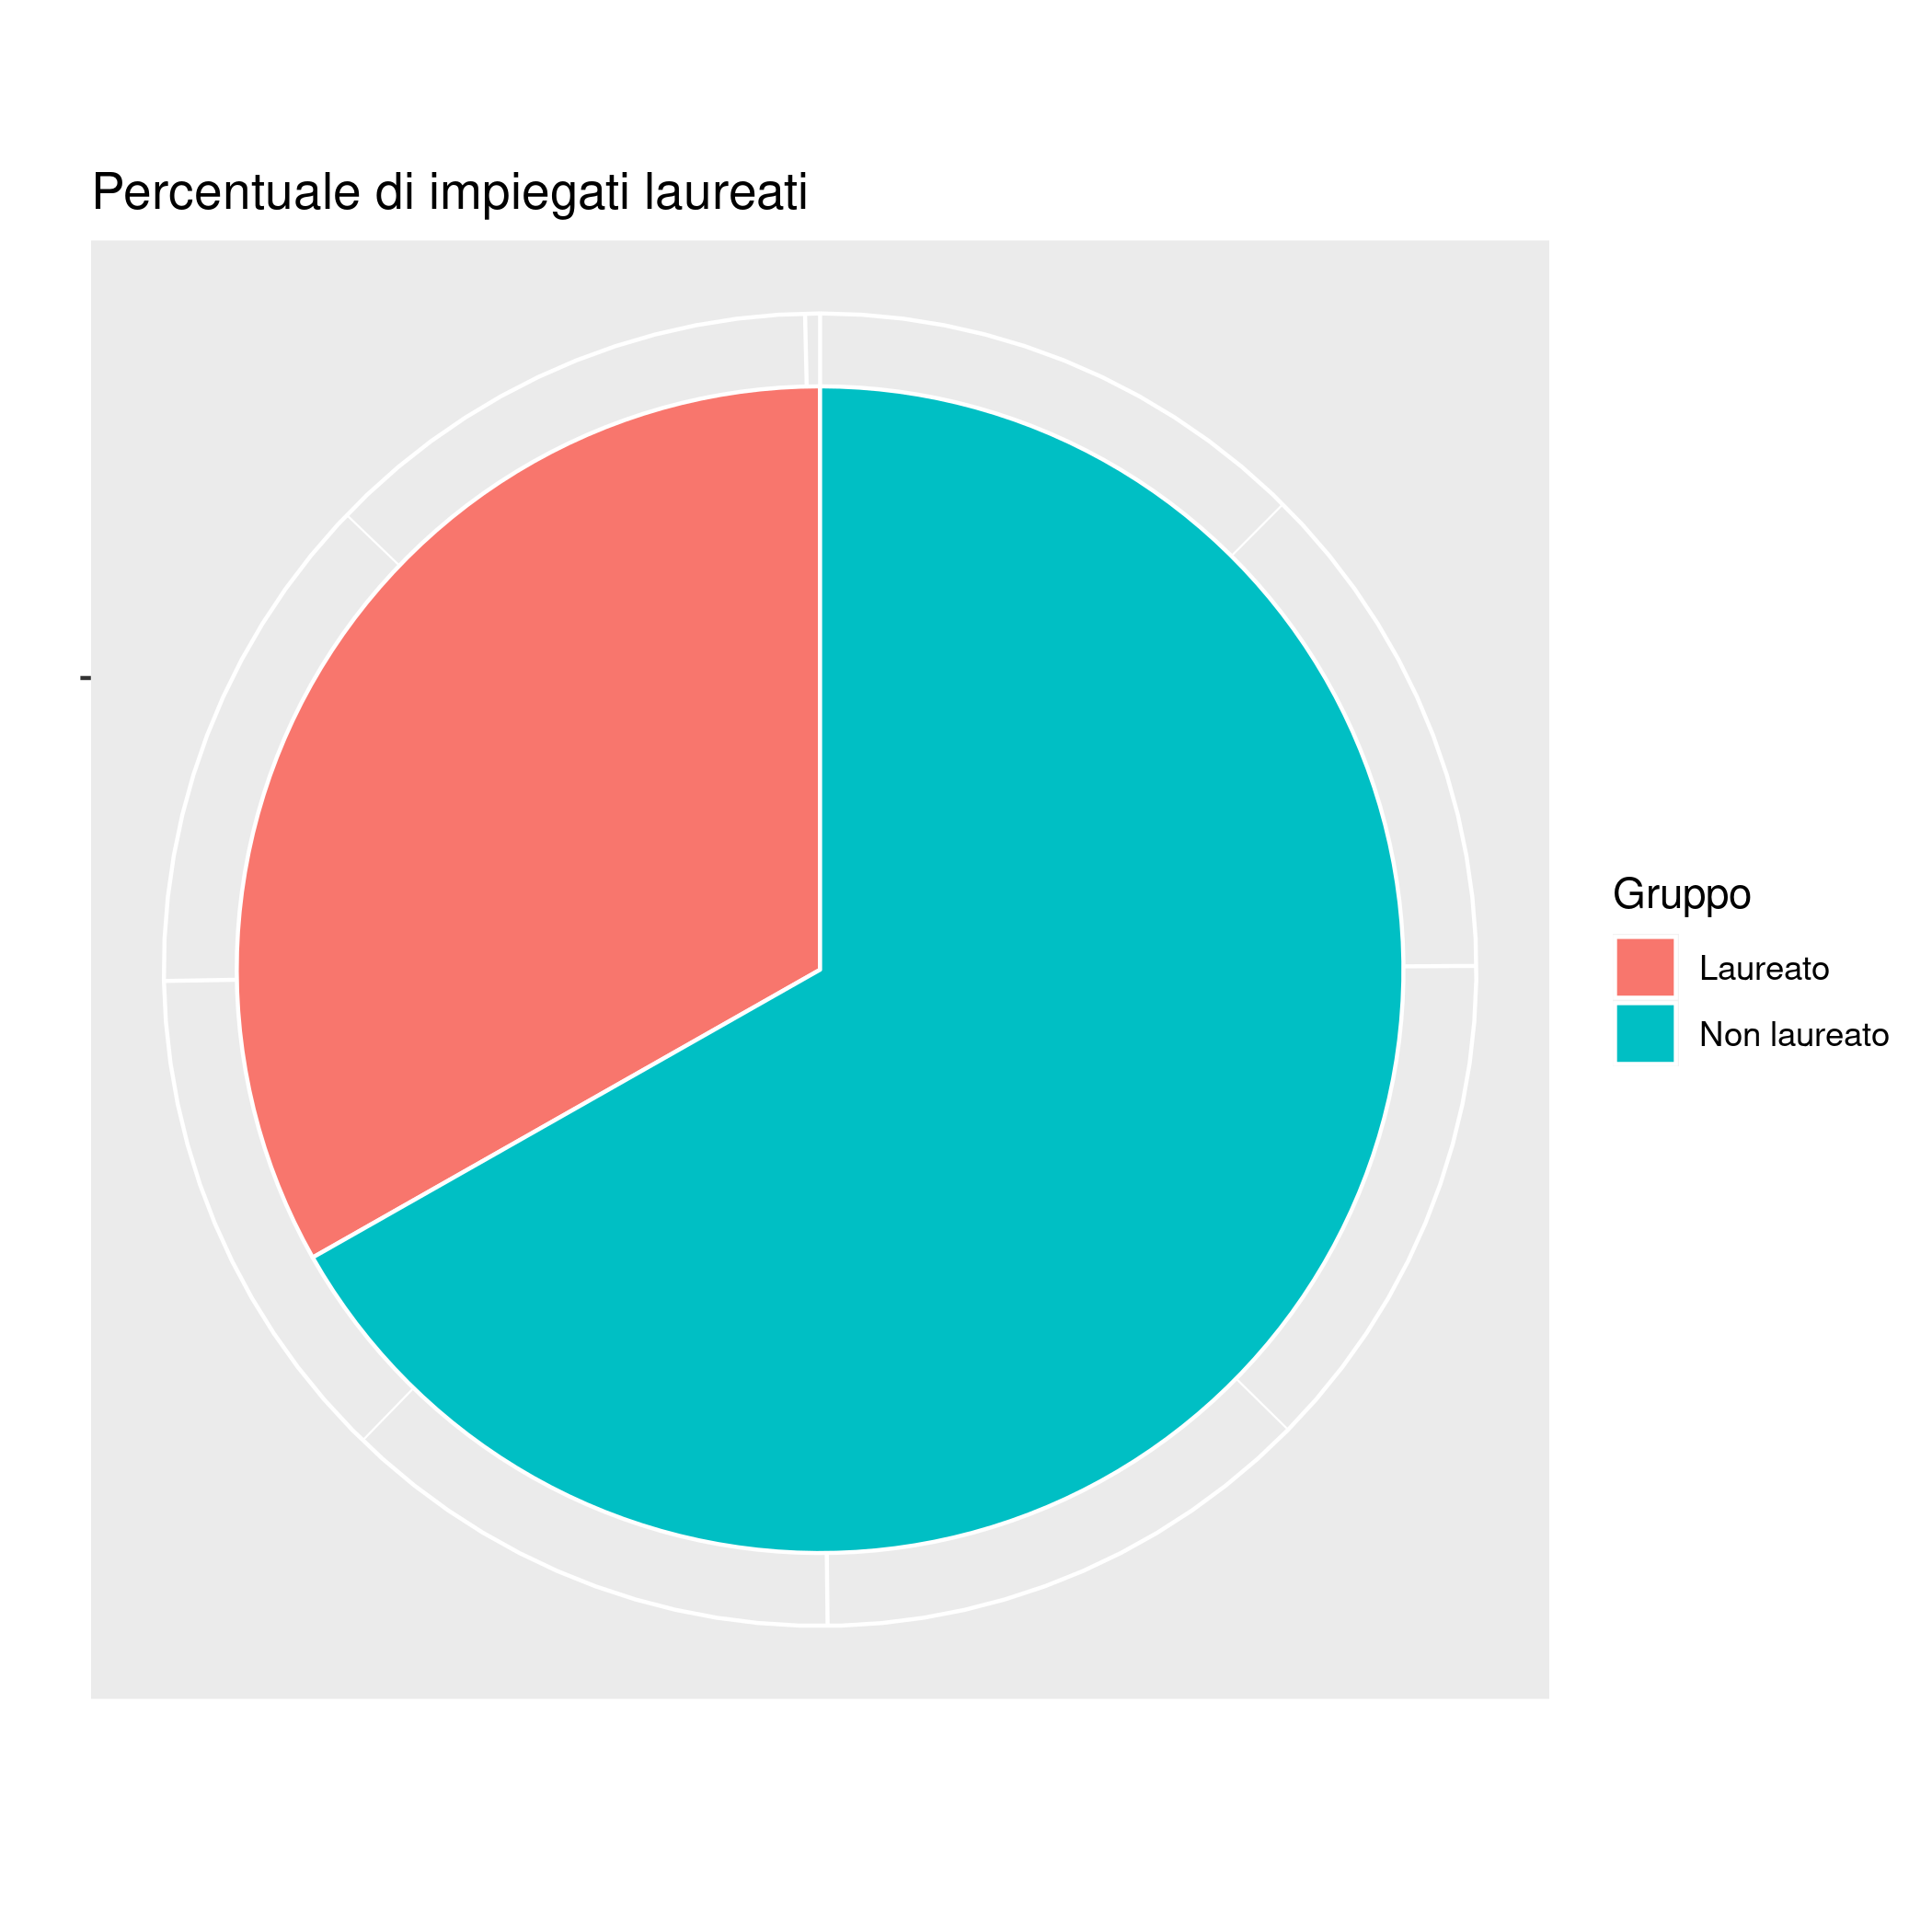
\includegraphics[width=\textwidth]{plot_perc_laureati.png}
\end{center}

\newpage

\subsection{Percentuale impiegati per qualifica}
\begin{minted}{sql}
SELECT qualifica, COUNT(*)/(SUM(COUNT(*)) OVER()) AS frequenza 
FROM impiegato 
GROUP BY qualifica;
\end{minted}
\begin{center}
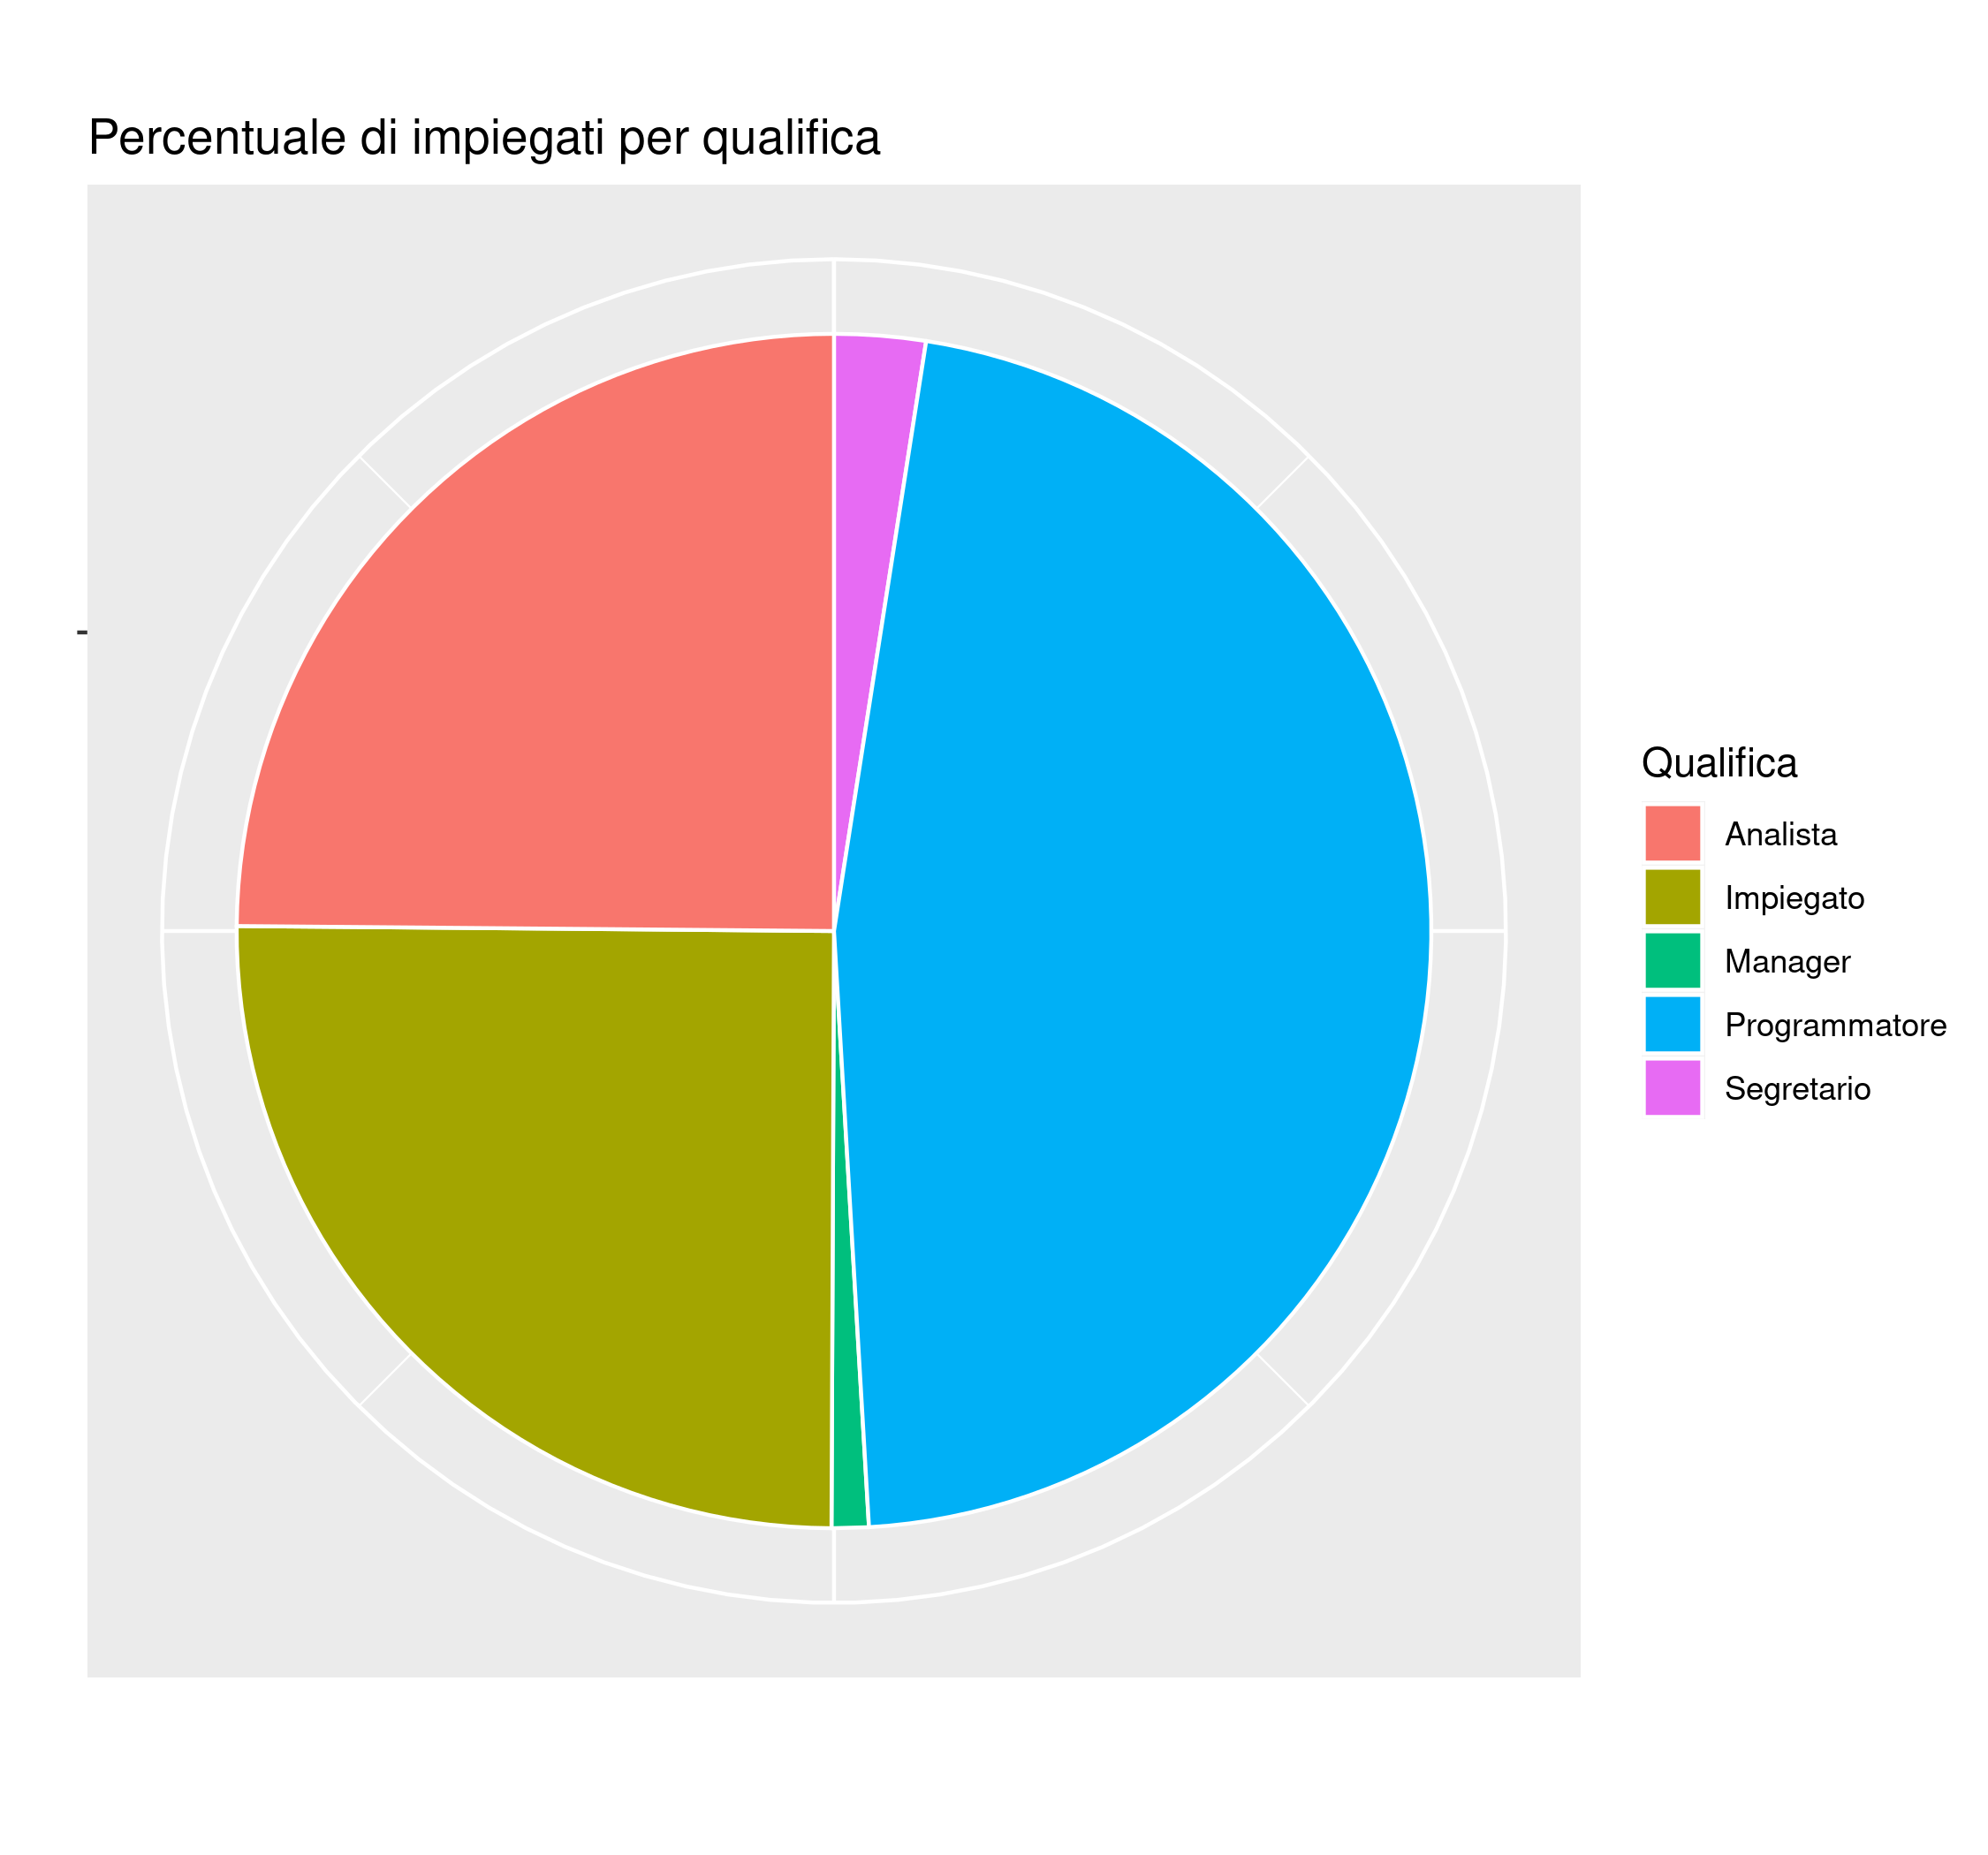
\includegraphics[width=\textwidth]{plot_perc_impiegati_qualifica.png}
\end{center}

\newpage

\section{Conclusioni}

\end{document}

